% Retoca las líneas marcadas con TODO según las necesidades

\documentclass[oneside,a4paper,12pt]{book} % TODO: cambia "oneside" por "twoside" a la hora de imprimirlo

\usepackage[spanish]{babel}
\usepackage[utf8]{inputenc}
\usepackage{geometry}
\usepackage{makeidx}
\usepackage{url}
\usepackage{graphicx}
\usepackage{color}
\usepackage{caption}
\usepackage{acronym}
\usepackage{hyphenat}
\usepackage{a4wide}
\usepackage[normalsize]{subfigure}
\usepackage{float}
\usepackage{titlesec}
\usepackage[export]{adjustbox}
\usepackage[Lenny]{fncychap}
\usepackage{listings} % para poder hacer uso de "listings" propios (p.ej. códigos)
\usepackage{eurosym} % para poder usar el símbolo del euro con \euro {xx}
\usepackage{hyperref} % TODO: añade la opción hidelinks para imprimirlo (los enlaces no aparecerán resaltados)

% Para que no parta las palabras
\pretolerance=10000

\newcommand{\bigrule}{\titlerule[0.5mm]} \titleformat{\chapter}[display] % cambiamos el formato de los capítulos
{\bfseries\Huge} % por defecto se usaron caracteres de tamaño huge en negrita
{% contenido de la etiqueta 
\titlerule % línea horizontal 
\filright % texto alineado a la derecha 
\Large\chaptertitlename\ % capítulo e índice en tamaño large
\Large % en lugar de 
\Huge \Large\thechapter} 
{0mm} % espacio mínimo entre etiqueta y cuerpo
{\filright} % texto del cuerpo alineado a la derecha
[\vspace{0.5mm} \bigrule] % después del cuerpo, dejar espacio vertical y trazar línea horizontal gruesa
\geometry{a4paper, left=3.5cm, right=2cm, top=3cm, bottom=2cm, headsep=1.5cm}

% Estilos para ilustrar códigos:
\definecolor{code_green}{rgb}{0,0.6,0}
\definecolor{code_gray}{rgb}{0.5,0.5,0.5}
\definecolor{code_mauve}{rgb}{0.58,0,0.82}

\lstset{frame=tb,
  language=C,
  aboveskip=3mm,
  belowskip=3mm,
  showstringspaces=false,
  columns=flexible,
  basicstyle={\small\ttfamily},
  numbers=none,
  numberstyle=\tiny\color{code_gray},
  keywordstyle=\color{blue},
  commentstyle=\color{code_green},
  stringstyle=\color{code_mauve},
  breaklines=true,
  breakatwhitespace=true,
  tabsize=3
}

\lstset{frame=tb,
  language=C++,
  aboveskip=3mm,
  belowskip=3mm,
  showstringspaces=false,
  columns=flexible,
  basicstyle={\small\ttfamily},
  numbers=none,
  numberstyle=\tiny\color{code_gray},
  keywordstyle=\color{blue},
  commentstyle=\color{code_green},
  stringstyle=\color{code_mauve},
  breaklines=true,
  breakatwhitespace=true,
  tabsize=3
}

\lstset{frame=tb,
  language=Python,
  aboveskip=3mm,
  belowskip=3mm,
  showstringspaces=false,
  columns=flexible,
  basicstyle={\small\ttfamily},
  numbers=none,
  numberstyle=\tiny\color{code_gray},
  keywordstyle=\color{blue},
  commentstyle=\color{code_green},
  stringstyle=\color{code_mauve},
  breaklines=true,
  breakatwhitespace=true,
  tabsize=3
}

% Definición de mis propios tipos: Códigos, Ecuaciones y Tablas
\DeclareCaptionType{code}[Código][Listado de códigos]
\DeclareCaptionType{myequation}[Ecuación][Listado de ecuaciones]

% TODO: especifica las reglas de separación que consideres. Algunos ejemplos:
\hyphenation{fuer-tes}
\hyphenation{mul-ti-ca-pa}
\hyphenation{res-pues-ta}
\hyphenation{di-fe-ren-tes}
\hyphenation{de-sa-rro-lla-dos}
\hyphenation{re-pre-sen-tan-do}

 % archivo de configuraci�n de estilo

\makeindex

\usepackage{array}
\usepackage{multirow}
\usepackage{caption} 
\usepackage{makecell}
\usepackage{amsmath}

\newcolumntype{P}[1]{>{\centering\arraybackslash}p{#1}}

\begin{document}
\baselineskip 1.35\baselineskip

\frontmatter

\thispagestyle{empty}
\vspace{2cm}

\begin{figure}[htb]
  \centerline{\resizebox{.45\textwidth}{!}{
\includegraphics{figs/logo_urjc}}}
\end{figure}

\begin{center}
  \vspace{5mm}
    {\Large {ESCUELA DE INGENIERÍA DE FUENLABRADA}}
  \vspace{1cm}
  
  {\Large {GRADO EN INGENIERÍA DE ROBÓTICA SOFTWARE}}
  \vspace{20mm}

   {\Large {\textbf{TRABAJO FIN DE GRADO}}}


   \vspace{2cm}

  {\large \textbf{Automatización de línea de producción robotizada  \\
              para simulación didáctica }}

  \vspace{2cm}
  
  {\bf Autor/a}: Álvaro Alonso Alosete
  
  {\bf Tutor}: Julio S. Lora Millán 

\vspace{3cm}

  Curso académico 2024 / 2025

 
\end{center}

\clearpage
\thispagestyle{empty}


% Este diseño se corresponde con la licencia CC-BY-NC-SA.
% Por supuesto, puedes poner la licencia que mejor se adapte al propósito de tu trabajo.
% Recuerda que, si no se especifica ninguna licencia, esta -como cualquier creación artística- pasaría a estar licenciada con todos los derechos reservados (copyright).

\cleardoublepage

\begin{flushright}
\begin{figure}
 \ \ \ \ 
\includegraphics[width=0.25\linewidth,right]{figs/by-sa.png}
 \label{fig:cc} 
 \end{figure}
\end{flushright}

\

\

\

\noindent
Este trabajo se distribuye bajo los términos de la licencia internacional \href{http://creativecommons.org/licenses/by-sa/4.0/}{CC BY-SA International License} (Creative Commons Attribution-ShareAlike 4.0). Usted es libre de \textit{(a) compartir}: copiar y redistribuir el material en cualquier medio o formato para cualquier propósito, incluso comercialmente; y \textit{(b) adaptar}: remezclar, transformar y construir a partir del material para cualquier propósito, incluso comercialmente. La licenciante no puede revocar estas libertades en tanto usted siga los términos de la licencia:

\begin{itemize}
\item \textit{Atribución}. Usted debe dar \href{https://creativecommons.org/licenses/by-sa/4.0/deed.es#ref-appropriate-credit}{crédito de manera adecuada}, brindar un enlace a la licencia, e indicar \href{https://creativecommons.org/licenses/by-sa/4.0/deed.es#ref-indicate-changes}{si se han realizado cambios}. Puede hacerlo en cualquier forma razonable, pero no de forma tal que sugiera que usted o su uso tienen el apoyo de la licenciante.
\item \textit{Compartir igual}. Si remezcla, transforma o crea a partir del material, debe distribuir su contribución bajo la \href{https://creativecommons.org/licenses/by-sa/4.0/deed.es#ref-same-license}{misma licencia} del original.\\
No hay restricciones adicionales — No puede aplicar términos legales ni \href{https://creativecommons.org/licenses/by-sa/4.0/deed.es#ref-technological-measures}{medidas tecnológicas} que restrinjan legalmente a otras a hacer cualquier uso permitido por la licencia.
\end{itemize}

\begin{flushright}
		\vspace{7.0 cm}
		\emph{Documento de} \textbf{Julio Vega}. % TODO: pon aquí tu nombre cuando hagas el documento
\end{flushright}



\cleardoublepage

\chapter*{Agradecimientos}

En primer lugar, me gustaría expresar mi más sincero agradecimiento a mis padres, quienes han sido el pilar fundamental para avanzar en este largo camino que ahora llega a su fin. Siempre han estado ahí cuando lo he necesitado y me han dado todo tipo de facilidades para que mi única preocupación fuesen los estudios, Por todo ello, siento que este trabajo también es suyo, nunca podré expresar con palabras lo agradecido que estoy por todo lo que han hecho por mí.

También quiero dar las gracias a todos mis compañeros de clase que he tenido la suerte de conocer a lo largo de estos años. A todos, tanto a quienes conocí en los primeros años como a quienes se unieron en los últimos, gracias por acompañarme en este viaje. Cada uno de vosotros ha dejado una huella en esta etapa, y sé que no os olvidaré nunca.

Mención especial a mi tutor, Julio, por su apoyo, orientación y paciencia a lo largo de todo este proyecto. Gracias por tu ayuda en la configuración de los equipos, la resolución de imprevistos y por facilitarme siempre, con rapidez y disposición, las herramientas necesarias para poder avanzar en el proyecto.

Y por último, no quiero olvidarme de mi familia y amigos de la infancia, por estar siempre ahí, incluso cuando no entendían del todo qué hacía. Su apoyo incondicional en el día a día, sus consejos, el simple hecho de pasar tiempo con ellos me ayudaba a desconectar y a ser feliz, dándome las fuerzas necesarias para seguir adelante.


\begin{flushright}
		\vspace{2.0 cm}
		Madrid, 30 de Junio de 2025\\ %\today
		\emph{Álvaro Alonso Alosete}
\end{flushright}

\thispagestyle{empty}



\cleardoublepage

\chapter*{Resumen\markboth{Resumen}{Resumen}}

La automatización industrial y la robótica colaborativa han transformado los entornos productivos modernos, mejorando notablemente la eficiencia, reduciendo errores humanos y ofreciendo nuevas oportunidades en la formación técnica especializada. En este contexto, los sistemas didácticos permiten simular entornos reales para preparar adecuadamente a los futuros profesionales del sector industrial y tecnológico. \\

Este trabajo aborda la automatización de una línea de producción didáctica, compuesta por dos estaciones de Festo y un robot colaborativo UR5e. El objetivo principal ha sido integrar todos los elementos mediante comunicaciones industriales PROFINET y control mediante PLCs y HMI, reproduciendo un entorno industrial realista, funcional, escalable y aplicable en múltiples escenarios educativos y demostrativos. \\

Se ha utilizado TIA Portal para la programación de las estaciones, aplicando metodologías como Grafcet y la Guía GEMMA para lograr un resultado robusto, profesional y estructurado. Además, el robot UR5e ha sido programado para realizar tareas de paletizado e integrado en la red PROFINET, permitiendo una operación sincronizada y eficiente dentro del ciclo completo de producción simulado. \\

Las pruebas se realizaron en un entorno físico real, logrando una automatización estable y eficaz del sistema completo en diversas condiciones. Los resultados obtenidos validan su utilidad como herramienta didáctica, adaptable a diferentes prácticas formativas, accesible para estudiantes y con gran potencial para la formación en automatización y robótica industrial avanzada.


\cleardoublepage

\chapter*{Acrónimos\markboth{Acrónimos}{Acrónimos}}

% Añade a continuación los acrónimos que uses en el documento. Algunos ejemplos:
\begin{acronym}
	\acro{IA}{\emph{Inteligencia artificial}}
	\acro{ERP}{\emph{Enterprise resource planning}}
	\acro{MES}{\emph{Manufacturing execution system}}
	\acro{PLC}{\emph{Controlador lógico programable}}
	\acro{PAC}{\emph{Controlador automatizado programable}}
	\acro{HMI}{\emph{Human-machine interface}}
	\acro{E/S}{\emph{Entradas y salidas}}
	\acro{EOAT}{\emph{Endo of arm tooling}}
	\acro{TCP}{\emph{Tool center point}}
	\acro{ROS}{\emph{Robot operating system}}

\end{acronym}


\cleardoublepage

\tableofcontents

\listoffigures

\listofcodes

\listofmyequations

\listoftables

%\pagestyle{empty}

\cleardoublepage

 % aqu� se cargan todas las "primeras p�ginas"

% Bibliograf�a
\let\OLDthebibliography=\thebibliography
\def\thebibliography#1{\OLDthebibliography{#1}
  \addcontentsline{toc}{chapter}{\bibname}}

\mainmatter

\setcounter{page}{1}
\chapter{Introducción}
\label{cap:capitulo1}
\setcounter{page}{1}

\begin{flushright}
\begin{minipage}[]{10cm}
\emph{La automatización no es el enemigo del trabajador, sino la clave para su evolución}\\
\end{minipage}\\
\end{flushright}

\vspace{1cm}

La automatización ha sido un pilar fundamental en el desarrollo de la industria moderna, permitiendo mejoras significativas en eficiencia, calidad y seguridad \cite{definicion_2}. Desde la evolución Industrial hasta la actualidad, la evolución de las tecnologías ha dado paso a sistemas cada vez más sofisticados, donde la integración de robots ha transformado los entornos de producción, ofreciendo resultados de mayor calidad y reduciendo costes y tiempos de producción \cite{definicion_2}. En particular, la robótica industrial ha desempeñado un papel clave en sectores como la automoción, la electrónica y la manufactura, ofreciendo soluciones flexibles y altamente eficientes para la producción en serie \cite{definicion_2}.\\

En este capítulo se presentará el contexto en el que se desarrolla este trabajo, proporcionando una visión general de la automatización en la industria y su evolución hasta la actualidad. Posteriormente, se acotará el enfoque hacia la robótica industrial, destacando su impacto en la optimización de procesos productivos. Finalmente, se delimitará el ámbito específico de este estudio, centrado en la automatización de una línea de producción robotizada, analizando sus beneficios, retos y las tecnologías empleadas.

\section{La automatización industrial}
\label{sec:primeraseccion} % etiqueta para luego referenciar esta sección

\subsection{Conceptos básicos de la automatización industrial}

La automatización industrial consiste en la implementación de sistemas de control, como computadoras, controladores lógicos programables (computadora industrial la cual graba la información de las entradas en memoria, las procesa y escribe en las salidas las acciones oportunas), robots y tecnologías de la información, para gestionar maquinaria y procesos productivos en el sector industrial \cite{definicion}. Su propósito principal es reducir la intervención humana, reemplazando tareas manuales, especialmente aquellas que implican riesgos, por procesos automatizados .

Este concepto surge como una evolución de la mecanización industrial, incorporando dispositivos con gran capacidad de control para optimizar la eficiencia en la fabricación. Con los avances tecnológicos y la llegada de la Industria 4.0, las empresas están modernizando sus sistemas de producción mediante el uso de control informatizado, lo que les permite mejorar la precisión, calidad y rendimiento de sus operaciones \cite{definicion}. \\

El término ``automatización'' tiene su origen en las palabras griegas ``auto'' (por sí mismo) y ``matos'' (movimiento), y se aplica a mecanismos capaces de funcionar de manera autónoma. Los sistemas automatizados ofrecen un rendimiento superior a los manuales en términos de precisión, potencia y velocidad \cite{definicion}. En el ámbito del control industrial, es posible monitorizar y regular simultáneamente diversas variables de proceso, como temperatura, flujo, presión, distancia y niveles de líquido, mediante el uso de PLCs, PACs (Controladores Automatizados Programables que integran PLC y PC), o PCs. \cite{definicion}. \\

\begin{figure} [h!]
  \begin{center}
    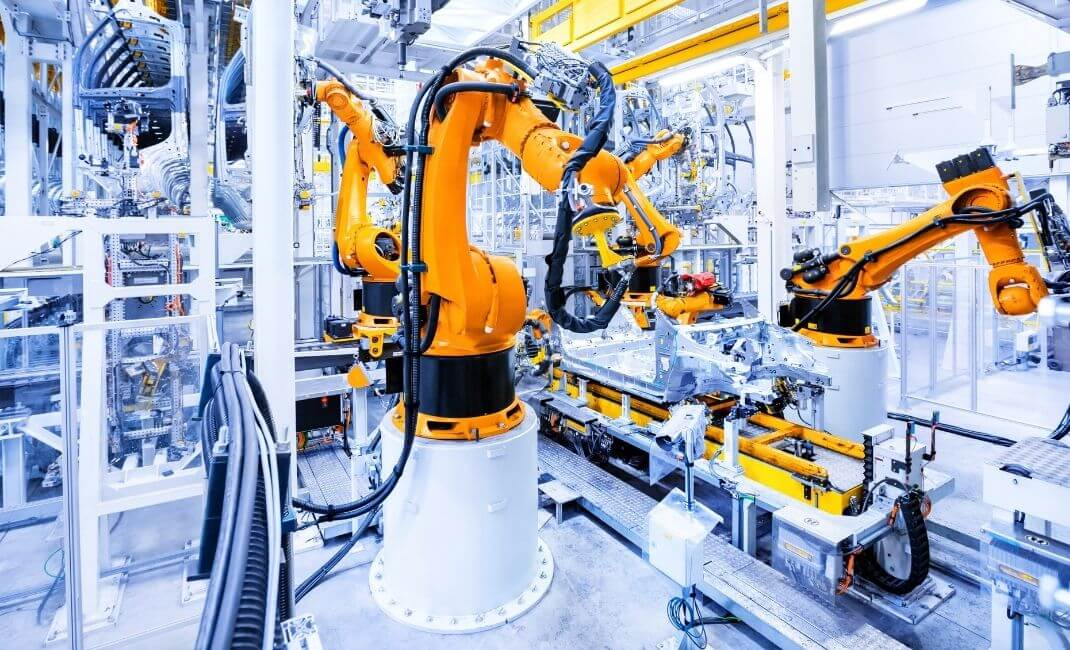
\includegraphics[width=13cm]{figs/automatizacion_industrial.jpg}
  \end{center}
  \caption{\centering Ejemplo de aplicación de automatización industrial.}
  \label{fig:automatizacion_industrial}
\end{figure}

La estructura de un sistema de automatización industrial se puede representar mediante un triángulo jerárquico de cinco niveles como se observa en la imagen ~\ref{fig:esquema_automatizacion}:

\begin{enumerate}
    \item \textbf{Nivel de gestión}: La alta gerencia usa sistemas ERP para controlar y monitorear todos los procesos de la empresa, desde la producción hasta ventas, compras y proyectos, asegurando eficiencia y alineación entre equipos.\cite{niveles_automatizacion_2}.
    \item \textbf{Nivel de operación}: Este nivel está controlado por el sistema MES. Un sistema MES conecta el mundo digital con la producción, permitiendo supervisar, sincronizar cada fase del proceso y monitorear la producción \cite{sistema_MES}. Este sistema integra datos de operaciones, mantenimiento, seguridad, logística y calidad, permitiendo a la gerencia tomar decisiones informadas sobre todo el proceso, desde las materias primas hasta el producto final. \cite{niveles_automatizacion_2}.
    \item \textbf{Nivel supervisor}: Compuesto por un ordenador industrial que utiliza software especializado para el control de procesos. Su principal objetivo es la parametrización y visualización del proceso y suele utilizars el protocolo de de comunicación Ethernet industrial \cite{niveles_automatizacion_1}.
    \item \textbf{Nivel de control}: Incluye dispositivos como PLCs que ejecutan las órdenes del nivel supervisor y controlan directamente la maquinaria en tiempo real. Estos pueden estar conectados a varios dispositivos de E/S y se comunican mediante protocolos industriales \cite{niveles_automatizacion_1}.
    \item \textbf{Nivel de campo}: Constituido por sensores y actuadores que interactúan directamente con el proceso físico conectados al PLC a través de un bus de campo. Los actuadores ejecutan acciones según las instrucciones recibidas normalmente a través de una conexión punto a punto con el PLC. \cite{niveles_automatizacion_1}. 
\end{enumerate}

Esta estructura permite una gestión eficiente y organizada de los procesos industriales, asegurando que cada componente funcione de manera integrada para optimizar la producción. 

\begin{figure} [h!]
  \begin{center}
    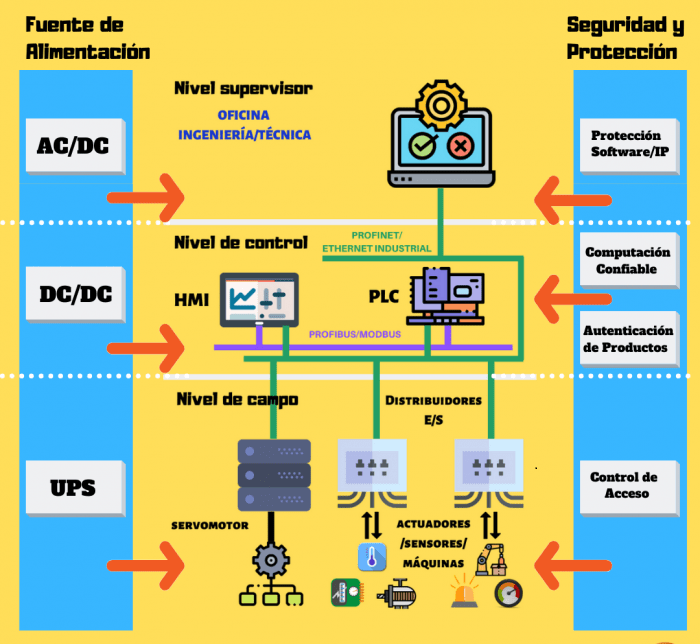
\includegraphics[width=15.5cm]{figs/esquema_automatizacion}
  \end{center}
  \caption{\centering Niveles de la pirámide de automatización. \cite{imagen_niveles_automatizacion}}  
  \label{fig:esquema_automatizacion}
\end{figure}  

\newpage

\subsection{Tipos de automatización industrial}

Los sistemas de automatización industrial se clasifican principalmente en cuatro tipos según su nivel de flexibilidad y aplicación en los procesos productivos:

\begin{enumerate}
    \item \textbf{Automatización fija}: Utilizada en procesos específicos y repetitivos donde no se requieren modificaciones en el diseño del producto debido a que aplicar modificaciones resulta casi imposible. Es ideal para la producción a gran escala de productos estables \cite{tipos_industrial}.
    \item \textbf{Automatización programable}: Aplicada en la fabricación por lotes, permite modificar el proceso mediante reprogramación, aunque esto puede consumir tiempo \cite{tipos_industrial}.
    \item \textbf{Automatización flexible}: Variante más avanzada de la automatización programable, que facilita cambios rápidos y automáticos en la producción sin interrupciones significativas \cite{tipos_industrial}.
    \newpage
    \item \textbf{Sistema Integrado de Automatización}: Conjunto de máquinas, procesos y datos sincronizados bajo un único sistema de control. Integra herramientas como CAD, CAM, robots y sistemas de transporte automatizados para optimizar la producción \cite{tipos_industrial}.
\end{enumerate}

\subsection{Ventajas y desventajas de la automatización industrial}

La automatización industrial ha transformado profundamente los procesos de producción, introduciendo tecnologías avanzadas que permiten aumentar la eficiencia, mejorar la calidad y reducir los costos operativos \cite{des_ventajas_1}. A continuación, se presentan las principales ventajas:

\begin{itemize}

 \item \textbf{Mayor productividad laboral}: La automatización acelera los procesos de producción, permitiendo fabricar más productos con una mejor calidad. Las nuevas tecnologías pueden operar de manera continua sin perder precisión, lo que incrementa la eficiencia y el rendimiento por hora de trabajo  \cite{des_ventajas_1}.

 \item \textbf{Mejora en la calidad del producto}: Uno de los principales beneficios de la automatización es la reducción de la cantidad de unidades defectuosas. Los sistemas automatizados garantizan una mayor uniformidad y precisión en la fabricación, cumpliendo con los estándares de calidad \cite{des_ventajas_2}.
   
\item \textbf{Reducción de costos de producción}: La automatización permite disminuir el gasto en mano de obra al reemplazar tareas repetitivas con maquinaria, lo que reduce el costo unitario de producción. Los sistemas automatizados operan de manera constante, aumentando la eficiencia y proporcionando un alto retorno de inversión al minimizar costos laborales, ausencias y otros gastos operativos \cite{des_ventajas_1}.

\item \textbf{Menos trabajo manual repetitivo}: En muchas industrias, es necesario supervisar constantemente variables como temperatura, presión o nivel de líquidos. Un sistema automatizado permite gestionar estas tareas mediante controladores de lazo cerrado, reduciendo la necesidad de intervención humana en actividades rutinarias \cite{des_ventajas_1}.

\item \textbf{Mayor seguridad}: Al implementar un sistema automatizado, los trabajadores pasan de realizar tareas directamente en el proceso a supervisarlas, lo que disminuye los riesgos laborales. Las máquinas pueden operar en entornos peligrosos o extremos, sustituyendo a los empleados en situaciones de alto riesgo, reduciendo así los accidentes laborales \cite{des_ventajas_2}.

\item \textbf{Facilita la monitorización remota}: Muchas operaciones industriales requieren ser controladas a distancia para una supervisión más eficiente. Los sistemas automatizados permiten la comunicación entre el área de producción y el centro de control, permitiendo a los operadores gestionar los procesos de manera remota \cite{des_ventajas_2}.

\end{itemize}

Sin embargo, junto con estos beneficios, como sucede en cualquier ámbito, también surgen desafíos y limitaciones que deben ser considerados por las empresas antes de implementar estos sistemas. Por eso, seguidamente se muestran algunas desventajas de la automatización industrial:

\begin{itemize}

\item \textbf{Aumento de la contaminación}: Muchas máquinas requieren motores que funcionan con combustibles o productos químicos que pueden generar emisiones contaminantes \cite{des_ventajas_1}.

\item \textbf{Menor flexibilidad}: Una máquina automatizada está diseñada para realizar tareas específicas, lo que limita la capacidad de adaptación a nuevas funciones en comparación con un trabajador humano. Actualmente, ciertas tareas, como el ensamblaje de productos con formas irregulares, siguen dependiendo del trabajo manual \cite{des_ventajas_1}.

\item \textbf{Altos costos de implementación}: La inversión inicial para adoptar un sistema automatizado es elevada. Además de los gastos en investigación y desarrollo, es necesario considerar los costos de mantenimiento, formación del personal y servicio técnico, lo que suma un desafío económico para las empresas que buscan automatizar sus procesos \cite{des_ventajas_2}.
\end{itemize}

\subsection{Equipos para la automatización industrial}

La automatización industrial se apoya en una amplia gama de dispositivos diseñados para controlar, supervisar y optimizar procesos dentro de entornos productivos. Entre estos equipos, destacan los Controladores Lógicos Programables (PLCs) y las Interfaces Hombre-Máquina (HMI), los cuales cumplen un papel fundamental en la implementación y operación de sistemas automatizados modernos.

\subsubsection{Controladores lógicos programables (PLCs)}

Un PLC (Controlador Lógico Programable) es una computadora diseñada específicamente para automatizar procesos industriales. Su tarea principal es controlar de manera eficiente y segura los sistemas que conforman una máquina o proceso, lo cual es clave para el avance tecnológico de las industrias. Estos dispositivos operan mediante un ciclo en el que se realiza un autodiagnóstico, se leen las entradas, se ejecuta el programa y finalmente se actualizan las salidas, lo que les permite adaptarse rápidamente a las condiciones cambiantes del entorno  \cite{plc_info}.

Existen distintos tipos de PLC, cada uno adaptado a las necesidades particulares de cada industria. Entre los más comunes se encuentran los modelos compactos, modulares o de banda estrecha. Marcas como Siemens y Allen Bradley son líderes en este mercado, ofreciendo una amplia variedad de productos y accesorios para mejorar la automatización de los procesos. Los PLCs se usan en una gran variedad de sectores, incluyendo la fabricación de cemento, plásticos, muebles, automotriz, transporte, energía y seguridad, ayudando a mejorar la eficiencia y reducir los costos operativos  \cite{plc_info}.

\begin{figure} [h!]
  \begin{center}
    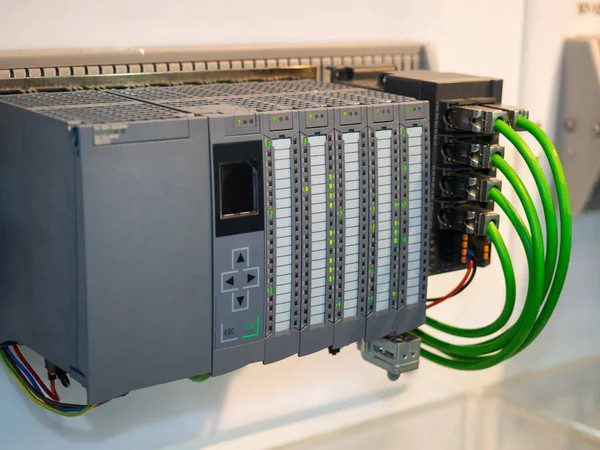
\includegraphics[width=9.5cm]{figs/info_plc}
  \end{center}
  \caption{\centering PLC de la serie Siemens S7-1500.}
  \label{fig:info_plc}
\end{figure} 

Una de las principales características de los PLC es su capacidad para controlar entradas y salidas de manera segura. Además, son compatibles con varios lenguajes de programación, lo que permite su fácil integración con sistemas de supervisión y control. Estos dispositivos pueden ser reprogramados según las necesidades del proceso, lo que les da gran flexibilidad y adaptabilidad en entornos industriales que están en constante cambio  \cite{plc_info}. \\

El lenguaje de programación utilizado para los PLCs y en este proyecto es el lenguaje KOP, también conocido como \textbf{Ladder}. Su popularidad se debe a su antigüedad, disponibilidad, mantenibilidad y facilidad de uso. Diseñado para imitar los diagramas eléctricos tradicionales, permite a técnicos e ingenieros familiarizados con estos esquemas adaptarse fácilmente a la programación en este lenguaje. Su naturaleza gráfica permite una comprensión rápida de la lógica del programa, lo que simplifica el proceso de mantenimiento y resolución de problemas \cite{ladder_info}.

\begin{figure} [h!]
  \begin{center}
    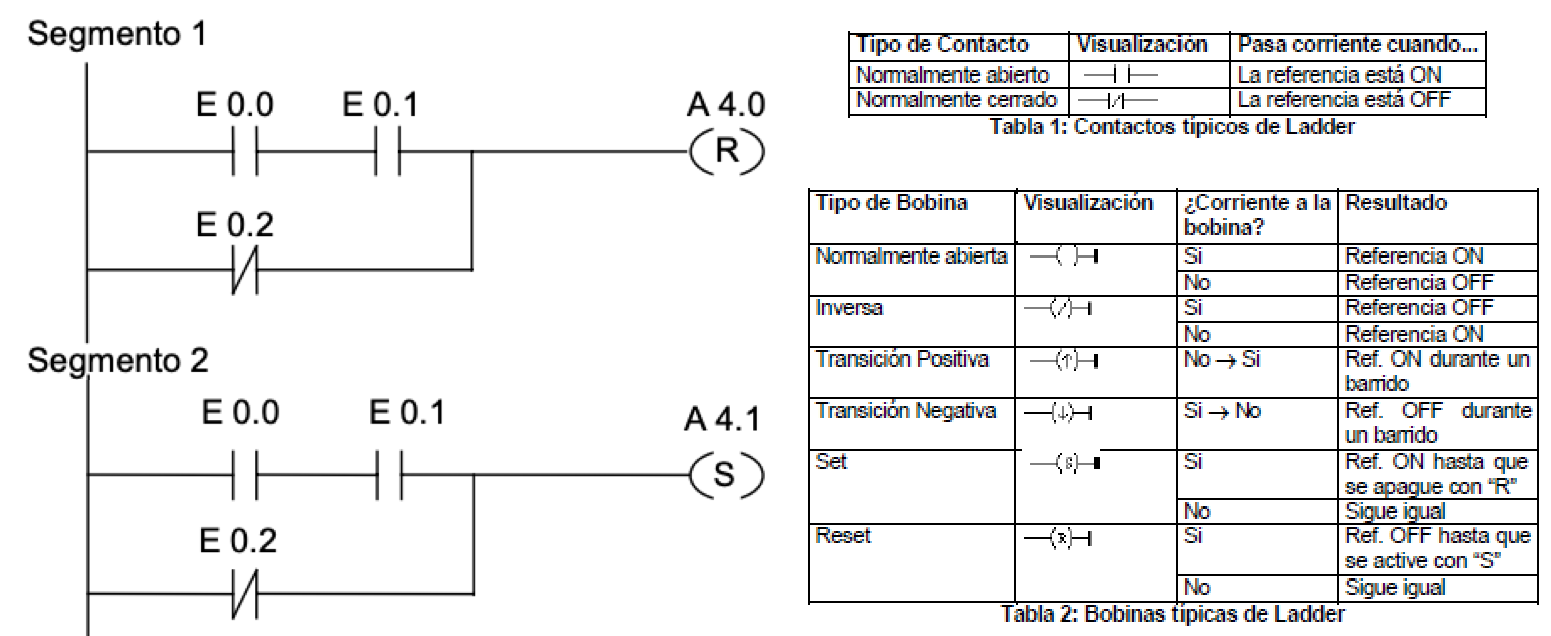
\includegraphics[width=15cm]{figs/ladder}
  \end{center}
  \caption{\centering Ejemplo del lenguaje de programación Ladder.}
  \label{fig:ladder}
\end{figure} 


\subsubsection{Interfaz humano máquina (HMI)}

Una Interfaz Hombre-Máquina (HMI) es un dispositivo que permite a los operarios comunicarse con sistemas automatizados dentro de un entorno industrial. Básicamente, actúa como una pantalla o panel táctil desde el cual se puede supervisar, controlar y ajustar el funcionamiento de una máquina o proceso. Los HMI permiten visualizar datos en tiempo real, como temperaturas, velocidades o estados de operación, y también enviar comandos para modificar parámetros o detener procesos si es necesario \cite{hmi}.

Además, estos dispositivos están pensados para funcionar en condiciones industriales exigentes, con diseños robustos y duraderos \cite{hmi}. También soportan múltiples idiomas y pueden adaptarse a distintos sectores y tipos de máquinas \cite{hmi}. En resumen, un HMI es una herramienta fundamental para mejorar la comunicación entre las personas y los sistemas automatizados, permitiendo un control más intuitivo, rápido y preciso de los procesos industriales.

\begin{figure} [h!]
  \begin{center}
    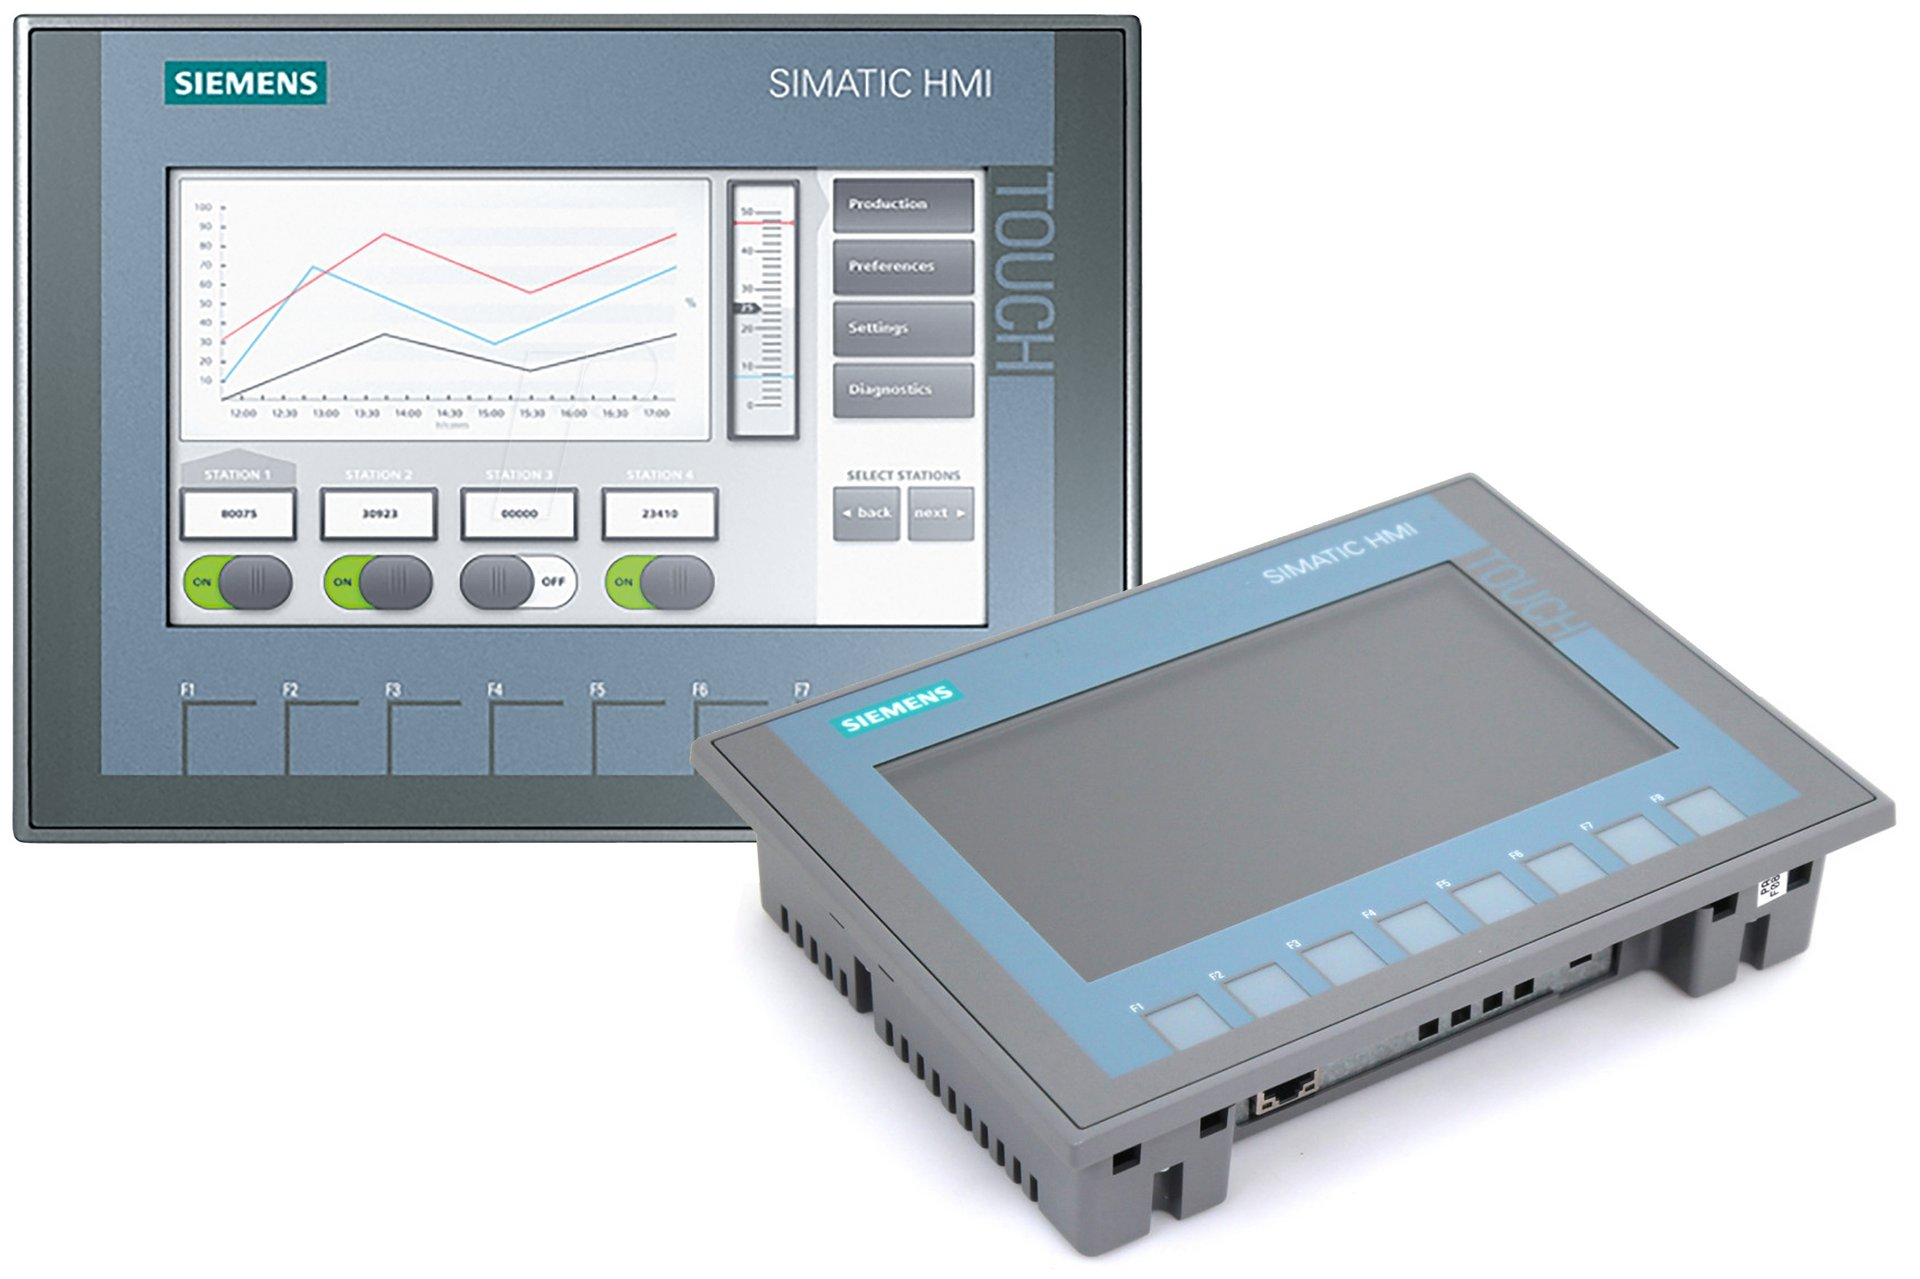
\includegraphics[width=13cm]{figs/HMI}
  \end{center}
  \caption{\centering HMI Siemens.}
  \label{fig:HMI}
\end{figure} 

\section{La robótica}
\label{sec:segundaseccion} % etiqueta para luego referenciar esta sección

La robótica es la disciplina científica que integra conocimientos de electrónica, mecánica e informática para desarrollar sistemas automatizados capaces de realizar tareas de manera autónoma o semiautónoma \cite{definicion_robot}. 

La robótica, en términos generales, abarca el diseño, construcción y programación de sistemas capaces de percibir su entorno, procesar información y ejecutar acciones de manera autónoma \cite{definicion_robot_2}. A diferencia de la robótica industrial, que se centra principalmente en tareas repetitivas, de alta precisión y en entornos estructurados como fábricas, la robótica tradicional se caracteriza por la diversidad de aplicaciones y la necesidad de adaptarse a contextos más variables y no estructurados. Esto implica la utilización de componentes versátiles, diseñados específicamente para cumplir funciones concretas en ámbitos como la robótica móvil, de exploración, educativa o de asistencia personal \cite{definicion_robot_2}.

En estos sistemas, los sensores juegan un papel crucial al proporcionar información del entorno que permite la adaptación del comportamiento del robot. Estos sensores, que pueden medir variables como luz, distancia, posición, velocidad, temperatura o fuerza, actúan como los "sentidos" del sistema robótico, y son fundamentales para su interacción efectiva con entornos complejos y no predecibles \cite{definicion_robot_2}. En contraste, en la robótica industrial los sensores suelen estar optimizados para tareas concretas dentro de procesos controlados y altamente repetitivos, donde las condiciones del entorno apenas varían.

Por su parte, el software y los algoritmos que controlan el comportamiento del robot en la robótica tradicional deben ser especialmente robustos, adaptativos y, en muchos casos, incorporar técnicas de inteligencia artificial o aprendizaje automático \cite{definicion_robot_2}. Esto permite al robot reaccionar de forma flexible a situaciones no previstas, algo menos común en la robótica industrial, donde los algoritmos suelen estar más orientados a la eficiencia, estabilidad y cumplimiento exacto de ciclos de producción \cite{definicion_robot_2}. Finalmente, los actuadores son los responsables de ejecutar las decisiones del sistema de control y deben estar diseñados para responder con precisión y versatilidad, siendo capaces de adaptarse a tareas muy variadas, a diferencia de los actuadores industriales, que suelen estar optimizados para movimientos repetitivos y bien definidos en líneas de montaje automatizadas \cite{definicion_robot_2}.

\begin{figure} [h!]
  \begin{center}
    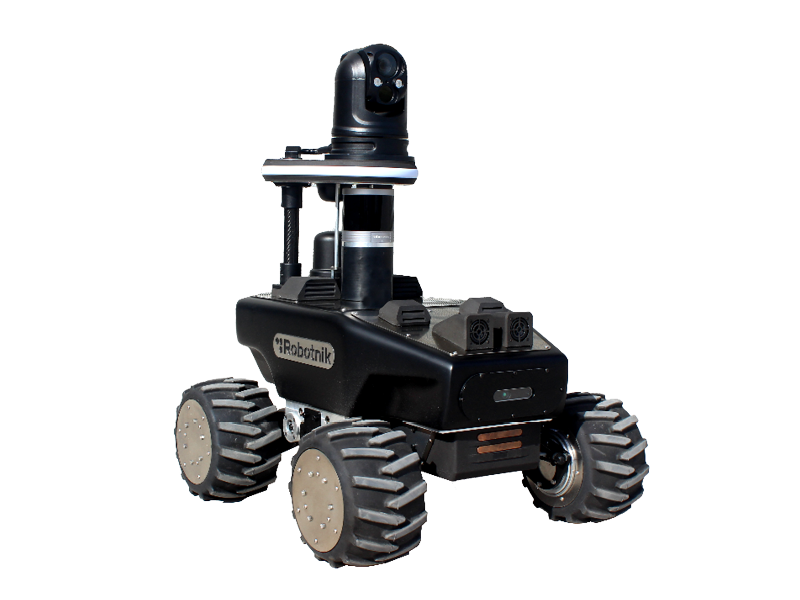
\includegraphics[width=8cm]{figs/Robot_intro}
  \end{center}
  \caption{\centering RB-WATCHER de Robotink.}
  \label{fig:Robot_intro}
\end{figure}

\subsection{Robótica industrial}

Según la norma internacional ISO 8373:2021 un robot industrial se define como ``un manipulador multifuncional, reprogramable y controlado automáticamente, programable en tres o más ejes que puede estar fijo en un área o móvil para su uso en aplicaciones de automatización industrial'' \cite{definicion_iso}. Todo ello a partir de trayectorias variables para ejecutar diversas tareas cíclicas y adaptables. 

La robótica industrial es una disciplina de la ingeniería robótica dedicada al diseño, desarrollo y fabricación de robots industriales con el propósito de automatizar tareas repetitivas tradicionalmente realizadas por seres humanos. Estos sistemas robóticos se caracterizan por seguir una secuencia de instrucciones predefinidas, ejecutando ciclos de trabajo continuos en líneas de producción de diversos sectores industriales. Estos robots son considerados industriales debido a que se utilizan en la industria manufacturera en sectores como la automoción, electrónica, alimentación, farmacéutico... En ellos contribuyen significativamente a mejorar la eficiencia, la velocidad y la calidad de los procesos productivos \cite{info_robotica_industrial_1}. 

A diferencia de los robots de servicio, los robots industriales operan en entornos altamente controlados, lo que simplifica su programación y control. Debido a estas condiciones estables, estos robots suelen tener más de tres grados de libertad, permitiéndoles realizar movimientos complejos con gran precisión. Aunque su aplicación principal ha sido históricamente en entornos industriales, su uso se ha expandido hacia sectores como la minería, la agricultura, el comercio y la salud, demostrando su versatilidad y adaptabilidad. \\

\begin{figure} [h!]
  \begin{center}
    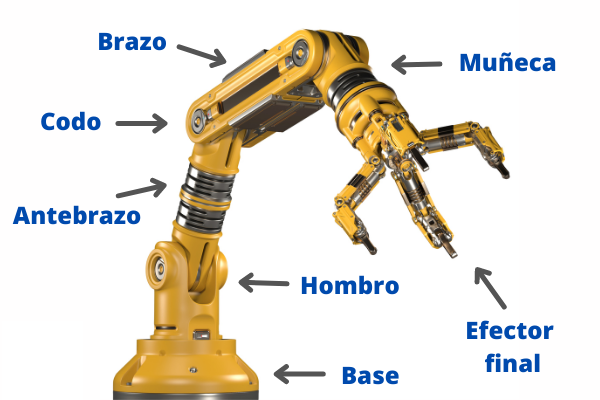
\includegraphics[width=9cm]{figs/brazo_industrial}
  \end{center}
  \caption{\centering Partes de un brazo robótico industrial.}
  \label{fig:brazo_industrials}
\end{figure}

Para que un brazo robótico sea considerado industrial, debe cumplir con una serie de características técnicas y funcionales que lo hagan adecuado para entornos de producción. Entre ellas, destacan la precisión y la repetibilidad, que permiten realizar tareas con tolerancias muy ajustadas. También debe tener una estructura robusta y una capacidad de carga suficiente según la aplicación, así como al menos seis grados de libertad para poder ejecutar movimientos complejos \cite{brazo_industrial}.

Otra característica fundamental es la velocidad de operación, ya que en entornos industriales es clave mantener ritmos de trabajo altos. Además, debe ser fácilmente programable y compatible con sistemas de automatización como PLCs o entornos como ROS, y permitir la integración con sensores, cámaras o herramientas específicas  \cite{brazo_industrial}.

Desde el punto de vista de seguridad y conectividad, debe cumplir con normativas como la ISO 10218 y ser compatible con protocolos industriales como PROFINET o EtherCAT \cite{brazo_industrial}. 

Desde la aparición de los primeros prototipos de robots industriales, ha surgido un debate sobre su impacto en el empleo humano, con preocupaciones respecto a una posible sustitución de la mano de obra. Sin embargo, numerosos estudios sostienen que, lejos de desplazar a los trabajadores, estos sistemas robóticos buscan mejorar las condiciones laborales, eliminando tareas monótonas o peligrosas \cite{info_robotica_industrial_2}. 

\section{Unión entre la automatización y la robótica}
\label{sec:terceraseccion}

Entrando al siglo XXI se desarrollan los primeros robots colaborativos, conocidos como cobots, concebidos para cooperar de manera directa con las personas. Estos dispositivos se caracterizan por su seguridad, adaptabilidad y facilidad de programación, convirtiéndose en una solución ideal para entornos industriales donde es necesario combinar tareas manuales y automatizadas  \cite{intro_union}. 

En los años 2010, la Industria 4.0 emergió como una nueva fase en la manufactura, caracterizada por la digitalización y la interconexión de sistemas de producción.  Los robots industriales se convirtieron en componentes clave de las fábricas inteligentes, colaborando estrechamente con humanos y otros sistemas automatizados para optimizar la eficiencia y la flexibilidad en la producción \cite{intro_union}. 

\subsection{Comunicaciones entre los dispositivos}

Las comunicaciones entre dispositivos industriales son fundamentales para que los procesos de producción actuales funcionen de forma segura, eficiente y automatizada \cite{intro_com}. Gracias a ellas, sensores, actuadores, controladores y sistemas de gestión pueden intercambiar datos constantemente, asegurando que todo el proceso esté coordinado y optimizado. El objetivo principal de estas comunicaciones es transformar la información captada del entorno en datos útiles que faciliten la toma de decisiones rápidas y eficaces \cite{intro_com}. Esto no solo mejora la eficiencia de la producción, sino que también ayuda a prevenir errores, optimizar el uso de recursos y mantener los procesos en marcha sin interrupciones. A diferencia de las redes convencionales, las comunicaciones industriales deben cumplir con requisitos muy exigentes: alta fiabilidad, resistencia a condiciones adversas, capacidad para operar en tiempo real y determinismo. \cite{intro_com}. 

La tecnología de \textbf{bus de campo} apareció a finales de los años 80 con el objetivo de ofrecer un método estandarizado para conectar múltiples dispositivos de campo en entornos industriales. El bus de campo es una red de comunicación industrial bidireccional y multipunto que conecta dispositivos de campo inteligentes, sustituyendo los sistemas de control centralizados por redes distribuidas \cite{info_bus}. Existen múltiples variantes desarrolladas por fabricantes para diferentes nichos destacando: PROFIBUS en automoción y control de procesos, CANbus en el sector automotriz y maquinaria y Foundation Fieldbus en industrias de petróleo y gas entre otros \cite{bus_vs_ethernet}.

\begin{figure} [h!]
  \begin{center}
    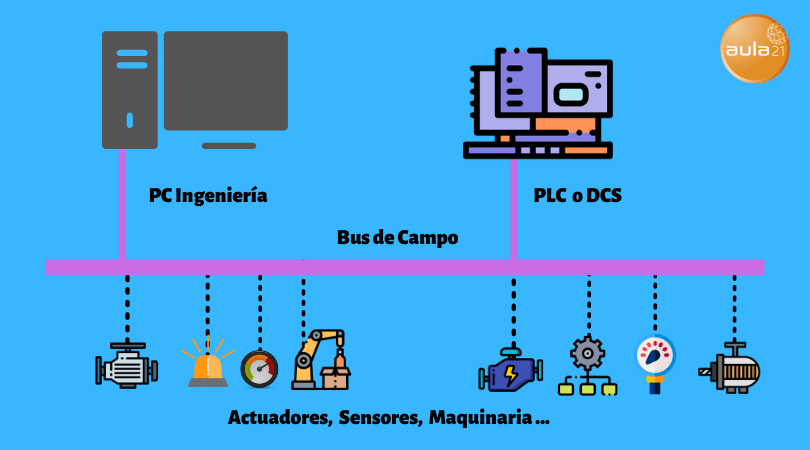
\includegraphics[width=15cm]{figs/bus_de_campo}
  \end{center}
  \caption{\centering Ejemplo básico de dus de campo. \cite{info_bus}}
  \label{fig:bus_de_campo}
\end{figure} 

Por otro lado, la tecnología \textbf{Ethernet industrial} surge como una evolución de Ethernet tradicional, adaptándose a los estrictos requerimientos de entornos industriales donde la robustez, el intercambio de datos en tiempo real y la resistencia a interferencias son esenciales. A partir del estándar IEEE 802.3, Ethernet industrial integra mejoras específicas para la automatización, soportando protocolos como Modbus TCP/IP, PROFINET y EtherCAT \cite{bus_vs_ethernet}.

Entre sus principales ventajas frente a los sistemas de bus de campo tradicionales destacan sus altas velocidades de comunicación (desde 10 Mbps hasta 10 Gbps), su apertura e interoperabilidad, la escalabilidad de la red y su rentabilidad. Estas características permiten su uso tanto en el monitoreo en tiempo real como en la integración de sistemas de gestión y supervisión de plantas industriales, convirtiéndolo en la base de las redes industriales modernas \cite{bus_vs_ethernet}.

\begin{figure} [h!]
  \begin{center}
    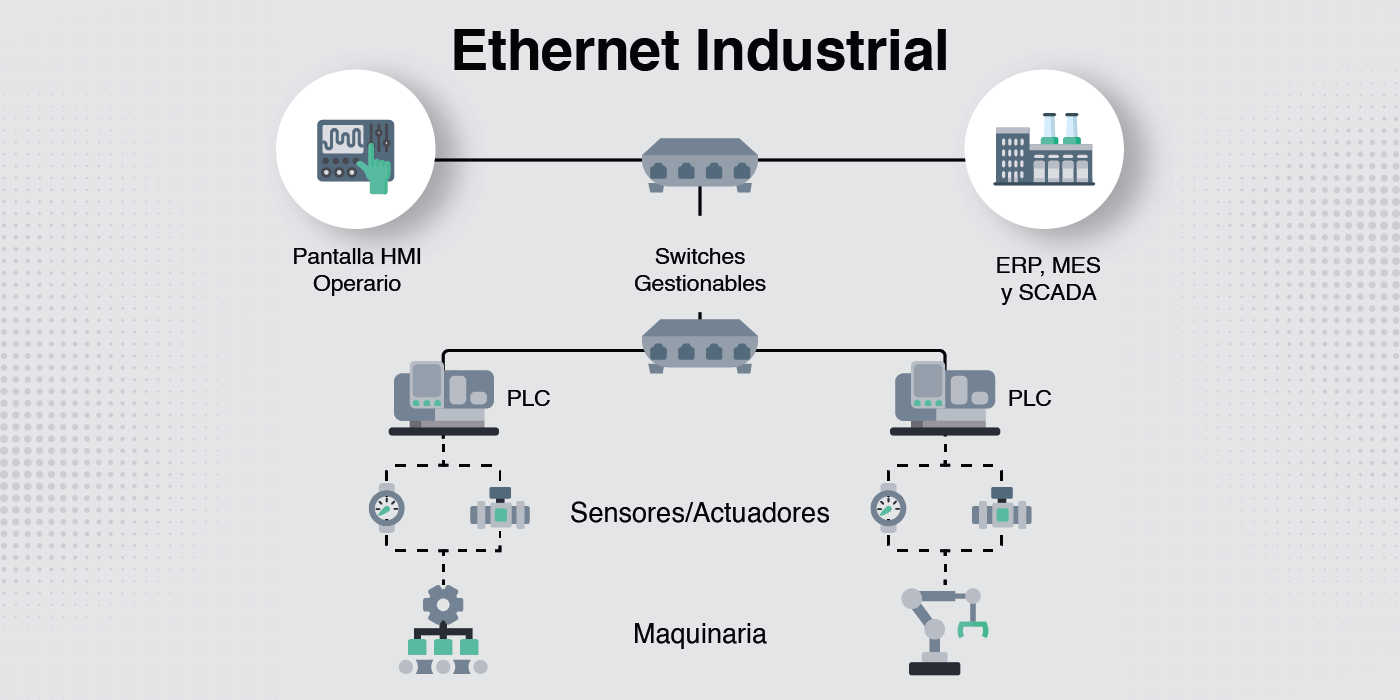
\includegraphics[width=15.5cm]{figs/ethernet_industrial}
  \end{center}
  \caption{\centering Ejemplo básico de red de ethernet industrial. \cite{ethernet_imagen}}
  \label{fig:ethernet_industrial}
\end{figure} 


\subsection{Metodología de la automatización industrial}

En la automatización industrial, es fundamental seguir una metodología clara que permita diseñar, implementar y controlar los procesos de forma ordenada y eficiente. Para ello, existen herramientas y enfoques que ayudan a representar el comportamiento del sistema, identificar sus distintos modos de funcionamiento y supervisar su estado en tiempo real.

Una de las herramientas más utilizadas es el GRAFCET, un lenguaje gráfico que permite describir de forma sencilla el funcionamiento secuencial de un sistema. Junto a él, la guía GEMMA ayuda a identificar los distintos modos de operación del sistema (como arranque, parada o fallo), y sirve como complemento al GRAFCET para organizar mejor el control general del proceso. Por último, los sistemas SCADA juegan un papel clave en la supervisión de procesos industriales, permitendo al operador visualizar en tiempo real lo que ocurre en planta, modificar parámetros y detectar posibles errores de forma rápida.

\newpage

\subsubsection{GRAFCET}

El modelo GRAFCET (Graphe Fonctionnel de Commande Étape Transition) es un método gráfico que se utiliza en la automatización industrial para representar y controlar procesos secuenciales. Creado en 1977 por la AFCET (Asociación Francesa para la Cibernética Económica y Técnica), su objetivo es describir el comportamiento de los sistemas de control mediante un diagrama de etapas y transiciones \cite{grafcet_info}. Esto no es un lenguaje de programación, sino una forma de resolver el problema de automatización secuencial previo a su programación en el PLC. A continuación, se describen los distintos elementos que conforman un GRAFCET:

\begin{enumerate}
    \item \textbf{Etapas}: Se representan como cuadros numerados en el diagrama. Cada etapa indica un estado específico del sistema y las acciones que deben llevarse a cabo cuando esa etapa está activa. La etapa inicial se representa con un doble cuadrado.
    \item \textbf{Transiciones}: Son las condiciones que deben cumplirse para que el sistema pase de una etapa a otra. Estas condiciones se representan por líneas que cruzan de manera perpendicular las etapas. Las transiciones se activan cuando se cumple una condición lógica, como el final de un proceso o la llegada de una señal.
    \item \textbf{Uniones}: Representan las conexiones entre varias etapas y permiten que se ejecuten acciones simultáneas en diferentes partes del sistema. Las uniones facilitan la ejecución de procesos en paralelo.
    \item \textbf{Acciones}: Son las operaciones que se realizan cuando una etapa está activa. Estas acciones están directamente vinculadas a la etapa correspondiente.
\end{enumerate}
    
Este modelo resulta muy útil en procesos industriales donde las operaciones siguen una secuencia lógica y estructurada. Se utiliza comúnmente en la programación de PLCs (Controladores Lógicos Programables), ya que permite controlar sistemas paso a paso y asegura que las acciones se realicen de manera secuencial \cite{grafcet_info}.

\begin{figure} [h!]
  \begin{center}
    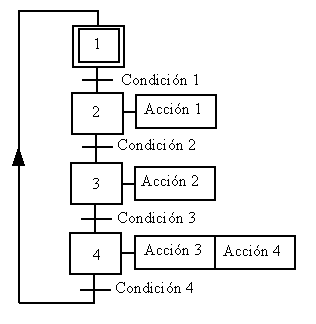
\includegraphics[width=8cm]{figs/grafcet_def}
  \end{center}
  \caption{\centering Ejemplo básico de GRAFCET.}
  \label{fig:grafcet_def}
\end{figure} 

Una vez creado el Grafcet, para poder introducir la lógica pensada en el PLC, hay que traducir la información al lenguaje ladder, que es el cual entiende el PLC. Para ello se deben asignar direcciones de memoria en el PLC a cada etapa, entradas, salidas y demás elementos como contadores o temporizadores. Una vez traducido el Grafcet al lenguaje Ladder e introducido en el PLC ya se puede ejecutar la secuencia realizada del sistema.

\subsubsection{Guia GEMMA}

La Guía GEMMA (Guía para la Elaboración de los Modelos de los Modos de Marcha y Parada de una Automatización) es una metodología utilizada en el ámbito de la automatización industrial para representar de forma clara y estructurada los diferentes modos de funcionamiento de una máquina o sistema  \cite{guia_gemma}. La guía GEMMA está compuesta por bloques que representan cada uno de estos modos y sus posibles transiciones, lo que proporciona una visión global y ordenada del comportamiento del sistema  \cite{guia_gemma}.

El núcleo de la guía se basa en tres grandes categorías: funcionamiento, parada o puesta en marcha, y defecto. En cada categoría se pueden identificar varios subestados como:

\begin{itemize}
  \item  \textbf{Funcionamiento}: La producción en curso o marcha de cierre \cite{guia_gemma}.
  \item \textbf{Parada o puesta en marcha}: La parada al estado inicial o de final de ciclo \cite{guia_gemma}.
  \item \textbf{Defecto}: La parada de emergencia \cite{guia_gemma}. 
\end{itemize} 

Además de su valor como herramienta de planificación, GEMMA se integra fácilmente con otras metodologías como el GRAFCET, permitiendo diseñar automatismos más seguros y eficientes. Al normalizar los distintos modos de operación y facilitar la interpretación de los estados de una automatización, la Guía GEMMA se ha convertido en un recurso esencial para la automatización de procesos.

\begin{figure} [h!]
  \begin{center}
    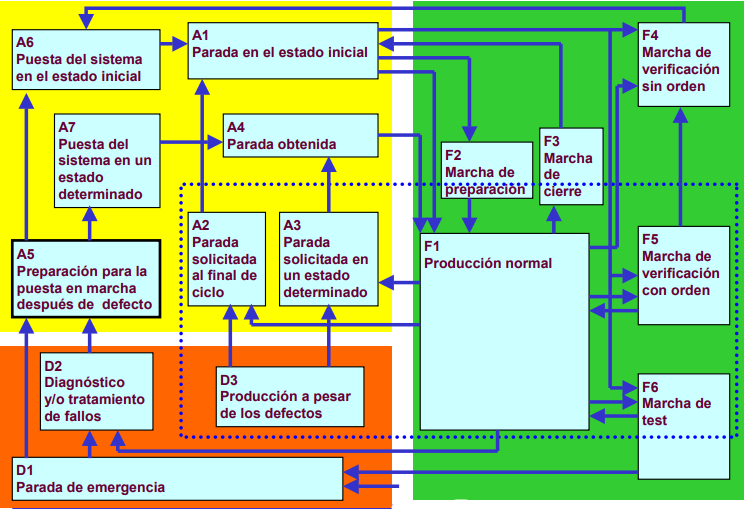
\includegraphics[width=15cm]{figs/guia_gemma}
  \end{center}
  \caption{\centering Ejemplo de guía gemma complejo. \cite{guia_gemma}}
  \label{fig:guia_gemma}
\end{figure} 

\subsubsection{Sistemas SCADA}

Un sistema SCADA (Supervisory Control and Data Acquisition) es una herramienta clave en la automatización industrial, diseñada para supervisar y controlar procesos a distancia mediante la recopilación y análisis de datos en tiempo real \cite{scada}. Estos sistemas permiten monitorear variables críticas como temperatura, presión o caudal, facilitando una operación eficiente y segura de plantas industriales, líneas de producción, redes eléctricas o infraestructuras inteligentes \cite{scada}.

Los sistemas SCADA recopilan información a través de sensores y dispositivos conectados a una red de comunicaciones, ya sea cableada o inalámbrica. Esta información se procesa en un software especializado que permite visualizar los datos, generar alarmas ante anomalías y controlar equipos de forma remota \cite{scada}. Entre sus funciones principales se incluyen la monitorización en tiempo real, análisis de datos, generación de alertas y control de dispositivos como válvulas o motores \cite{scada}.

\begin{figure} [h!]
  \begin{center}
    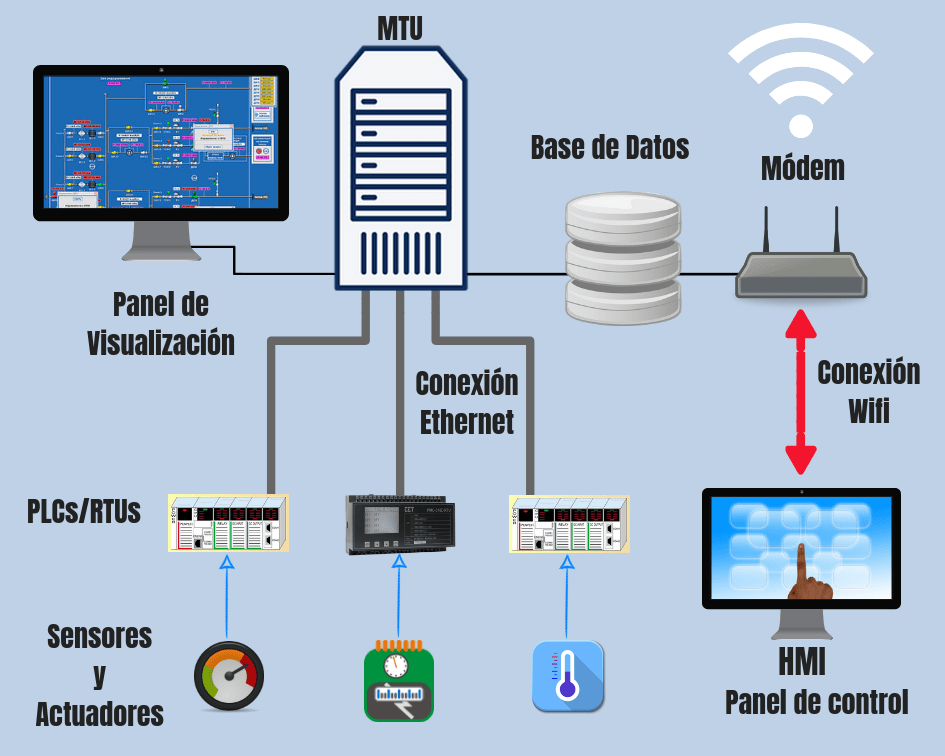
\includegraphics[width=15cm]{figs/SCADA}
  \end{center}
  \caption{\centering Ejemplo de un diagrama básico con sistema SCADA. \cite{scada_img}}
  \label{fig:SCADA}
\end{figure} 

Existen diferentes tipos de sistemas SCADA según su arquitectura: centralizados, donde todos los componentes están en una misma ubicación; distribuidos, con componentes separados conectados por una red; y híbridos, que combinan características de ambos \cite{scada}. Implementar un sistema SCADA adecuado puede mejorar significativamente la eficiencia operativa y la capacidad de respuesta ante incidencias en entornos industriales.

\section{Motivación del trabajo}
\label{sec:cuartaseccion}

La automatización industrial representa una opción laboral muy atractiva, con la transformación digital impulsada por la Industria 4.0 y el auge de tecnologías como el Internet de las Cosas (IoT), la robótica o la inteligencia artificial, la demanda de profesionales cualificados en este ámbito no ha dejado de crecer. Sectores como la automoción, la alimentación o la logística están apostando cada vez más por la automatización para mantenerse competitivos en un mercado globalizado.

\newpage

\begin{figure} [h!]
  \begin{center}
    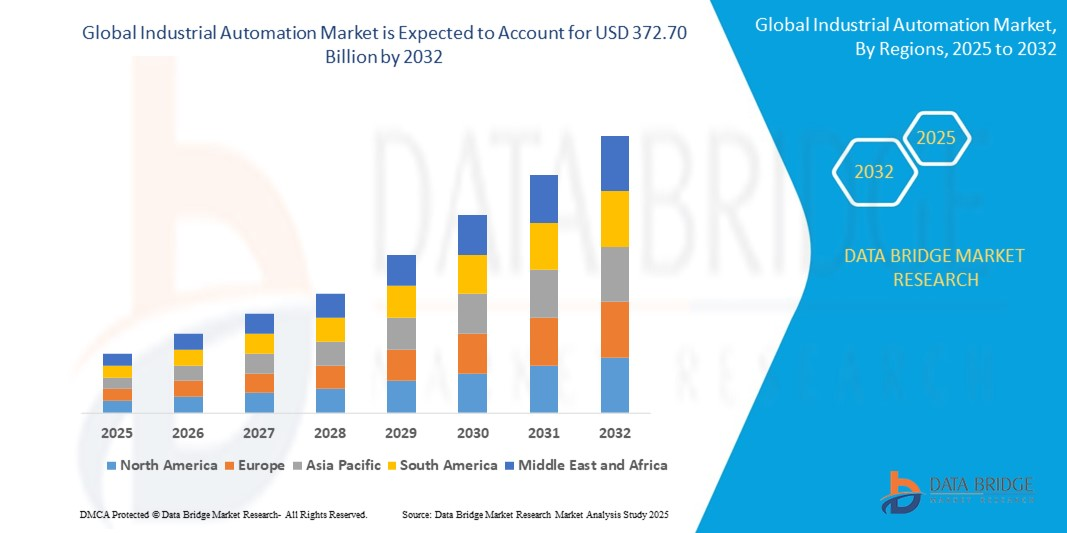
\includegraphics[width=15cm]{figs/grafico_futuro}
  \end{center}
  \caption{\centering Tendencias del mercado global de automatización industrial. \cite{grafico_empleabilidad}}
  \label{fig:grafico_futuro}
\end{figure} 

Como se observa en la figura  ~\ref{fig:grafico_futuro}, se preveé que cada año se invierta más dinero en la automatización industrial,
por lo que este campo tiene un gran futuro. La producción industrial en masa seguirá siendo clave para satisfacer la demanda del mercado, impulsada por el crecimiento demográfico y el alto nivel de consumo. Por otro lado, el desarrollo continuo de nuevas tecnologías y robots hace que el sector esté en constante evolución, tal y como viene ocurriendo desde sus orígenes en la década de 1940.

La creciente escasez de perfiles especializados en el ámbito de la automatización y la robótica incrementa notablemente las oportunidades laborales para quienes cuentan con formación en estas áreas. La familiaridad con simuladores durante la etapa académica puede representar un valor añadido en los procesos de selección, al proporcionar una ventaja comparativa frente a candidatos sin experiencia práctica con sistemas físicos. A ello se suma la existencia de salarios de entrada competitivos, que tienden a incrementarse con la experiencia y que, en general, permiten acceder a una buena calidad de vida.

El trabajo tiene como objetivo el desarrollo de una aplicación basada en el uso de dos simuladores didácticos, concebida como una herramienta de apoyo para facilitar el aprendizaje de contenidos relacionados con la robótica y la automatización. La utilización de este tipo de recursos permite fomentar un aprendizaje más interactivo y dinámico, lo cual contribuye a una mayor motivación del alumnado y a una mejor asimilación de los conceptos teóricos. Asimismo, la combinación de entornos virtuales con prácticas reales constituye una estrategia eficaz para reforzar la formación técnica y preparar al estudiante para los desafíos propios del ámbito profesional.

A lo largo de la formación académica de los ingenieros, se adquieren conocimientos en diferentes disciplinas, tanto desde el punto de vista teórico como práctico. Una característica común en numerosas asignaturas es la utilización de simuladores, los cuales permiten aplicar los conocimientos adquiridos en entornos virtuales controlados. Estos entornos ofrecen múltiples ventajas, entre las que se incluyen la posibilidad de programar sin riesgo de dañar un robot físico, la personalización del entorno de trabajo en función de la aplicación deseada, y la experimentación con distintas configuraciones de forma sencilla y sin incurrir en costes adicionales.

Aun así, trabajar solo con simuladores no es lo mismo que hacerlo con sistemas reales. La experiencia práctica que se obtiene al enfrentarse a un entorno físico es mucho más rica y completa. En la realidad, hay que lidiar con errores de sensores, fallos en los actuadores, problemas mecánicos o situaciones imprevistas que obligan a pensar y reaccionar. Estas experiencias ayudan a desarrollar habilidades muy valiosas, como la capacidad de resolver problemas, tomar decisiones rápidas y adaptarse a los cambios, cosas que un simulador, por muy avanzado que sea, no siempre puede ofrecer.


\chapter{Objetivos}
\label{cap:capitulo2}

\begin{flushright}
\begin{minipage}[]{10cm}
\emph{La automatización bien aplicada no es una amenaza, sino una oportunidad para rediseñar el trabajo, mejorar la productividad y humanizar la industria}\\
\end{minipage}\\

Peter F. Drucker, \textit{ Management: Tasks, Responsibilities, Practices}\\
\end{flushright}

\vspace{1cm}

Tras haber contextualizado en el capítulo anterior los fundamentos de la automatización industrial y su relación con la robótica colaborativa, en esta sección se abordará el problema específico que se pretende resolver con este Trabajo Fin de Grado. Se definirá con precisión el objetivo principal del proyecto, centrado en la automatización de una línea de producción didáctica, y se establecerán las bases sobre las que se desarrollará la solución propuesta. Esta descripción permitirá entender el enfoque adoptado y servirá como punto de partida para detallar los requisitos, las competencias aplicadas y la metodología empleada en el desarrollo del sistema.

\section{Descripción del problema}
\label{sec:descripcion}

El objetivo principal de este Trabajo Fin de Grado es automatizar una línea de producción robotizada utilizando estaciones didácticas de Festo, incorporando un robot colaborativo (UR5e) y estableciendo un sistema de comunicaciones eficiente entre los distintos elementos que componen la celda. Se pretende lograr una integración realista y funcional que sirva tanto como entorno de pruebas para prácticas docentes como demostrador de capacidades en automatización industrial y robótica colaborativa.

Este desarrollo se centra en mejorar la interacción entre los diferentes componentes del sistema (PLCs, HMIs y cobot), garantizando una comunicación fluida y segura, así como un control intuitivo y robusto de todo el proceso productivo.

\section{Requisitos}
\label{sec:requisitos}

Durante el desarrollo del proyecto, se han definido y alcanzado los siguientes requisitos técnicos y funcionales:

\begin{itemize}
	\item Automatización del funcionamiento de las estaciones didácticas (distribución y unión) mediante programación en TIA Portal.

	\item Diseño y configuración de una interfaz HMI para el control del sistema y visualización de estados.

	\item Integración del robot colaborativo UR5e en el flujo de trabajo automatizado, realizando tareas de paletizado.

	\item Creación de una red de comunicaciones PROFINET entre PLCs, HMI y cobot, asegurando el intercambio de datos en tiempo real.

	\item Implementación de lógica de control secuencial utilizando Grafcet y guía GEMMA como base metodológica.

	\item Montaje, conexionado y validación del sistema completo en condiciones reales de funcionamiento.
\end{itemize}

\section{Competencias}
\label{sec:competencias}

Las competencias desarrolladas y aplicadas en este proyecto están contenidas dentro del grado en Ingeniería Robótica Software, y en particular con las asignaturas de robótica industrial, redes de ordenadores, y la asignatura propia de trabajo de fin de grado. A continuación se enumeran las competencias adquiridas:

\begin{itemize}
	\item Se han aplicado los conocimientos adquiridos de forma profesional, resolviendo problemas y elaborando argumentos dentro del ámbito de la robótica. Se ha demostrado capacidad para comunicar información, ideas y soluciones a públicos especializados y no especializados, y se ha fomentado la autonomía en el aprendizaje. Todo ello ha culminado en la realización y defensa de un proyecto que integra y sintetiza las competencias del grado.

	\item Capacidad de diseñar y programar sistemas en red aplicando conceptos de arquitectura de red, protocolos e interfaces de comunicaciones.

	\item Capacidad de diseñar, planificar y programar sistemas de manipulación robóticos.

	\item Capacidad de diseñar robots y sistemas inteligentes atendiendo a los elementos de sensorización y actuación más adecuados dependiendo de la aplicación, los requerimientos del sistema y las condiciones del entorno.

\end{itemize}
 
\section{Metodología}
\label{sec:metodologia}

El desarrollo del presente trabajo se ha basado en una metodología estructurada y secuencial, orientada a la automatización industrial y fundamentada en los estándares Grafcet y Guía GEMMA, los cuales ya fueron explicados en el capítulo 1.

Para definir el comportamiento lógico del sistema automatizado, se utilizó el modelo GRAFCET, que permitió representar de forma clara y estructurada la secuencia de funcionamiento de cada estación, identificando las diferentes etapas del proceso, las transiciones entre ellas basadas en condiciones lógicas, y las acciones asociadas a cada estado. Después se procedió a su traducción al lenguaje Ladder para su implementación en los PLCs. De forma complementaria, se empleó la Guía GEMMA para estructurar los distintos modos de operación del sistema, incluyendo funcionamiento normal, parada, arranque y gestión de fallos, lo que permitió definir una lógica de control más robusta y segura, especialmente ante condiciones anómalas o situaciones de emergencia.

Respecto a la programación del cobot UR5e, se empleó una metodología centrada en la programación mediante la interfaz gráfica PolyScope y ayudándose de la herramienta de paletizado de esta. Una vez desarrollada la lógica, se trasladó directamente al entorno físico y se integró con las estaciones didácticas utilizando comunicación PROFINET.

\section{Plan de trabajo}
\label{sec:plantrabajo}

El desarrollo del proyecto comenzó con la instalación del primer PLC y la interfaz HMI, así como su correspondiente configuración en el entorno TIA Portal. A continuación, se procedió a la instalación de la estación de distribución, realizando el conexionado de todas las entradas y salidas al PLC para su control. Una vez completada esta etapa, se inició la programación de la lógica de control de dicha estación en el PLC y el diseño de la interfaz gráfica del HMI, una fase que se extendió durante aproximadamente un mes hasta alcanzar un funcionamiento completo y estable.

Finalizada la primera estación, se abordó la instalación del segundo PLC y de la estación unión, los cuales se integraron en el mismo proyecto de TIA Portal y se añadieron a la red PROFINET común, permitiendo así la comunicación entre todos los dispositivos del sistema. Del mismo modo, se conectaron las entradas y salidas de la estación de unión, y se comenzó con la programación de su lógica de control. Transcurrido otro mes de trabajo, ambas estaciones estaban totalmente automatizadas y operativas. En esta fase también se implementó la comunicación entre los dos PLCs, permitiendo así una coordinación eficiente que dio lugar a un proceso automatizado conjunto.

Finalmente, una vez completada la automatización de las estaciones, se procedió a la programación del robot colaborativo UR5e. Se desarrolló una secuencia de paletizado de cartones de leche, manipulados mediante una pinza hidráulica capaz de apilar hasta cuatro capas. Una vez definida la secuencia de trabajo del cobot, este fue incorporado a la red PROFINET del sistema, permitiendo su comunicación directa con los PLCs. Se implementó el intercambio de señales de control entre el UR5e y los controladores, integrando al robot dentro del mismo ciclo de operación automatizada. Esta última fase requirió aproximadamente un mes adicional.




\chapter{Plataforma de desarrollo}
\label{cap:capitulo3}

\begin{flushright}
\begin{minipage}[]{10cm}
\emph{Cualquier cosa que pueda ser automatizada, será automatizada..}\\
\end{minipage}\\

Robert Cannon\\
\end{flushright}

\vspace{1cm}

En este capítulo se detallan los recursos hardware y software empleados para llevar a cabo el desarrollo de la aplicación. A nivel hardware, se han utilizado dos maquetas didácticas de automatización industrial del fabricante FESTO, cada una equipada con un PLC y una interfaz HMI común de SIEMENS y un brazo robótico colaborativo de la empresa Universal Robots (UR). En cuanto al software, se han utilizado distintos entornos de desarrollo específicos para cada dispositivo: el software TIA Portal para la programación de los PLCs y la configuración de la HMI, y la plataforma URSim para la simulación y control del brazo robótico. Además, se han empleado librerías propias de los fabricantes, sistemas operativos compatibles con las herramientas utilizadas y conexiones mediante protocolos estándar de comunicación industrial como Profinet. También se ha realizado el montaje completo y el conexionado de todos los elementos.

\section{Estación distribución}

La estación de distribución con cinta transportadora de Festo Didactic \footnote{Image retrieved from Festo.com. (N.d.). Retrieved June 4, 2025, from \url{https://www.festo.com/es/es/p/estacion-de-distribucion-id_PROD_DID_8034566/}} es un módulo del sistema MPS (Modular Production System) que simula una parte de una línea de producción automatizada. Su función principal es clasificar, alinear y transportar piezas de trabajo desde un punto de alimentación hacia otras estaciones del sistema \cite{estacion_distribucion}. Este sistema está diseñado para la formación técnica en automatización industrial, permitiendo a estudiantes aprender a manejar sensores, actuadores, sistemas neumáticos, cintas transportadoras y PLCs. \\

\begin{figure} [h!]
  \begin{center}
    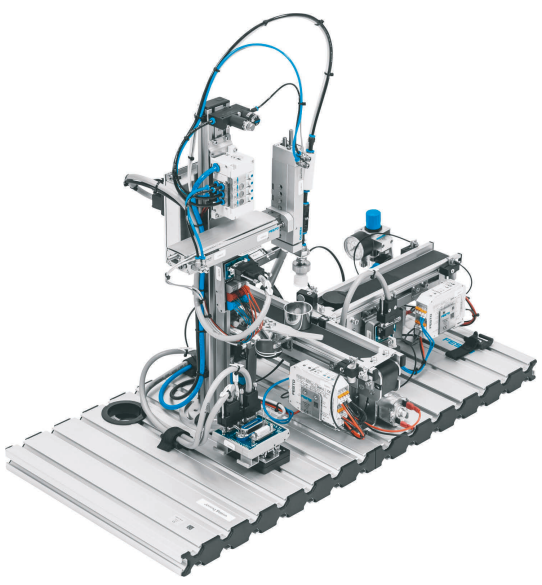
\includegraphics[width=12.5cm]{figs/estacion_distribucion_1}
  \end{center}
  \caption{\centering Estación distribución. \cite{estacion_distribucion}}
  \label{fig:estacion_distribucion_1}
\end{figure} 

En la tabla \ref{fig:estacion_distribucion_3} se detallan las características generales del sistema:

\begin{figure} [h!]
  \begin{center}
    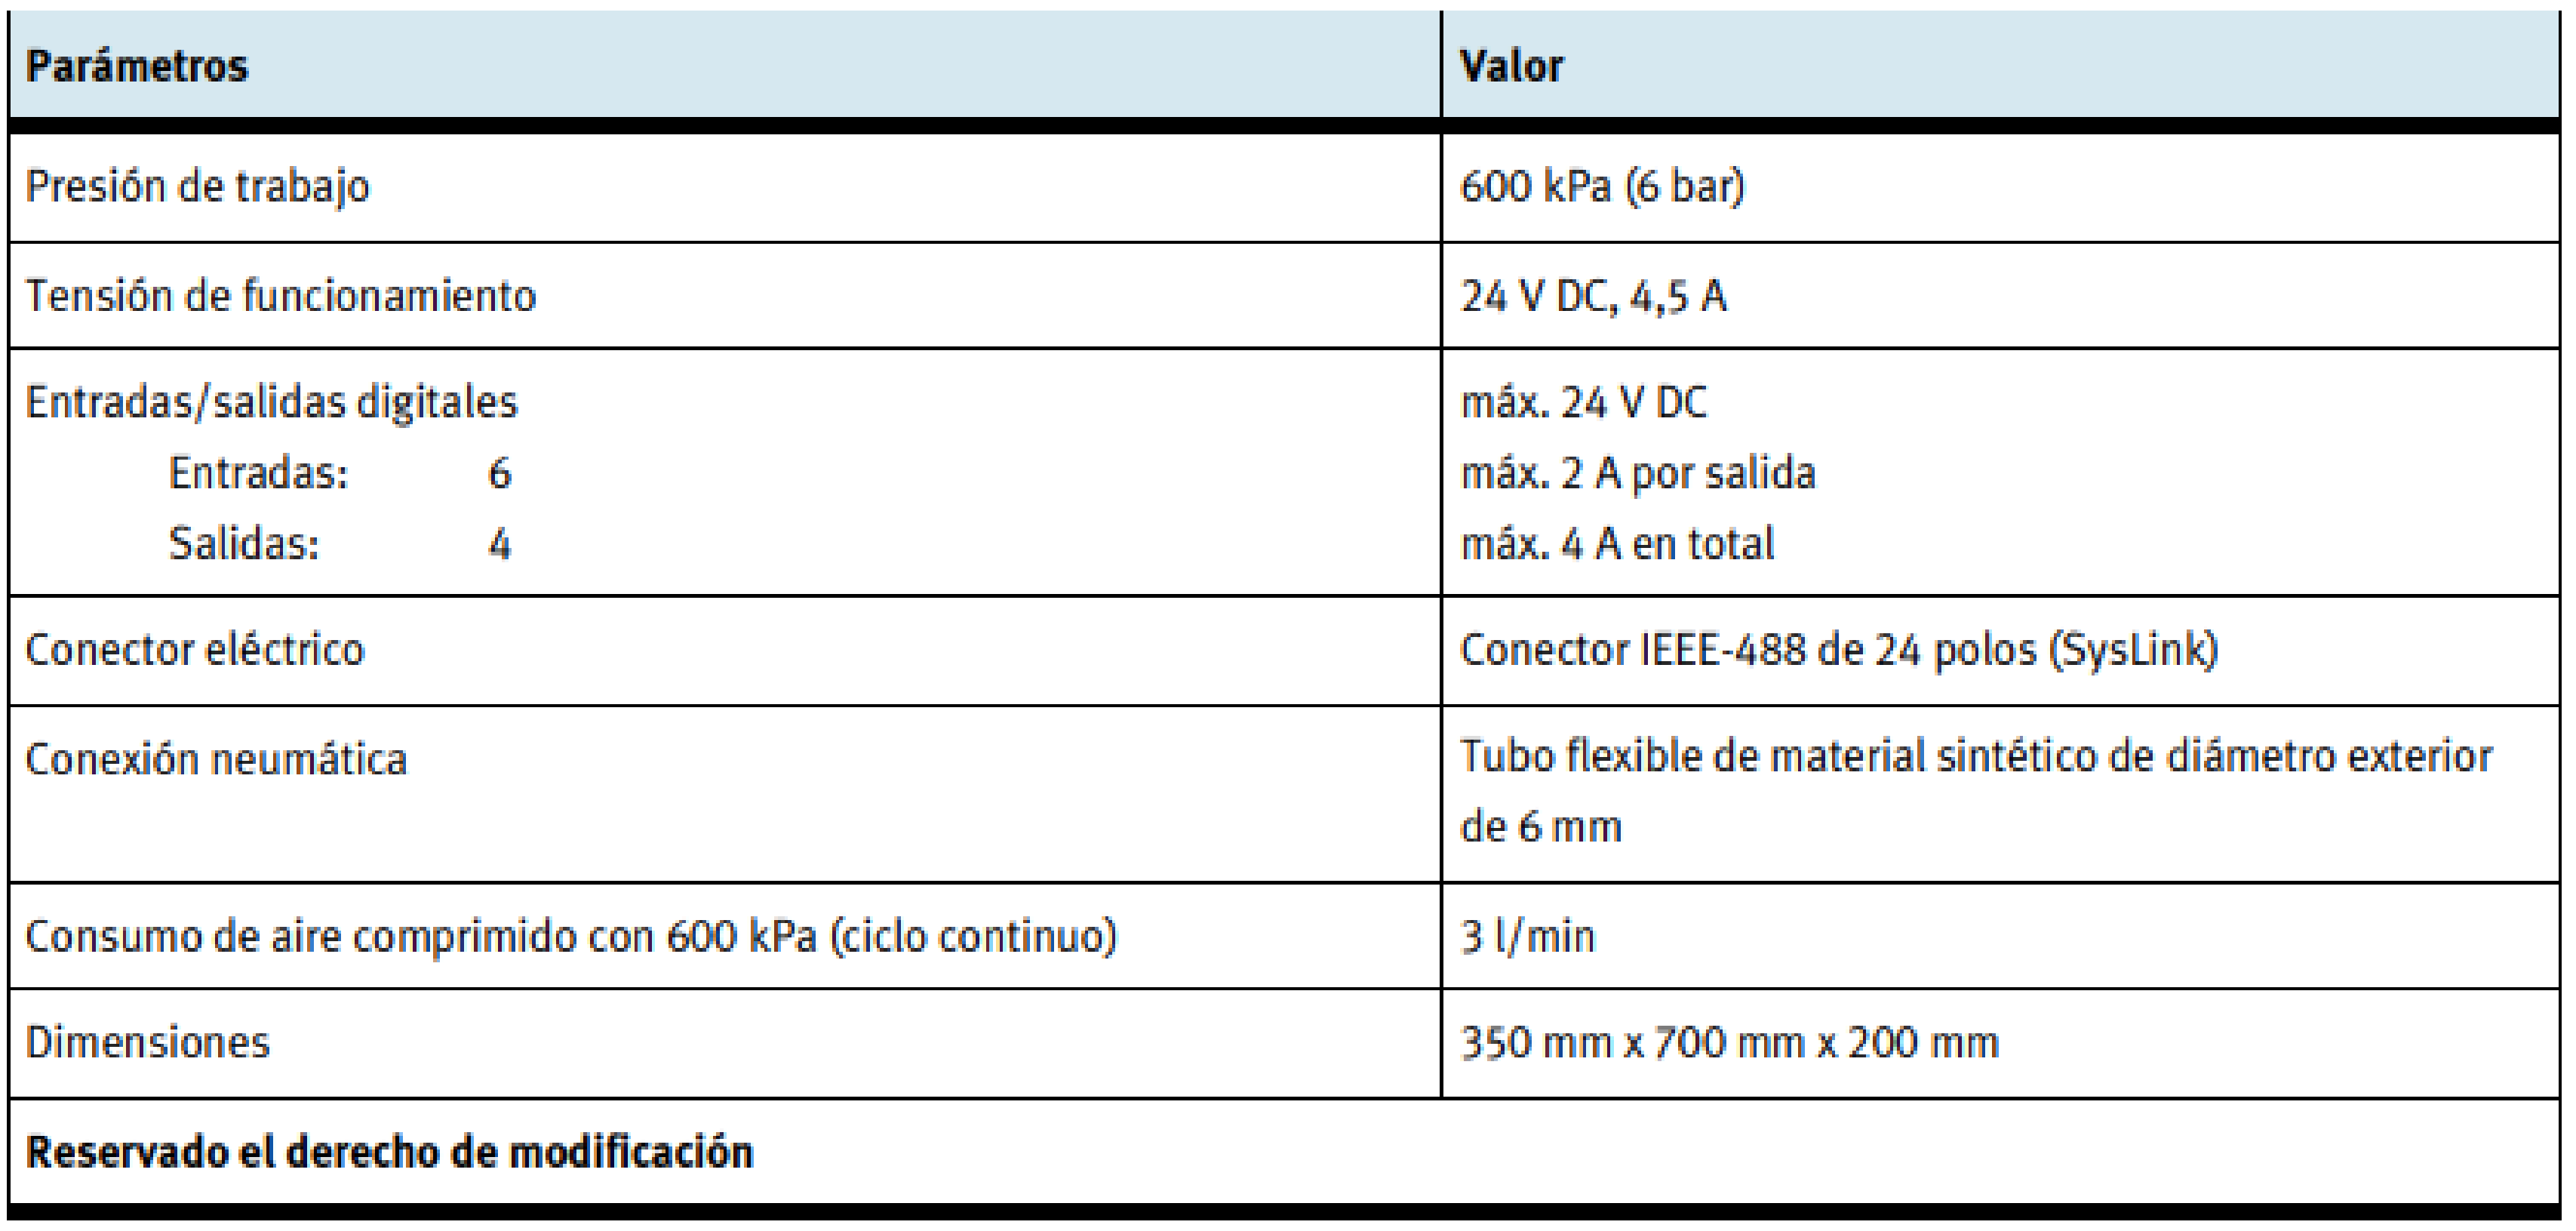
\includegraphics[width=15cm]{figs/estacion_distribucion_3}
  \end{center}
  \caption{\centering Características generales de la etación distribución. \cite{estacion_distribucion}}
  \label{fig:estacion_distribucion_3}
\end{figure} 

\clearpage

Las piezas utilizadas en las estaciones MPS de Festo Didactic suelen estar diseñadas en tres colores: rosa, negro y aluminio. Estas piezas representan distintos tipos de materiales o componentes y las diferencias de color permiten que los sensores ópticos las distingan fácilmente, lo que facilita su clasificación, inspección o tratamiento diferenciado por el sistema automatizado. Cada pieza mantiene dimensiones normalizadas para un manejo preciso y repetible y vienen equipadas con una tapa la cual puede ser colocada en estas para ofrecer mayor libertad al crear el proceso automático \\

La estación distribución está formada por los siguientes componentes:

\begin{itemize}
   \item \textbf{Stapelmagazin (almacén de piezas):} Sistema de alimentación que permite introducir piezas de trabajo de manera ordenada a mitad de la cinta transportadora. Funciona como un cargador vertical donde las piezas se apilan y se liberan una a una mediante un actuador neumático (máximo 7 piezas) \cite{estacion_distribucion}. Está diseñado para asegurar una alimentación controlada y repetible en los procesos de automatización \cite{estacion_distribucion}.
   
    \item \textbf{Cinta transportadora:} Encargada de desplazar las piezas entre las estaciones. Puede moverse en ambas direcciones. 
    
     \item \textbf{Separador:} Actuador neumático situada al inicio de la cinta cuya función es controlar el flujo de piezas en la cinta transportadora. Si se activa retiene las piezas provenientes del inicio de la cinta y da paso a las almacenadas en el almacén de piezas \cite{estacion_distribucion}.
     
      \item \textbf{Sensor para la distinción de piezas:} El sistema viene equipado con un módulo extra situado a la mitad de la cinta el cual es capaz de distinguir el color de la pieza. Si la pieza es de color negro se activa un bit, si es rosa se activan dos y si es metálica tres \cite{estacion_distribucion}.

    \item \textbf{Sensores:} La estación posee sensores ópticos y de proximidad que detectan la presencia, posición o características de las piezas, proporcionando datos al PLC.

    \item \textbf{Estructura mecánica modular:} Bastidor de perfiles de aluminio que soporta todos los componentes y permite su integración con otras estaciones del sistema MPS \cite{estacion_distribucion}.
\end{itemize}

\clearpage

\begin{figure} [h!]
  \begin{center}
    \includegraphics[width=17cm]{figs/estacion_distribucion_2}
  \end{center}
  \caption{\centering Componentes de la estación distribución.}
  \label{fig:estacion_distribucion_2}
\end{figure} 

\section{Estación unión}

La estación de unión de Festo Didactic\footnote{Image retrieved Festo.com.  (N.d.). Retrieved June 4, 2025, from  \url{https://www.festo.com/es/es/p/estacion-de-union-id_PROD_DID_8063910/}} simula un proceso industrial en el que se unen dos piezas mediante un actuador neumático equipado con una ventosa (Pick\&Place) \cite{estacion_union}. El objetivo de esta estación es colocerle o retirerle las tapas a las piezas que estén correctamente orientadas y así terminar la secuencia. La estación está compuesta por un brazo neumático, dos cintas para mover las piezas y tapas, sensores que detectan su presencia y adicionalmente un sensor cuya función es detectar la orientación de las piezas \cite{estacion_union}. Esta estación permite realizar prácticas de automatización como control secuencial, posicionamiento y verificación del montaje. Es ideal para formación técnica en tareas típicas de ensamblaje automatizadas. Además se adjuntan las características generales de la estación como se puede ver en el gráfico \ref{fig:estacion_union_3}:

\clearpage

\begin{figure} [h!]
  \begin{center}
    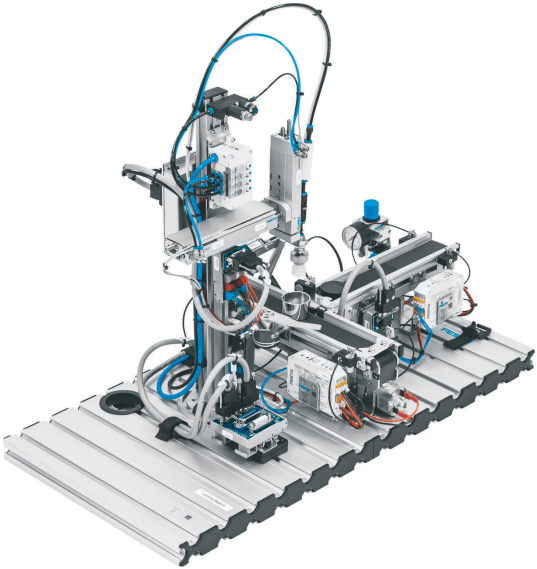
\includegraphics[width=10.75cm]{figs/estacion_union_1}
  \end{center}
  \caption{\centering Estación unión. \cite{estacion_union}}
  \label{fig:estacion_union_1}
\end{figure} 

\begin{figure} [h!]
  \begin{center}
    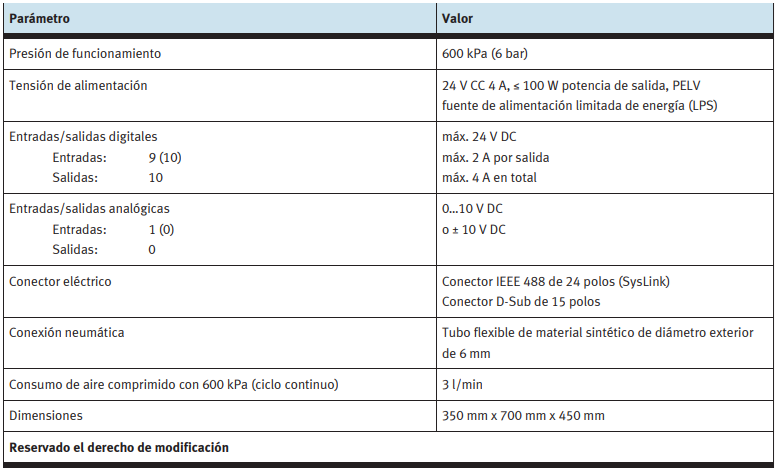
\includegraphics[width=15cm]{figs/estacion_union_3}
  \end{center}
  \caption{\centering Características generales de la estación unión. \cite{estacion_union}}
  \label{fig:estacion_union_3}
\end{figure} 

El Módulo de \textbf{Cinta Transportadora 1} transporta, separa y acumula piezas de hasta 40 mm de diámetro. Está impulsado por un motor de corriente continua con control de velocidad y dirección, y utiliza sensores ópticos para detectar la presencia de piezas al inicio, medio y al final de la cinta \cite{estacion_union}. Un electroimán que actúa como retenedor permite detener y liberar piezas individualmente a la altura del brazo, y un sensor difuso con salida digital y analógica identifica la orientación de las piezas el cual se ayuda de un retenedor para poder hacerlo correctamente sin que se mueva la pieza \cite{estacion_union}.

El Módulo de \textbf{Cinta Transportadora 2} tiene funciones similares, pero está diseñado para manejar tanto cuerpos de piezas como tapas. También utiliza un motor de corriente continua y sensores ópticos para controlar el flujo de materiales \cite{estacion_union}.

El Módulo \textbf{Pick\&Place} es un manipulador de dos ejes que utiliza carros deslizantes de precisión y sensores de proximidad para detectar las posiciones finales. Puede equiparse con una ventosa de fuelle o un gripper paralelo para agarrar las piezas, y cuenta con un filtro de vacío y un presostato para asegurar una sujeción fiable \cite{estacion_union}. La fuerza del eje vertical puede ajustarse mediante un regulador de presión, y el módulo incluye todos los componentes necesarios para su funcionamiento, como generador de vacío, válvulas y conexiones eléctricas \cite{estacion_union}.

\begin{figure} [h!]
  \begin{center}
    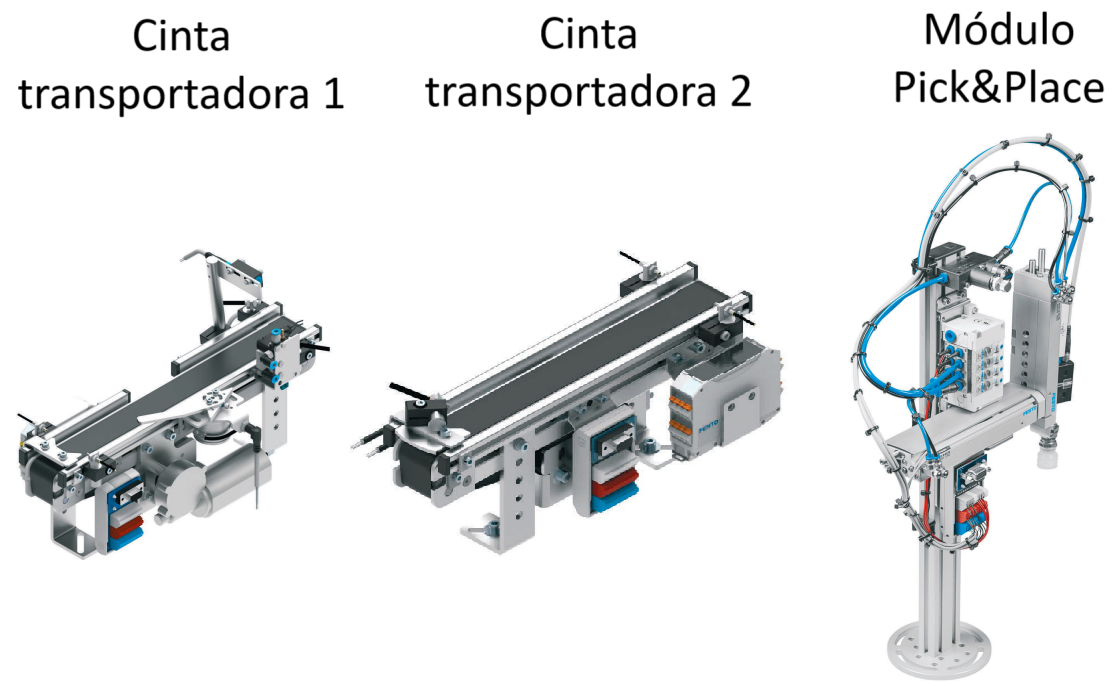
\includegraphics[width=14.5cm]{figs/estacion_union_2}
  \end{center}
  \caption{\centering Componentes de la estación unión. \cite{estacion_union}}
  \label{fig:estacion_union_2}
\end{figure} 

\begin{figure} [h!]
  \begin{center}
    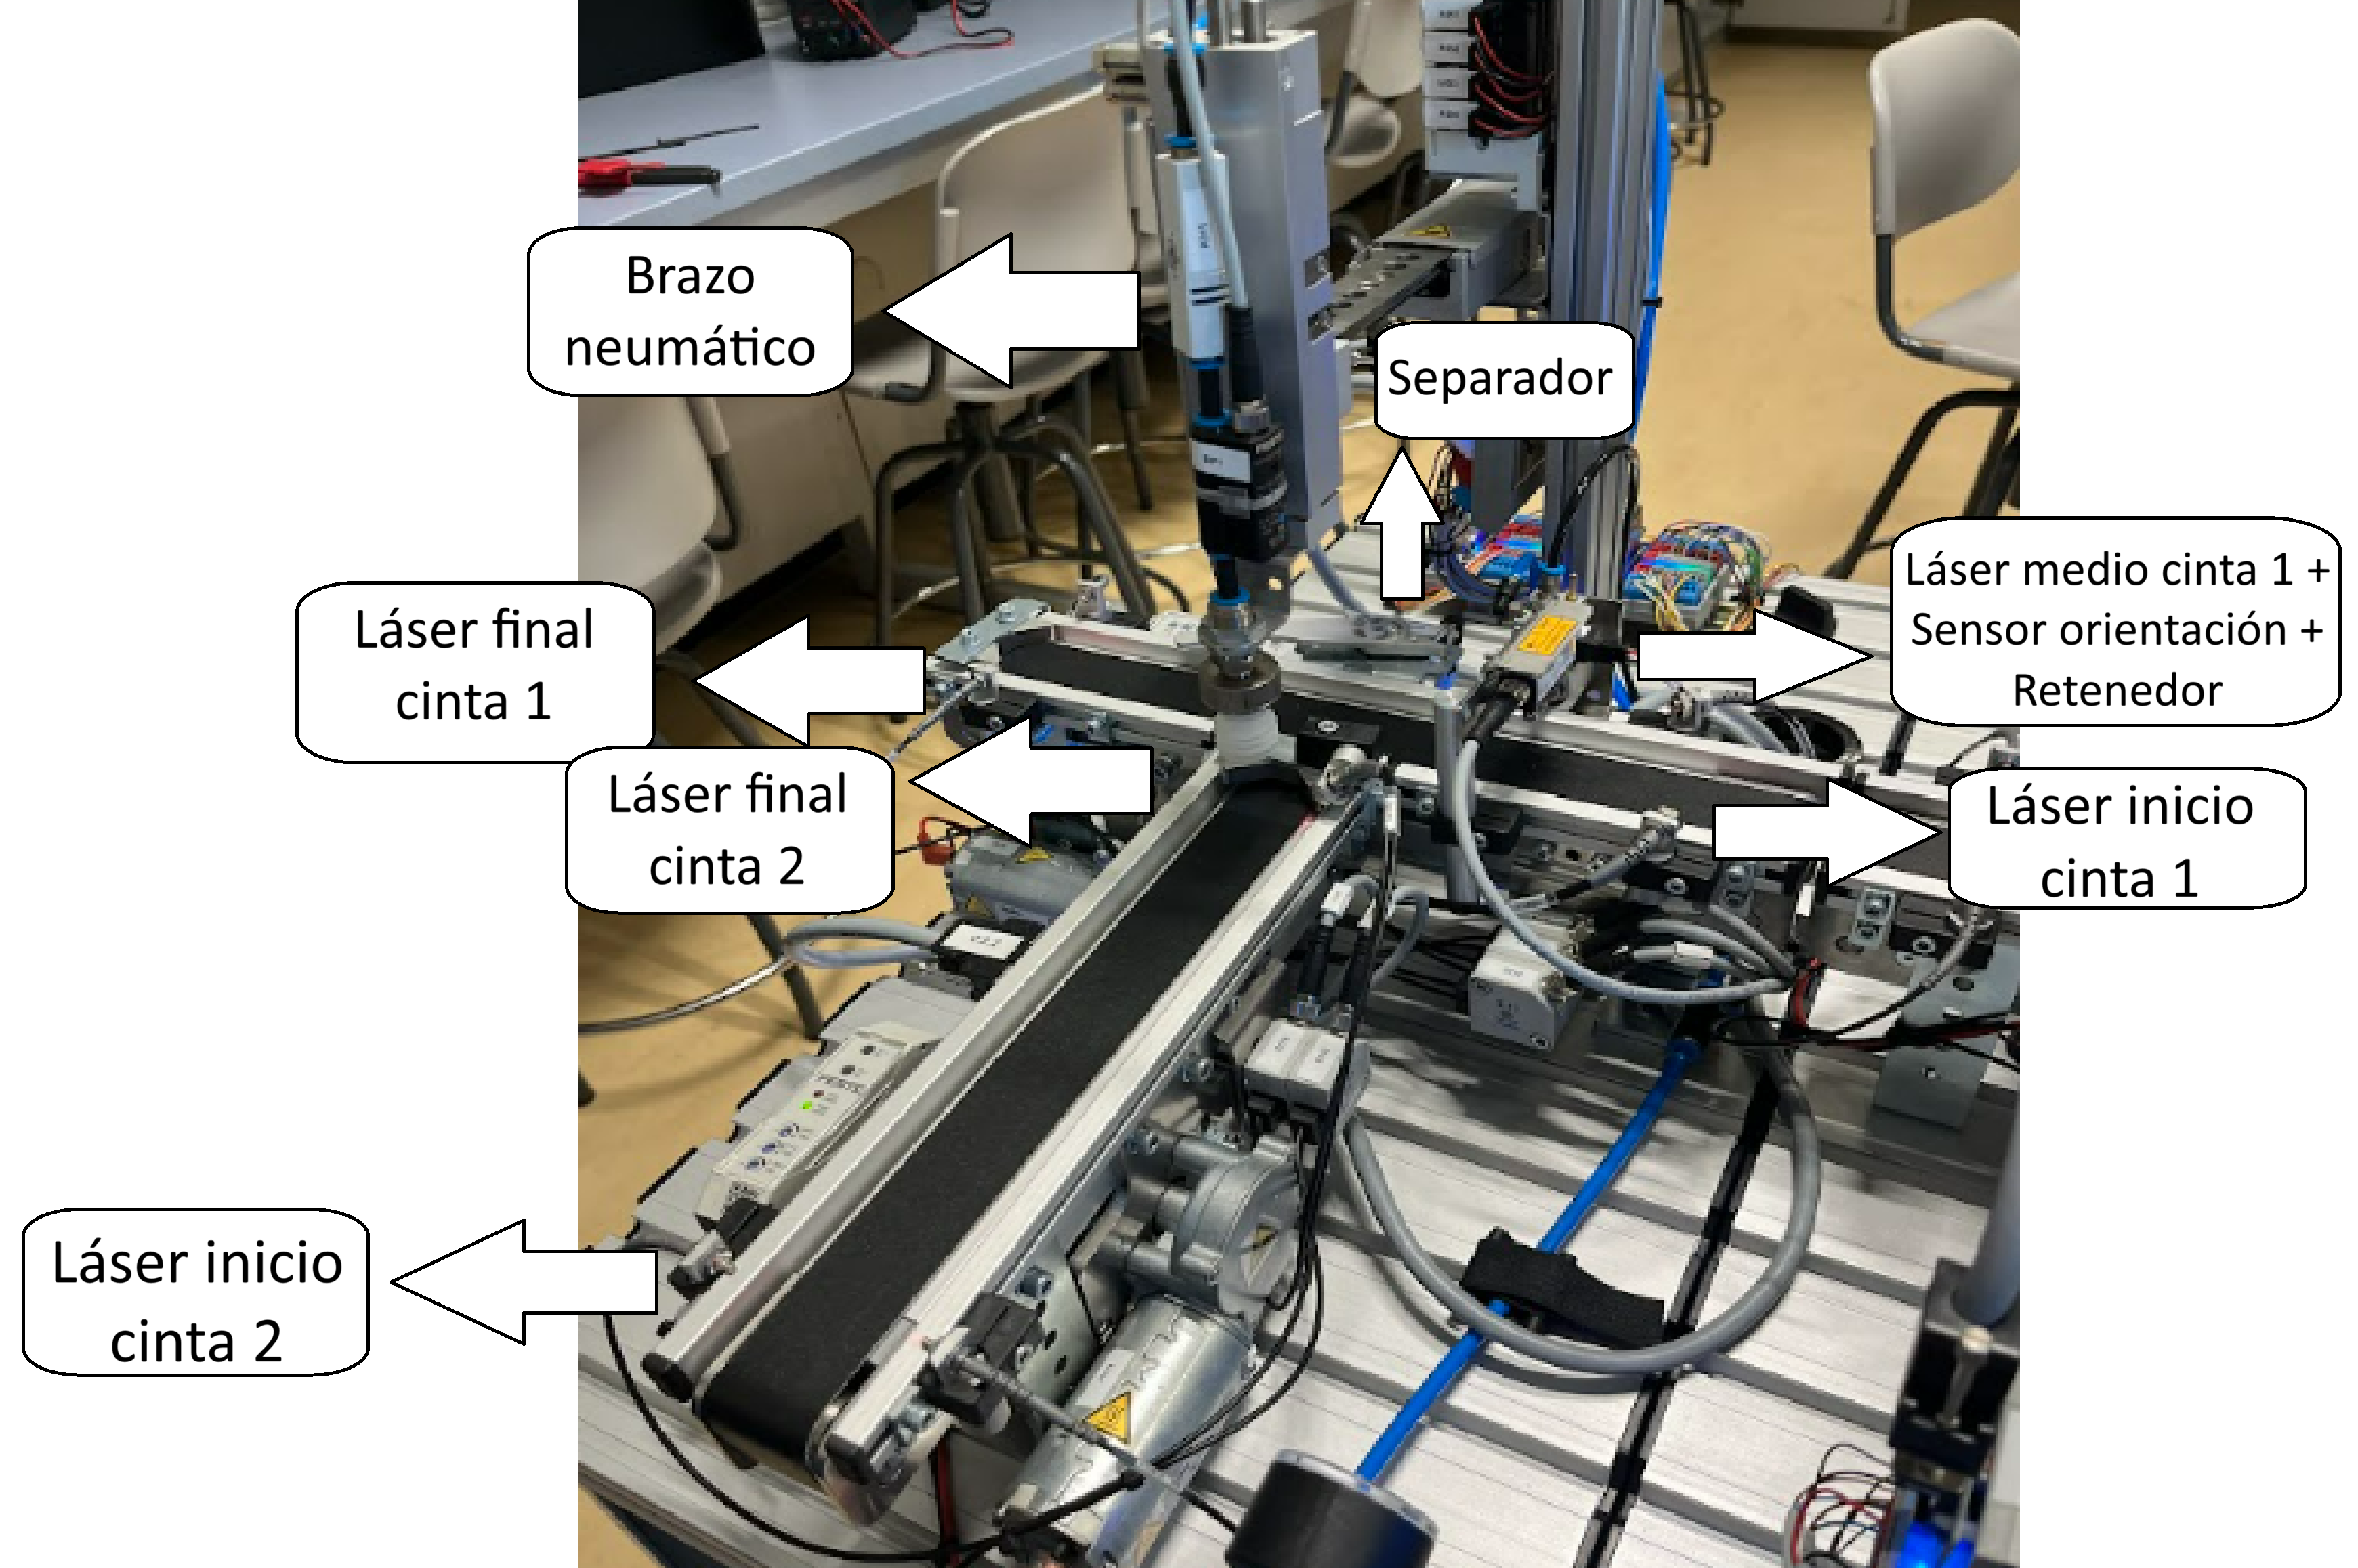
\includegraphics[width=16.5cm]{figs/estacion_union_4}
  \end{center}
  \caption{\centering Componentes de la estación unión.}
  \label{fig:estacion_union_4}
\end{figure} 

\section{PLCs Siemens 1200s}

Para la elaboración de este trabajo se ha utilizado el PLC Siemens S7-1200, concretamente el modelo \textbf{6ES7 215-1BG40-0XB0}. Este modelo forma parte de la familia de controladores compactos de Siemens, ampliamente utilizados en aplicaciones de automatización industrial. El PLC corresponde a la CPU 1215C con alimentación AC/DC y salidas a relé, lo que le otorga una gran versatilidad para controlar y supervisar sistemas de pequeña y mediana escala \cite{PLC_siemens}.

Entre sus características más destacadas se encuentran sus 14 entradas digitales de 24 V DC, 10 salidas digitales tipo relé de 2 A, 2 entradas analógicas (0–10 V DC) y 2 salidas analógicas (0–20 mA DC) \cite{PLC_siemens}. Esta combinación de entradas y salidas permite conectar una gran variedad de sensores y actuadores directamente al PLC sin necesidad de módulos adicionales, lo que reduce costes y espacio en armarios de control.

En términos de comunicación, esta CPU incorpora dos puertos PROFINET con función de switch integrado, lo que facilita su integración en redes industriales y la comunicación con dispositivos HMI, otros PLCs o sistemas SCADA \cite{PLC_siemens}. Además, es compatible con protocolos de comunicación abiertos como TCP/IP, ISO-on-TCP, UDP y MODBUS, y permite el uso de servidor OPC UA mediante licencia, una característica clave para entornos de Industria 4.0 \cite{PLC_siemens}.

\begin{figure} [h!]
  \begin{center}
    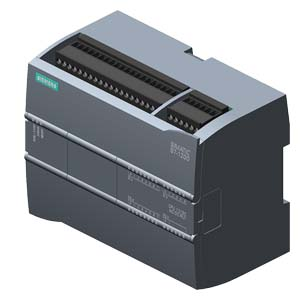
\includegraphics[width=8cm]{figs/PLC_siemens}
  \end{center}
  \caption{\centering PLC Siemens 1215 AC/DC/RLY. \cite{PLC_siemens}}
  \label{fig:PLC_siemens}
\end{figure} 

Su programación se realiza a través del software \textbf{STEP 7 (TIA Portal)} versión V20 o superior, ofreciendo compatibilidad con lenguajes como KOP (diagrama de contactos), FUP (diagrama de funciones) y SCL (lenguaje estructurado) \cite{PLC_siemens}. También dispone de funciones tecnológicas avanzadas como control PID, contadores de alta velocidad (hasta 100 kHz), y posicionamiento, lo cual amplía sus capacidades para aplicaciones más exigentes \cite{PLC_siemens}.

En cuanto a su hardware, presenta una memoria de trabajo de 200 kB y una memoria de carga de 4 MB, además de la posibilidad de insertar una tarjeta SIMATIC Memory Card para ampliar almacenamiento o realizar copias de seguridad \cite{PLC_siemens}. El diseño compacto (130 × 100 × 75 mm) y el grado de protección IP20 lo hacen ideal para entornos industriales controlados.

\section{HMI}

El HMI utilizado para este proyecto es el \textbf{SIMATIC HMI KTP700 Basic PN}. Este es un panel HMI de la segunda generación de Basic Panels de Siemens, diseñado para ofrecer una interfaz hombre-máquina eficiente, compacta y rentable en tareas de visualización y operación dentro de entornos industriales. Este modelo cuenta con una pantalla táctil de 7 pulgadas, con una resolución de 800 × 480 píxeles (WVGA) y una profundidad de color de 64.000 colores, lo que proporciona una visualización clara, detallada y moderna de los procesos industriales \cite{HMI_KTP}.

Una de sus principales ventajas es la combinación de pantalla táctil y teclas de función (8 teclas de función programables), lo cual permite al operador interactuar de forma rápida e intuitiva con el sistema, incluso con guantes o en entornos con condiciones difíciles. El panel también está equipado con una interfaz PROFINET integrada, lo que lo hace ideal para la comunicación directa con controladores SIMATIC S7-1200 y otros dispositivos de automatización compatibles \cite{HMI_KTP}.

\begin{figure} [h!]
  \begin{center}
    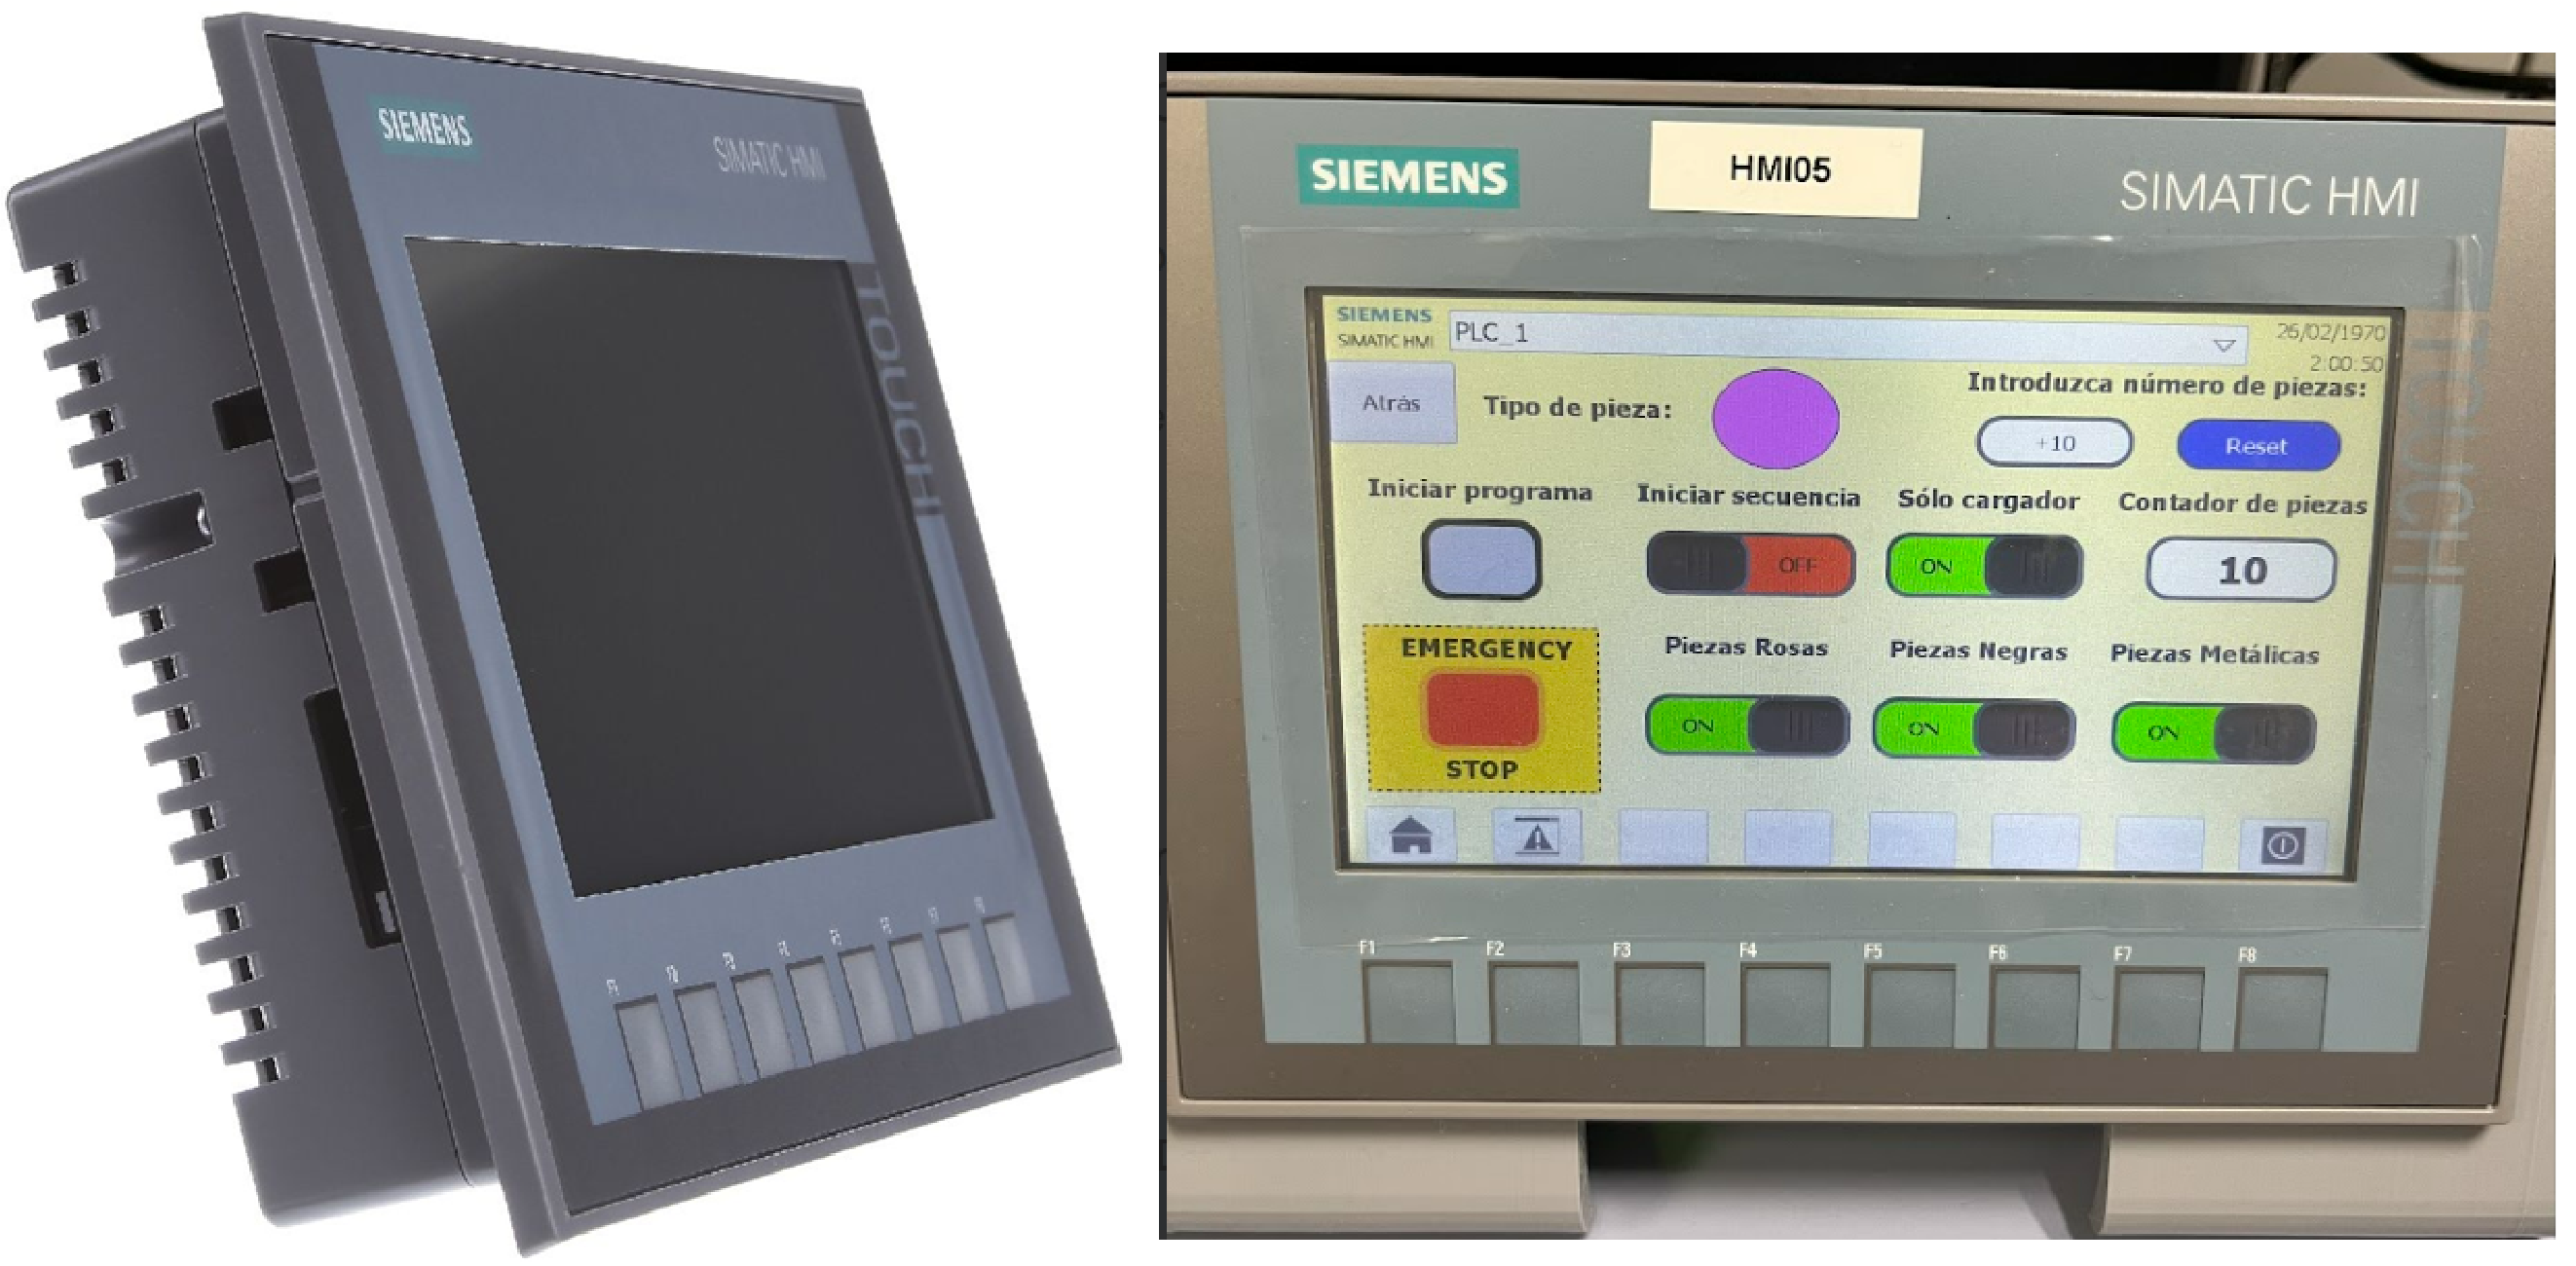
\includegraphics[width=15cm]{figs/HMI_cap_3}
  \end{center}
  \caption{\centering SIMATIC HMI KTP700 Basic PN.}
  \label{fig:HMI_cap_3}
\end{figure} 

El KTP700 Basic PN dispone de una interfaz USB que permite conectar dispositivos periféricos como ratones, teclados o memorias USB para la transferencia de recetas, actualizaciones de firmware o copias de seguridad de datos de usuario \cite{HMI_KTP}. Además, este HMI admite la configuración y programación a través del entorno de desarrollo TIA Portal (Totally Integrated Automation) con WinCC Basic, lo que asegura una integración coherente y eficiente con el resto de componentes del sistema de automatización \cite{HMI_KTP}.

En cuanto a su diseño físico, el dispositivo tiene unas dimensiones compactas de 214 × 158 × 39 mm y está pensado para montaje en panel \cite{HMI_KTP}. Cuenta con una protección frontal IP65, lo que le confiere resistencia frente a polvo y chorros de agua, haciéndolo apto para condiciones industriales exigentes \cite{HMI_KTP}. También incluye funciones como alarmas, tendencias, gestión de recetas y multilenguaje, lo que lo convierte en una solución versátil para aplicaciones industriales básicas.

\section{TIA Portal}

TIA Portal (Totally Integrated Automation Portal) es una plataforma de ingeniería desarrollada por Siemens que integra en un único entorno todas las herramientas necesarias para la configuración, programación, supervisión y mantenimiento de sistemas de automatización industrial. Fue diseñado con el objetivo de unificar y simplificar la ingeniería de proyectos, mejorando la eficiencia en el desarrollo, la puesta en marcha y la operación de sistemas de control.

\begin{figure} [h!]
  \begin{center}
    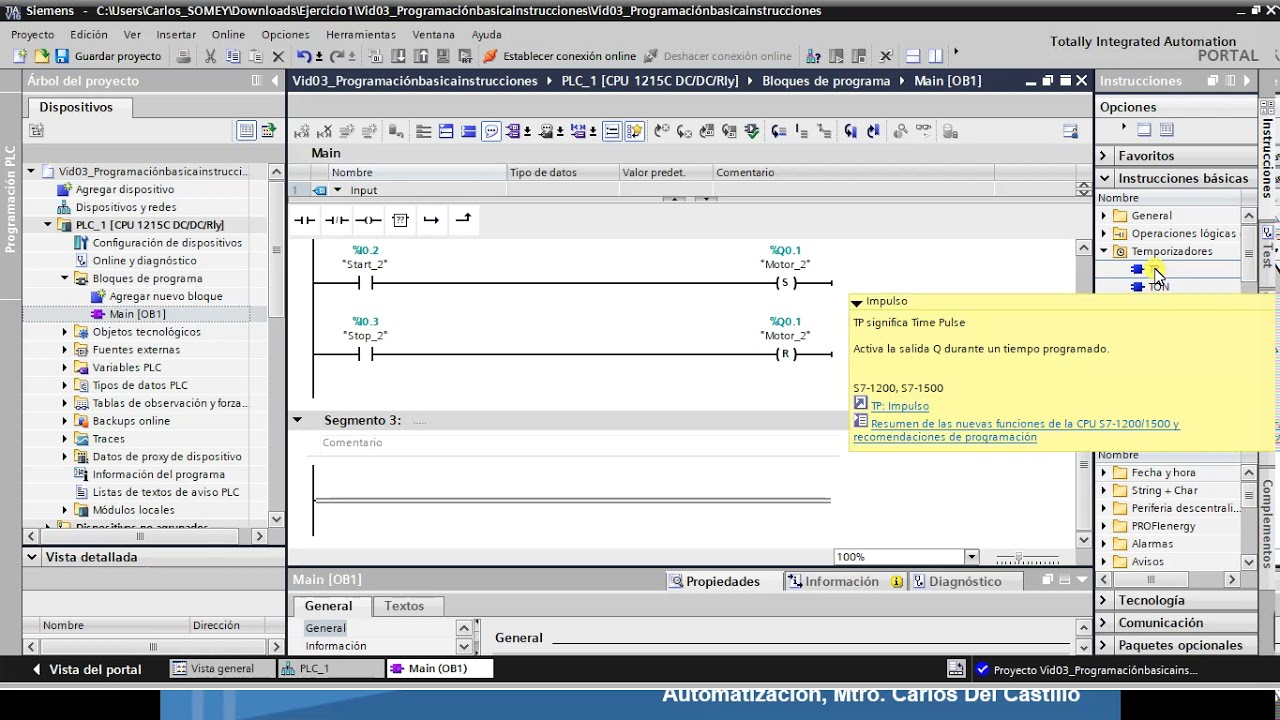
\includegraphics[width=14cm]{figs/TIA_portal}
  \end{center}
  \caption{\centering Pantallazo de la aplicación TIA Portal.}
  \label{fig:TIA_portal}
\end{figure} 

Esta plataforma permite trabajar de forma integrada con controladores PLC, interfaces HMI, sistemas SCADA, variadores de velocidad, dispositivos de seguridad y redes industriales, todo desde una única interfaz \cite{TIA_portal}. El entorno TIA Portal combina software como STEP 7 (para programación de PLC), WinCC (para interfaces HMI y SCADA), Startdrive (para variadores SINAMICS), Safety Advanced (para funciones de seguridad) y Energy Suite (para gestión energética) \cite{TIA_portal}.

En este proyecto se ha utilizado la versión \textbf{TIA Portal V16}, la cual permitedividir los proyectos en unidades de software independientes, permitiendo una programación modular con interfaces definidas \cite{TIA_portal}. Esto facilita la colaboración entre varios ingenieros, mejora la reutilización de código y simplifica la gestión de proyectos complejos.

En cuanto a la programación de PLCs, TIA Portal V16 ofrece soporte completo para los controladores SIMATIC S7-1200, S7-1500, S7-300 y S7-400, así como para soluciones de seguridad integradas mediante STEP 7 Safety \cite{TIA_portal}. La integración con WinCC permite el diseño y configuración de interfaces HMI.

La plataforma también incluye herramientas de simulación como PLCSIM y HMISIM, que permiten probar y validar la lógica de control y las interfaces HMI sin necesidad de hardware físico \cite{TIA_portal}. Esto reduce los tiempos de desarrollo y facilita la detección temprana de errores. Además, la compatibilidad con estándares abiertos y protocolos de comunicación como PROFINET, OPC UA y Modbus garantiza una integración fluida con otros sistemas y dispositivos en entornos de automatización industrial \cite{TIA_portal}.

\section{Brazo UR5e}

El UR5e es un brazo robótico colaborativo de seis ejes desarrollado por Universal Robots, diseñado para automatizar tareas industriales de forma segura y eficiente. Con una capacidad de carga útil de hasta 5 kg y un alcance de 850 mm, el UR5e es especialmente adecuado para aplicaciones que requieren precisión y flexibilidad, como ensamblaje, manipulación de materiales, soldadura ligera y pruebas de calidad \cite{UR5e}.

\begin{figure} [h!]
  \begin{center}
    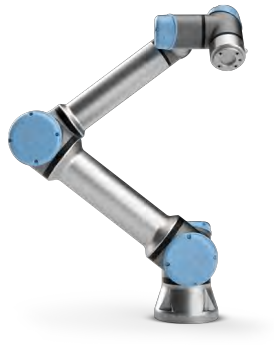
\includegraphics[width=8.4cm]{figs/UR5e}
  \end{center}
  \caption{\centering Robot UR5e de Universal Robots. \cite{UR5e}}
  \label{fig:UR5e}
\end{figure} 

Una de las características distintivas del UR5e es su diseño colaborativo, que permite su integración en entornos donde comparte espacio con operadores humanos sin necesidad de barreras de seguridad, siempre que se realice una evaluación de riesgos adecuada \cite{UR5e}. Esto es posible gracias a sus sensores de fuerza y par integrados, que detectan contactos inesperados y detienen el movimiento del robot para evitar lesiones o daños \cite{UR5e}.

El UR5e se controla mediante el software PolyScope, una interfaz intuitiva que se opera a través de un panel de enseñanza con pantalla táctil. PolyScope permite programar el robot de manera sencilla, incluso sin experiencia previa en programación, mediante la guía manual del brazo para enseñar posiciones y trayectorias \cite{UR5e}. Para usuarios avanzados, también se ofrece la posibilidad de programar utilizando el lenguaje URScript, lo que proporciona un mayor control y flexibilidad en aplicaciones complejas.

Su diseño ligero, con un peso total de aproximadamente 20,6 kg, permite montarlo en diversas orientaciones y ubicaciones, adaptándose a diferentes necesidades de producción \cite{UR5e}. Además, el UR5e es compatible con una amplia gama de accesorios y herramientas a través del ecosistema UR+, que ofrece soluciones certificadas para tareas específicas, como pinzas, cámaras y sensores adicionales \cite{UR5e}. 

\begin{figure} [h!]
  \begin{center}
    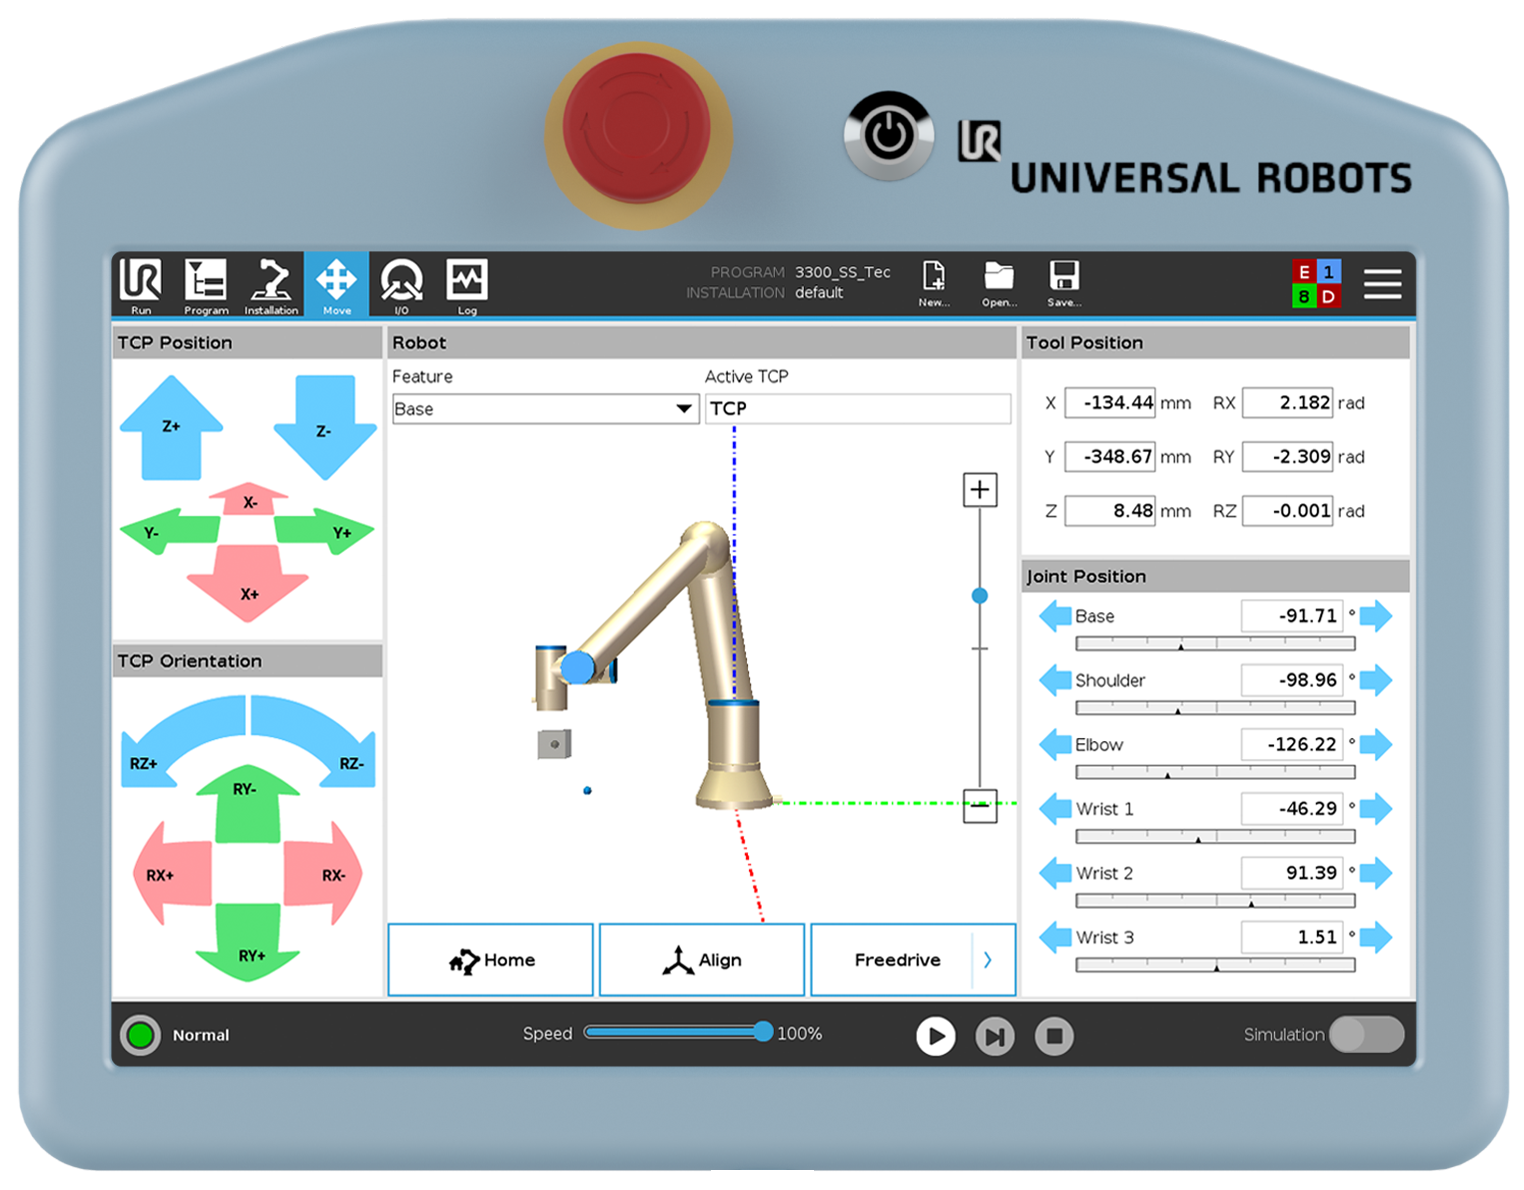
\includegraphics[width=10.5cm]{figs/PolyScope}
  \end{center}
  \caption{\centering Pantalla táctil PolyScope. \cite{PolyScope_img}}
  \label{fig:PolyScope}
\end{figure} 




\chapter{Diseño}
\label{cap:capitulo4}

\begin{flushright}
\begin{minipage}[]{10cm}
\emph{En la industria, la precisión no es un lujo: es la esencia de la automatización.}\\
\end{minipage}\\

Anónimo \\
\end{flushright}

\vspace{1cm}

En este capítulo se abarca y explica el diseño completo del sistema automatizado desarrollado. En él se describen tanto los aspectos físicos de la instalación como la lógica de control implementada, abordando la selección de componentes, la configuración de la red de comunicación, y el funcionamiento de cada estación: distribución, unión y brazo robótico colaborativo. Se explican las conexiones entre los dispositivos, incluyendo los sensores, actuadores, PLCs, la interfaz HMI y el UR, así como la implementación de los distintos modos de operación mediante la Guía GEMMA, que ha servido de base para estructurar el comportamiento del sistema. Para terminar se hará un pequeño resumen del resultado final obtenido como consecuencia del trabajo realizado.

\section{Descripción general}
\label{sec:descripcion_general}

El objetivo de este trabajo es lograr que el ciclo de producción comience en la estación de distribución, donde se filtra el tipo y número de piezas que se quieren producir, después pasan a la estación unión donde se le colocará una tapa encima de las piezas bien orientadas, y finalmente, el brazo UR cogerá la pieza y la colocará en un palé para su posterior almacenamiento. 

En la sección \ref{sec:descripcion} ya se presentó una visión general del objetivo del proyecto, pero en esta se profundizará en él con una descripción más detallada y específica. El sistema global está compuesto por dos PLCs, una interfaz HMI y un robot colaborativo UR5e. Una parte fundamental del trabajo es garantizar una comunicación fluida y fiable entre todos los componentes para asegurar un funcionamiento coordinado y realista. El trabajo va a ser desarrollado en TIA portal y la comunicación via PROFINET. \\

El objetivo final es desarrollar un ciclo de producción en el que intervengan todos los componentes mencionados, simulando una aplicación industrial realista. Para ello, el ciclo debe iniciarse en la estación de distribución, donde se introducen las piezas en el proceso productivo y se identifica el tipo de material que las compone, con el fin de determinar el tratamiento correspondiente en función de sus características. Los parámetros de distinción de piezas se establecen en el HMI por el operario, si se descarta la pieza, se acabará el ciclo y se empezará de nuevo, pero si es aceptada pasará a la estación unión continuando el proceso. 

Para que la estación unión comience su proceso dentro del ciclo, es necesario que el PLC que controla la estación distribución le envíe un mensaje al segundo PLC (el que controla la estación unión) para informarle de que debe empezar.  Una vez recibido el mensaje, la segunda estación inicia el proceso tomando la pieza y deteniéndola para verificar su orientación. Si la orientación es correcta, la pieza continúa su avance en el ciclo; en caso contrario, se genera un mensaje de error en el HMI y la pieza es descartada, regresando a la estación de distribución, donde se requerirá una nueva comunicación para reiniciar el proceso. Si la pieza está bien orientada continuará su camino hasta que se pare en un punto donde la tapa proveniente de otra cinta será colocada encima de la pieza con el módulo pick \& place. Una vez terminado el ciclo la estación volverá a comunicarse con la estación unión para hacerle saber que terminó su proceso.

Una vez que el PLC de la estación unión recive el mensaje de fin de ciclo del otro PLC, el último paso es comunicarse con el UR para que termine el proceso global. El PLC asociado a la estación distribución es el encargado de mandar el mensaje vía Profinet al UR, quién iniciará una secuencia de paletizado simulando la ordenación de las piezas. Como físicamente las estaciones Festo y el UR están separadas, el proceso de paletizado del brazo robótico se realiza con bricks de leche como elemento manipulable. En el momento que el UR termine su proceso, el PLC será notificado terminando con el ciclo global y volviendo a empezar.

La función del HMI en este proyecto será proporcionar al operario una representación simplificada del sistema, permitiéndole controlarlo mediante unos pocos botones. A través de la pantalla se gestionan funciones como el inicio y la parada del sistema, la configuración del número de piezas a procesar y la selección del tipo de material permitido. Además, el HMI se utiliza para mostrar mensajes de error, como la detección de una pieza mal orientada o la notificación de que el robot UR está colocando una pieza en el palé.

\clearpage

\begin{figure}[h!]
  \begin{center}
    \includegraphics[width=13cm]{figs/sistemas_unidos}
  \end{center}
  \caption{\centering Estación distribución y estación unión unidas.}
  \label{fig:sistemas_unidos}
\end{figure}


\section{Conectividad de los dispositivos}
\label{sec:conectividad_dispositivos}

Para realizar la conexión de todos los dispositivos entre si, se ha utilizado el switch Ethernet industrial SCALANCE XB005 y el protocolo PROFINET, los cuales ya se ha explicado en el capítulo \ref{cap:capitulo3}. Este dispositivo cuenta con 5 puertos, soporta conexiones PROFINET y está pensado para usarse en fábricas o instalaciones automatizadas donde se requiere una red estable y confiable. El switch es ideal para el proyecto ya que se necesita comunicar 4 dispositivos más el ordenador que los programa entre ellos, ocupando los 5 puertos disponibles. Los cables Ethernet utilizados en son el modelo 6XV18703QN10 \footnote{6XV18703QN10. (n.d.). Radwell.eu. Retrieved June 10, 2025, from \url{https://www.radwell.eu/es/buy/siemens-6xv18703qn10/1018547.html}} los cuales están especialmente diseñados para este tipo de aplicaciones industriales.  \\

A continuación, se muestra un diagrama de conexiones de todos los dispositivos:

\begin{figure} [h!]
  \begin{center}
    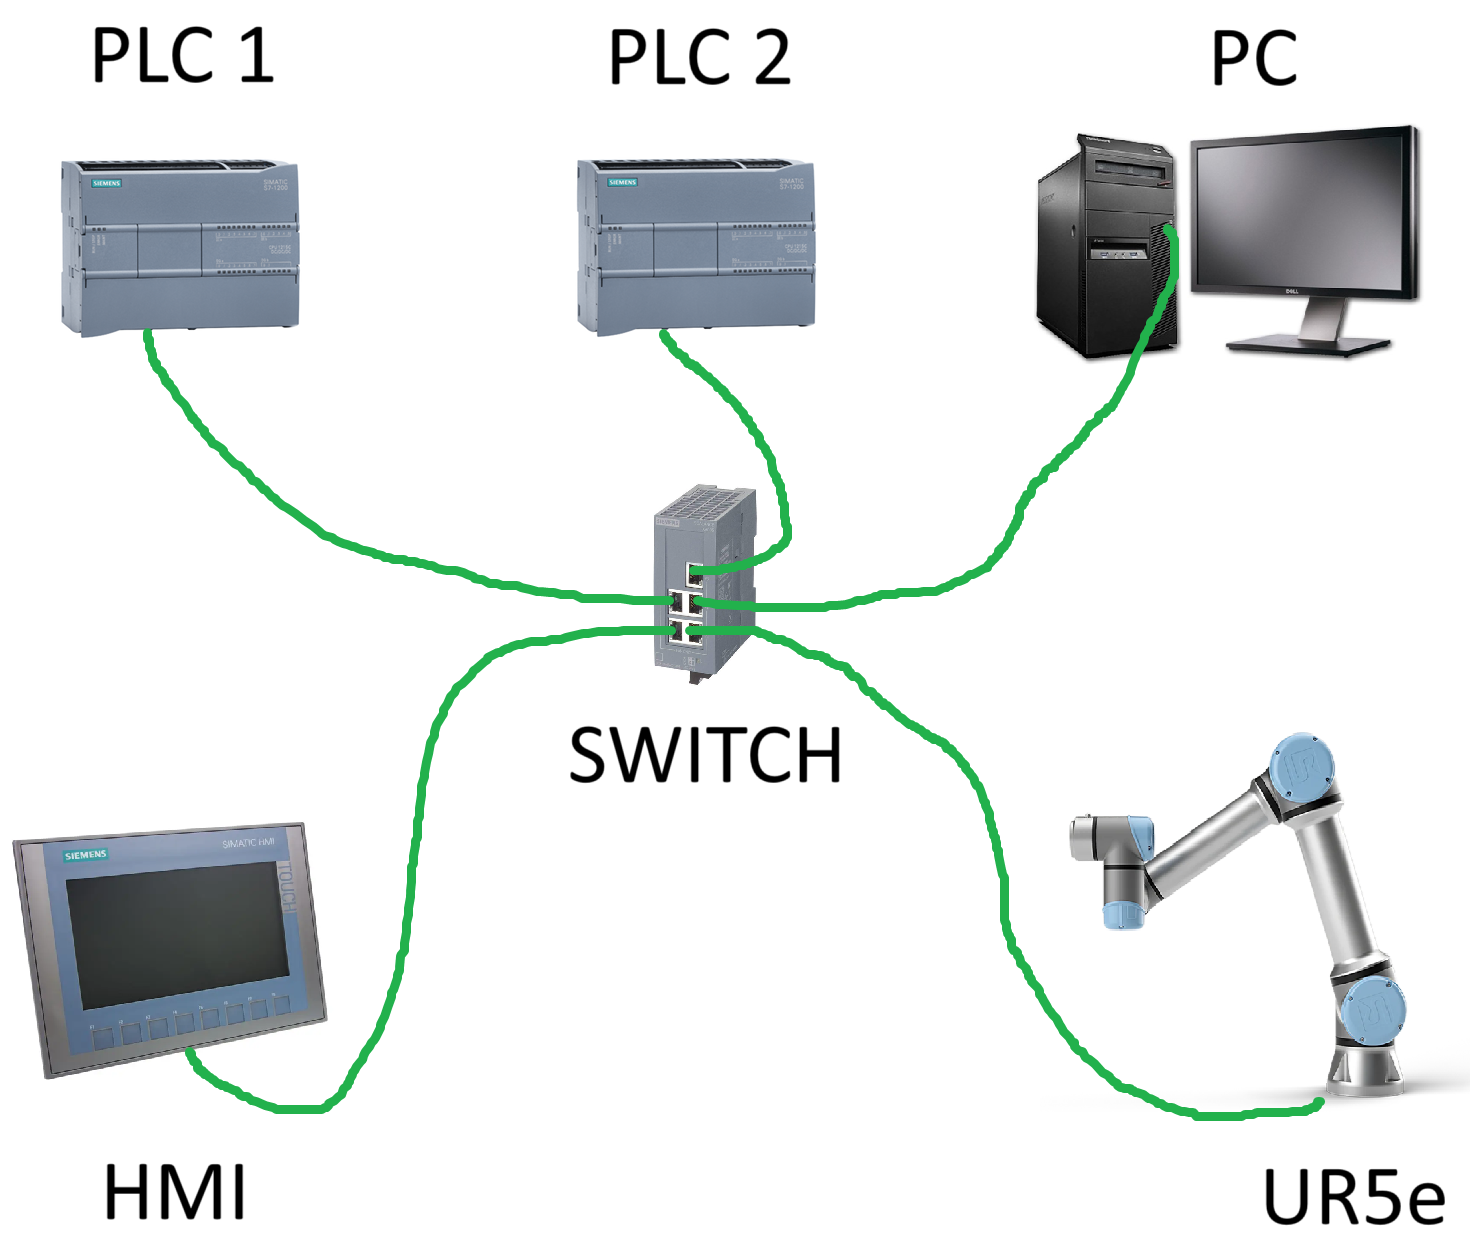
\includegraphics[width=14cm]{figs/conexion_dispositivos}
  \end{center}
  \caption{\centering Representación de conexiones entre los dispositivos del proyecto.}
  \label{fig:conexion_dispositivos}
\end{figure} 

\begin{figure} [h!]
  \begin{center}
    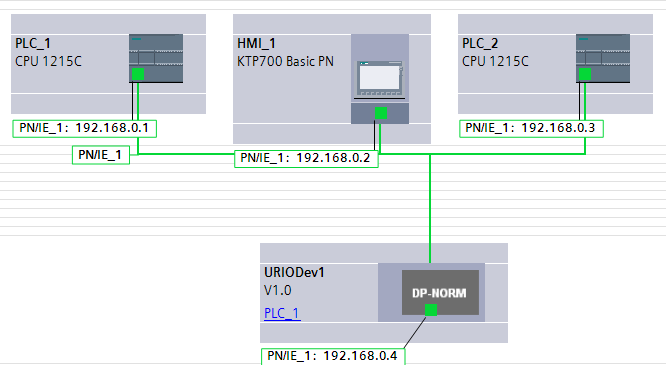
\includegraphics[width=15cm]{figs/conexiones_tiaportal}
  \end{center}
  \caption{\centering Representación de conexiones entre los dispositivos dentro del proyecto de Tia Portal.}
  \label{fig:conexiones_tiaportal}
\end{figure} 

\clearpage

Para intercambiar mensajes y datos entre los dos PLCs se han utilizado las funciones de comunicación RECV y SEND. SEND permite enviar información desde un PLC a otro, mientras que RECV se encarga de recibir esos datos en el destino. Estas funciones son muy útiles para coordinar procesos distribuidos y compartir datos en tiempo real en redes como Ethernet/IP o Profinet. Para la comunicación entre los PLCs, se ha definido una estructura de datos específica para cada uno, la cual se utiliza en el intercambio de mensajes. Las estructuras mostradas en la imagen \ref{fig:estructura_com_plcs} incluyen variables booleanas utilizadas para la comunicación de tres posibles finalizaciones de ciclo, así como una variable entera que indica el tipo de pieza detectada. Contienen toda la información necesaria para el proceso, permitiendo compartir y sincronizar los datos de forma eficiente entre los distintos controladores. Cada PLC envía y recibe mensajes a una frecuencia de 5Hz y van activando o desactivando los campos de la estructura según en la etapa que se encuentren. Seguidamente se muestra una imagen de las estructuras de datos y las funciones de comunicación de los PLCs: \\

\begin{figure} [h!]
  \begin{center}
    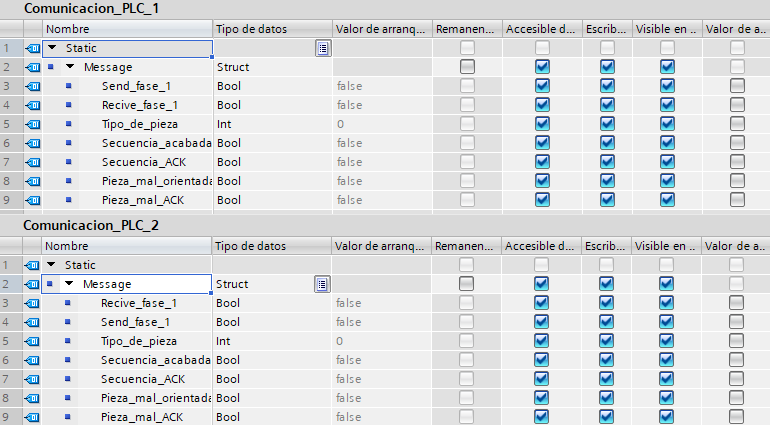
\includegraphics[width=16cm]{figs/estructura_com_plcs}
  \end{center}
  \caption{\centering Estructuras de datos utilizadas en la comunicación entre los PLCs.}
  \label{fig:estructura_com_plcs}
\end{figure} 

\clearpage

\begin{figure} [h!]
  \begin{center}
    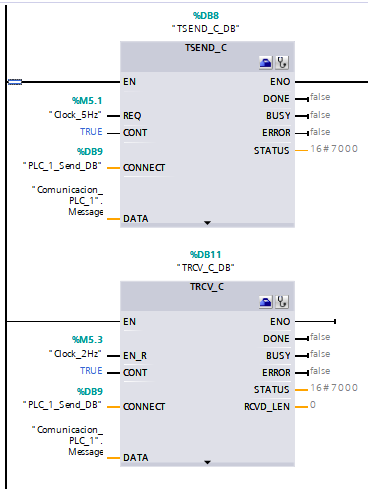
\includegraphics[width=10cm]{figs/comunicacion_plcs}
  \end{center}
  \caption{\centering Funciones SEND y RECV entre los PLCs.}
  \label{fig:comunicacion_plcs}
\end{figure} 

Para establecer la comunicación entre el UR y el PLC (el conectado a la estación distribución) a través de PROFINET, se ha seguido la guía oficial de UR PROFINET\footnote{Profinet Guide - 20596. (n.d.). Universal-robots.com. Retrieved June 25, 2025, from \url{https://www.universal-robots.com/articles/ur/interface-communication/profinet-how-to-guide-e-series/}}. El primer paso es activar la funcionalidad PROFINET en el UR, accediendo a la pestaña “Instalación” de este, esta acción activa un LED amarillo en el controlador, indicando que la función está habilitada pero aún no conectada. A continuación, en el entorno de programación TIA Portal, se debe actualizar la lista de dispositivos accesibles en red, y cuándo el UR aparezca en ella, se le asignan tanto la dirección IP como el nombre del dispositivo al robot. Seguidamente, se importa el archivo GSD proporcionado por Universal Robots en la misma página de la guía, que permite al TIA Portal reconocer al robot como un dispositivo PROFINET compatible. \\

Tras esto, el robot se agrega a la red en la vista de dispositivos y se enlaza con el PLC seleccionando y configurando los módulos de entrada y salida desde el catálogo que se quieren utilizar para la comunicación (en este caso todos), definiendo las direcciones de E/S. Este paso resultó ser el más complejo, ya que al principio, al escribir en direcciones de memoria incorrectas, los mensajes enviados al UR llegaban vacíos, sin embargo, tras consultar la documentación y validar la configuración, se lograron establecer las direcciones adecuadas. Las direcciones de memoria de la imagen \ref{fig:com_ur_modulos} deben coincidir con las mismas de las variables de los datos utilizadas para la comunicación representadas en la imagen \ref{fig:com_plc_ur} para poder modificar los registros de propósito general utilizados en la comunicación (las entradas empiezan en la dirección \%I100 y las salidas en la \%Q100, coincidiendo con las de las variables \texttt{UR\_IN} y \texttt{UR\_OUT}). \\

Esta configuración no fue inmediata, puesto que las guías oficiales no detallaban esta configuración de forma explícita ni proporcionaban ejemplos claros. Sin embargo, tras varios intentos y pruebas de comunicación, se intuyó que las direcciones mostradas en las figuras \ref{fig:com_ur_modulos} y \ref{fig:com_plc_ur} hacían referencia a los mismos registros del PLC, lo que permitió completar la comunicación entre estos dos dispositivos. \\

\begin{figure} [h!]
  \begin{center}
    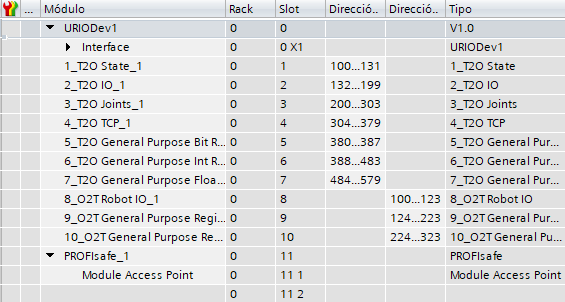
\includegraphics[width=15cm]{figs/com_ur_modulos}
  \end{center}
  \caption{\centering Configuración de los módulos de comunicación del UR en Tia Portal.}
  \label{fig:com_ur_modulos}
\end{figure} 

\clearpage

\begin{figure} [h!]
  \begin{center}
    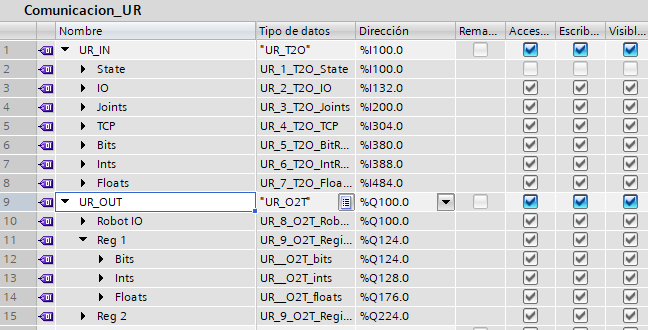
\includegraphics[width=13cm]{figs/com_plc_ur}
  \end{center}
  \caption{\centering Configuración de los módulos de comunicación del UR en Tia Portal.}
  \label{fig:com_plc_ur}
\end{figure} 

Finalmente, una vez que las estructuras de datos definidas por el usuario permiten mapear adecuadamente los registros de entrada y salida del robot, se pueden modificar los registros booleanos, enteros o flotantes para enviarle información desde el PLC al UR. Los datos que el PLC envía al UR se escriben en las direcciones asignadas a las salidas (UR\_OUT.Reg 1), mientras que los datos recibidos del UR se leen desde las direcciones de entrada (UR\_IN). Cuando la comunicación entre el robot y el PLC se establece con éxito, el LED del controlador del robot cambia a verde como se observa en la siguiente imagen:

\begin{figure} [h!]
  \begin{center}
    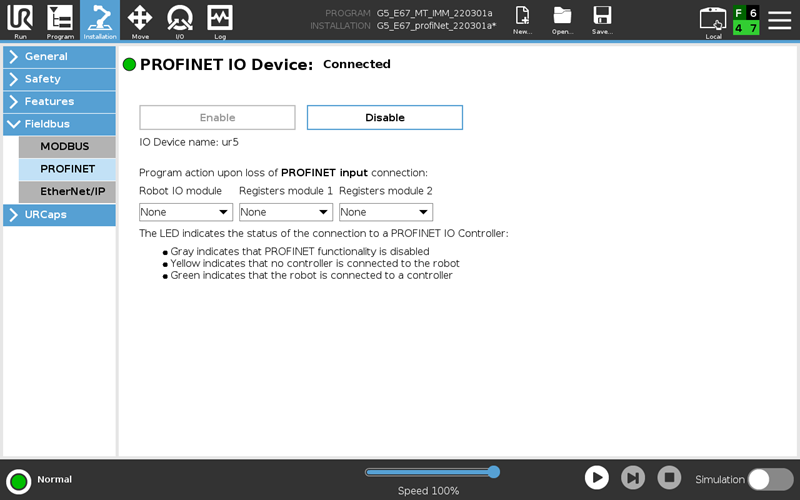
\includegraphics[width=12cm]{figs/ur_conectado_plc}
  \end{center}
  \caption{\centering Conexión establecida entre el UR y el PLC. \cite{guia_profinet}}
  \label{fig:ur_conectado_plc}
\end{figure} 

Seguidamente se muestra una tabla que resume todos los mensajes intercambiados entre los dispositivos en el ciclo global: 

\newcolumntype{M}[1]{>{\centering\arraybackslash}m{#1}}

\begin{table}[H]
\begin{center}

\renewcommand{\arraystretch}{1.5}
\begin{tabular}{|M{1.75cm}|M{1.75cm}|M{3.5cm}|M{7.5cm}|}
\hline
\textbf{Emisor} & 
\textbf{Receptor} & 
\textbf{Mensaje} & 
\textbf{Explicación} \\
\hline
PLC 1  & PLC 2 &  \makecell{Send\_fase\_1  \\ (Bool)} & Se envía si el tipo de pieza es aceptado y pasa de la estación distribución a la estación unión. \\
\hline
PLC 2  & PLC 1 &  \makecell{Send\_fase\_1  \\ (Bool)} & Confirmación de que la pieza pasó exitosamente de la estación distribución a la estación unión. \\
\hline
PLC 1  & PLC 2 &  \makecell{Tipo\_de\_pieza   \\ (Int)} &  \makecell{Indica el tipo de pieza detectado: \\ Pieza negra: 1 \\ Pieza rosa: 2 \\ pieza metálica: 3}  \\
\hline
PLC 2  & PLC 1 &  \makecell{Secuencia\_acabada  \\ (Bool)} &  Se le indica a la estación unión que la estación distribución terminó su ciclo con éxito. \\
\hline
PLC 1  & PLC 2 &  \makecell{Secuencia\_ACK   \\ (Bool)} &  Confirmación de la recepción del mensaje Secuencia\_acabada. \\
\hline
PLC 2  & PLC 1 &  \makecell{Pieza\_mal\_orientada   \\ (Bool)} &  Se le indica a la estación unión que la pieza actual está mal orientada y se debe descartar. \\
\hline
PLC 1  & PLC 2 &  \makecell{Pieza\_mal\_ACK  \\ (Bool)} &  Confirmación de la recepción del mensaje Pieza\_mal\_orientada. \\
\hline
PLC 1  & UR5e &  \makecell{Start \\ Registro GPbi [0] \\ (Bool)} & Indica el inicio de la secuencia de colocación de la pieza en el palé del UR. \\
\hline
PLC 1  & UR5e  &  \makecell{num\_capas \\ Registro GPii [0] \\ (Int)} & Número de capas elegido en el HMI que se quieren para el paletizado. \\
\hline
Ur5e  & PLC 1 &  \makecell{piezas\_paletizadas \\ Registro GPio [0] \\ (Int)} & Número de piezas paletizadas actualmente. \\
\hline
UR5e   & PLC 1 &  \makecell{ejecutando\_proc \\ Registro GPbo [0] \\ (Bool)} & Informa que el UR todavía está ejecutando su ciclo. \\
\hline
UR5e   & PLC 1 &  \makecell{pale\_completo \\ Registro GPbo [1] \\ (Bool)} & Aviso de que el palé está completo. \\
\hline
PLC 1  & UR5e  &  \makecell{pale\_recogido  \\  Registro GPbi [2] \\ (Bool)} & Informa de que el palé ha sido recogido. \\
\hline
UR5e   & PLC 1 &  \makecell{Pale\_ACK \\ Registro GPbo [2] \\ (Bool)} & Confirmación de la recepción del mensaje pale\_recogido. \\
\hline
PLC 1  & UR5e  &  \makecell{parada\_emergencia  \\  Registro GPbi [1] \\ (Bool)} & Parada de emergencia pulsada, parada obligatoria de la secuencia. \\
\hline
\end{tabular}

\caption{Intercambio de mensajes en el ciclo global del sistema.}
\label{cuadro:mensajes}
\end{center}
\end{table}
 
\section{Funcionamiento estación distribución}
\label{sec:funcionamiento_distribucion}

La estación distribución es la encargada de iniciar la secuencia del proceso automático. Está conectada al primer PLC y tiene como función principal suministrar piezas al sistema, ya sea a través de su cinta transportadora o mediante el dispensador de piezas. Además, el usuario puede seleccionar desde el HMI el tipo de material de la pieza para permitir o no su paso. También se establece un número máximo de piezas permitidas; una vez alcanzado este límite, se bloquea el paso de nuevas piezas hasta que el contador sea reiniciado, como medida de control y revisión del proceso. En caso de que la pieza no cumpla con las condiciones establecidas en la interfaz de usuario, esta será devuelta al inicio del recorrido y descartada. Si cumple los requisitos, continuará su avance hacia la siguiente estación. Adicionalmente se ha implementado un modo de prueba que permite verificar el funcionamiento individual de cada sensor y actuador, facilitando así la detección de posibles errores. A continuación, se presenta una tabla que recoge todas las entradas y salidas de la estación, así como su correspondencia con las conexiones al PLC:

\begin{table}[H]
\begin{center}

% Tabla 1 (Sensores)
\begin{tabular}{|P{6.5cm}|P{4cm}|P{2.5cm}|}
\hline
\multicolumn{1}{|c|}{\textbf{Sensor}} & 
\multicolumn{1}{c|}{\textbf{Entrada al PLC}} & 
\multicolumn{1}{c|}{\makecell{\textbf{Tipo de salida} \\ \textbf{(normalmente)}}} \\
\hline
Láser inicio cinta  & \%I0.0 &  abierta \\
Láser medio cinta  & \%I0.1 &  abierta \\
Láser final cinta  & \%I0.2 &  cerrada \\
Identificador de piezas (pieza negra)  & \%I0.4 &  abierta \\
Sensor de color (pieza rosa)  & \%I0.5 &  abierta \\
Sensor metálico (pieza metálica)  & \%I0.6 &  abierta \\
Corredera retraída  & \%I0.7 &  abierta \\
Corredera extendida & \%I1.0 &  abierta \\
Pieza en el cargador & \%I1.1 &  cerrada \\
\hline
\end{tabular}

\vspace{0.2cm}

% Tabla 2 (Actuadores)
\begin{tabular}{|P{6.95cm}|P{6.95cm}|}
\hline
\multicolumn{1}{|c|}{\textbf{Actuador}} & 
\multicolumn{1}{c|}{\textbf{Salida del PLC}} \\
\hline
Avance cinta & \%Q0.0 \\
Retroceso cinta & \%Q0.1 \\
Separador & \%Q0.2 \\
Avance corredera & \%Q0.3 \\
\hline
\end{tabular}

\caption{Entradas y salidas de la estación distribución conectadas al PLC 1}
\label{cuadro:distribucion}
\end{center}
\end{table}

El Grafcet de la figura \ref{fig:grafcet_distribucion} describe la secuencia automatizada de funcionamiento de la estación de unión. El sistema se inicializa con la variable de conteo de piezas a cero y permanece en espera hasta recibir una orden de arranque desde la interfaz HMI. En función del modo de carga seleccionado (manual o automático), se introduce la pieza en el sistema por la parte inicial de la cinta transportadora (donde será necesario activar el separador para permitir su paso) o a través de la corredera que realiza un movimiento de extensión y retracción para depositar la pieza retenida en el cargador. A continuación, se lleva a cabo una etapa de identificación en la que se determina el tipo de pieza (negra, rosa o metálica), registrándose dicha información en el sistema y actualizándose el contador de piezas correspondiente. \\

 El HMI cuenta con una interfaz para seleccionar el tipo de pieza que se quiere aceptar y la que se quiere descartar, como se observa en la imagen \ref{fig:HMI_funcionamiento}, con la configuración mostrada, los tres tipos de piezas serían descartados. Si se ha alcanzado el número total de piezas especificado por el operador o el tipo de pieza no está permitida por el operario, el sistema ejecuta un retroceso de la cinta para descartar la pieza y repetir el ciclo hasta que se reseté el contador de piezas o se amplíe el número desde el HMI. Puede haber otro caso de descarte en la estación unión, por lo que si sucede, el PLC 1 recibirá un mensaje de error procedente del PLC 2 comunicándole que le devuelve la pieza expulsándola por la zona inicial de la cinta y terminando el ciclo global. \\
 
En el caso de que no ocurra ningún imprevisto, se da por finalizado el proceso de carga de la pieza en el sistema al recibir un mensaje del PLC 2 de que la pieza pasó a su estación con éxito. Posteriormente se envía una señal al PLC 2 para confirmar la recepción de su mensaje, y a continuación, se procede a comunicarle al robot UR el inicio de su secuencia de colocación de la pieza en el palé (siempre y cuando no esté colocando ya una pieza, que en ese caso esperará a que acabe). Esta comunicación se realiza mediante la activación de un registro booleano global a través del canal PROFINET, acompañado por un registro entero que indica el número de capas de paletizado (de 1 a 4) que se quieren realizar definidas previamente en el HMI. En este punto hay dos posibles estados diferentes a los que transitar, si el UR indica que está ejecutando su secuencia, se da por terminado el ciclo global y se inicia de nuevo permitiendo comenzar el siguiente ciclo sin la necesidad de esperar a que el brazo termine su proceso. Por otro lado, si el UR indica que el palé está completo, salta un aviso en la pantalla del HMI para retirarlo como se observa en la figura \ref{fig:HMI_funcionamiento_UR_recoger} la cual ya se explicará más adelante. Tras retirar el palé, se pulsa el botón correspondiente en el HMI y, al recibir el mensaje de confirmación (ACK), el ciclo concluye.

\clearpage

\begin{figure} [h!]
  \begin{center}
    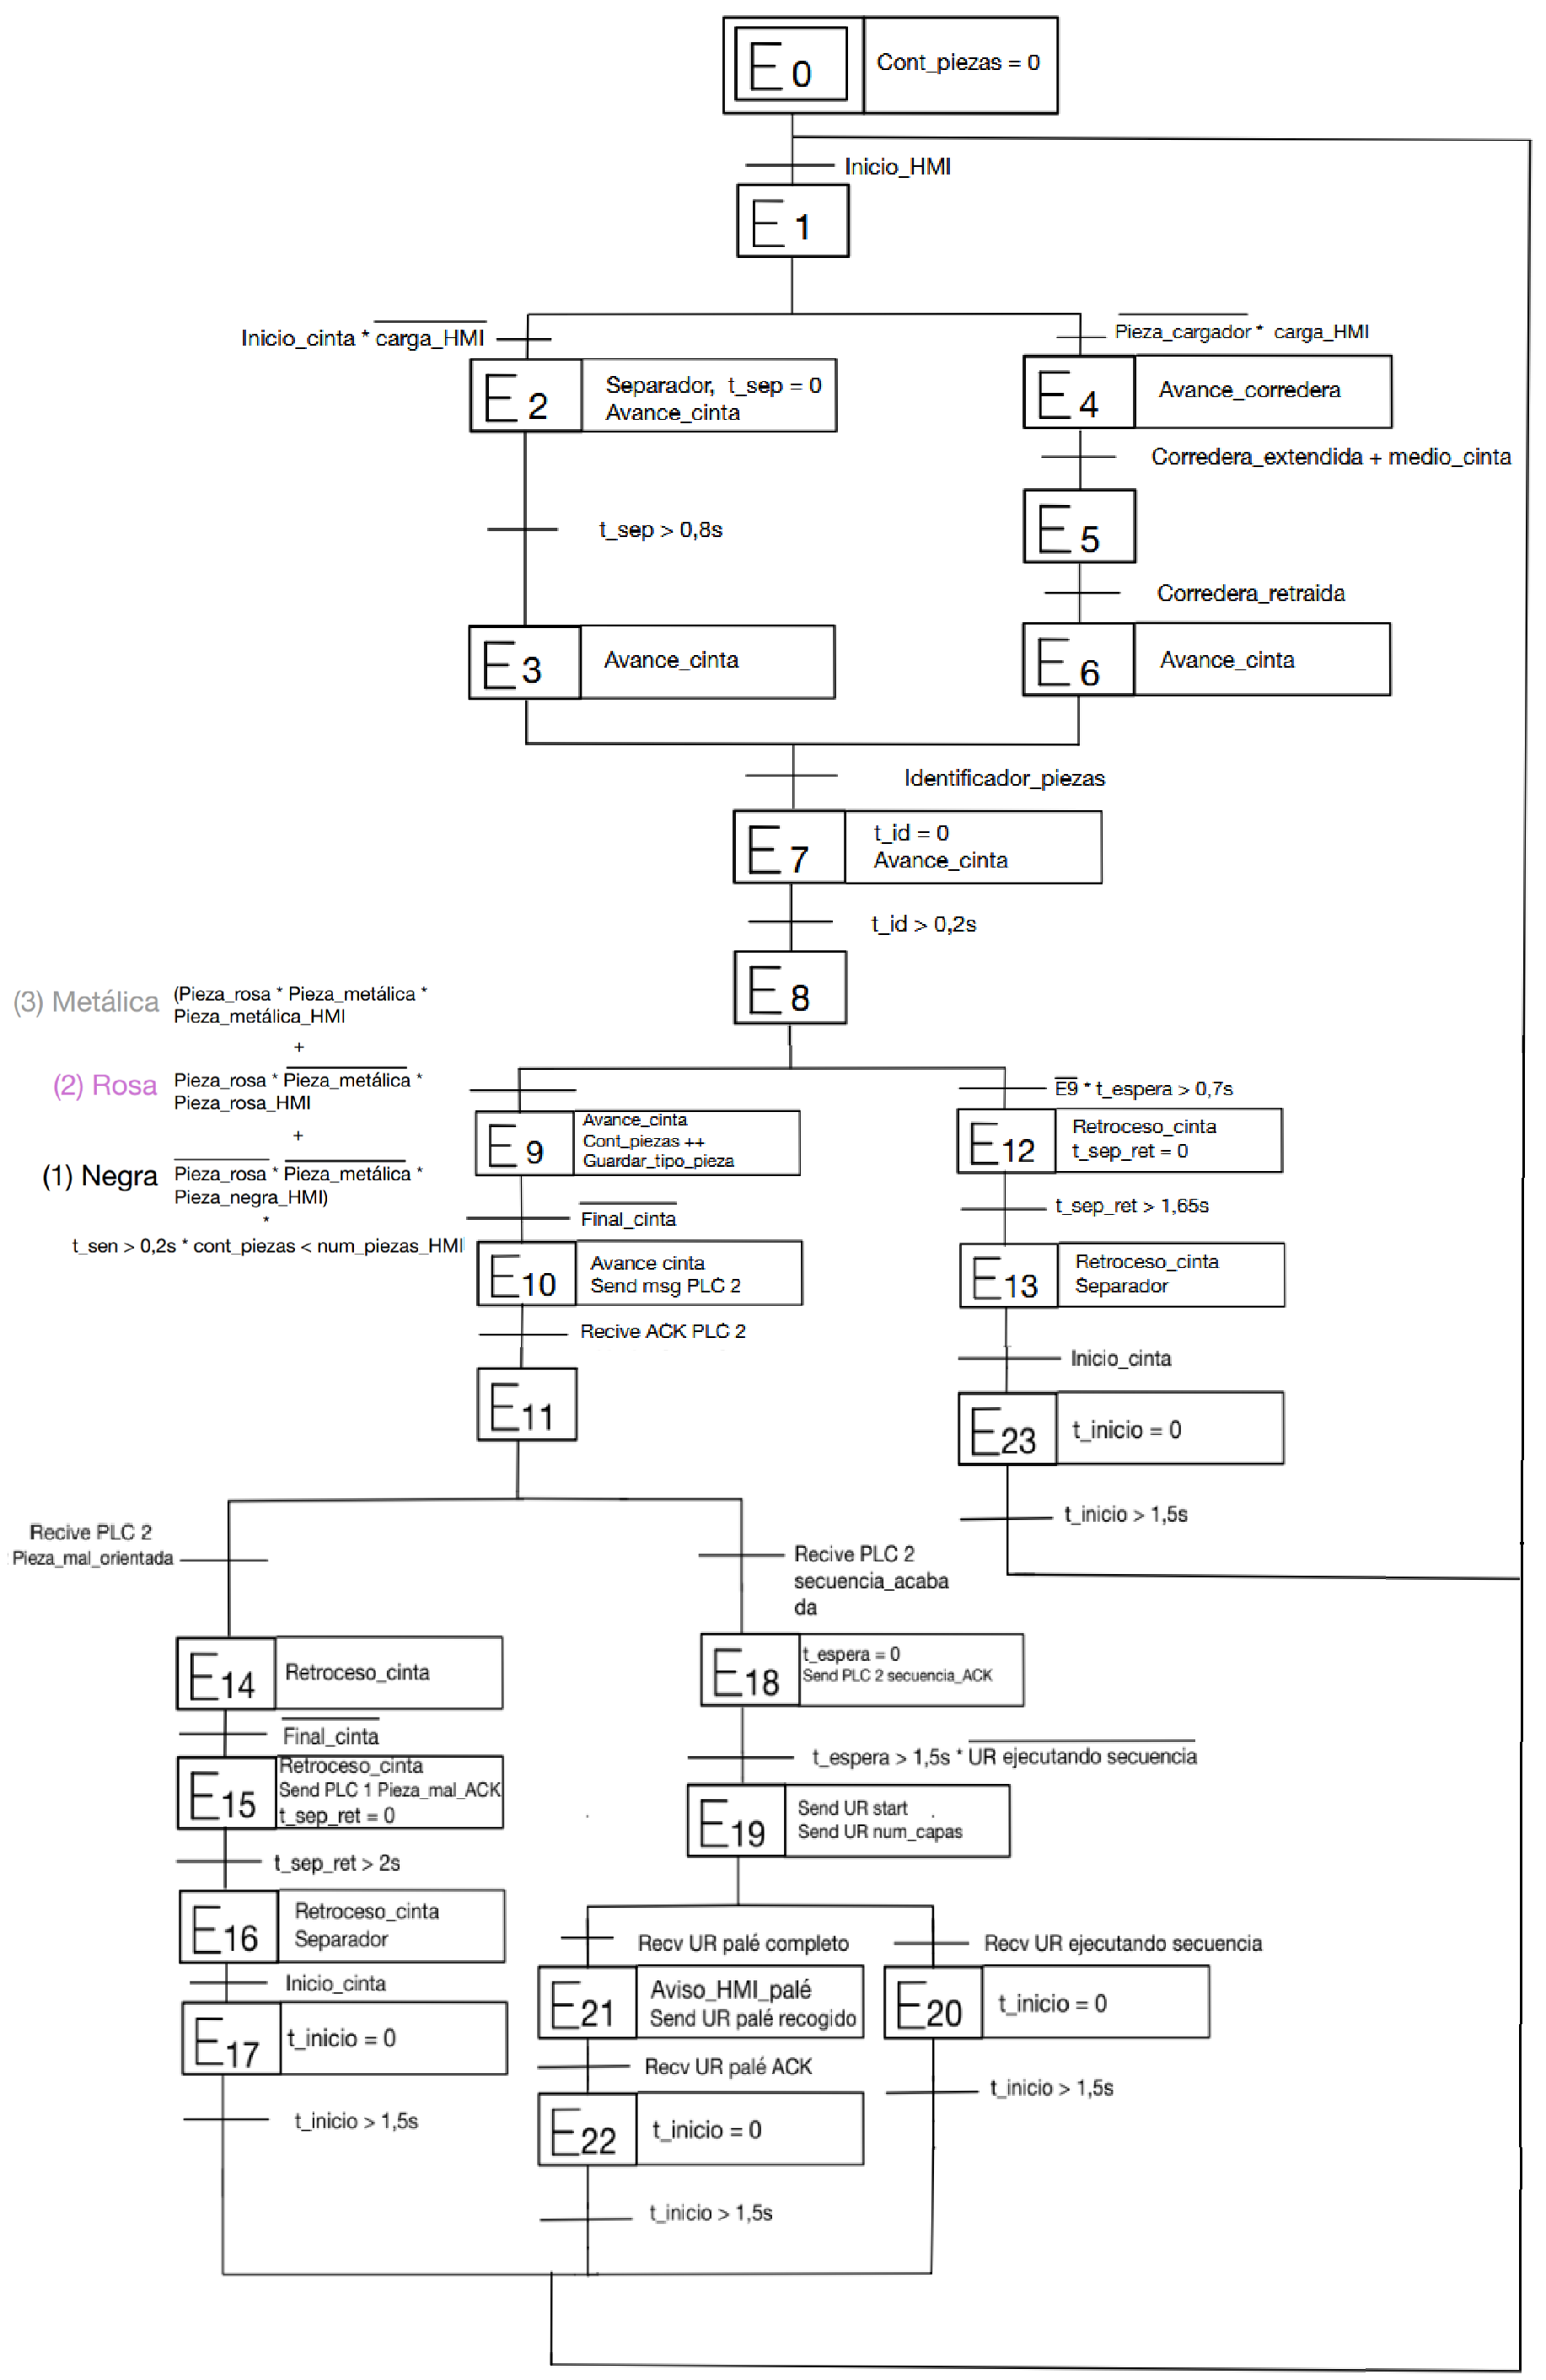
\includegraphics[width=14cm]{figs/grafcet_distribucion}
  \end{center}
  \caption{\centering Grafcet del funcionamiento de la estación distribución.}
  \label{fig:grafcet_distribucion}
\end{figure} 

En el anexo \ref{sec:anexo_distribucion} se detallan las ecuaciones lógicas del Grafcet de la estación distribución.

\clearpage

\begin{figure} [h!]
  \begin{center}
    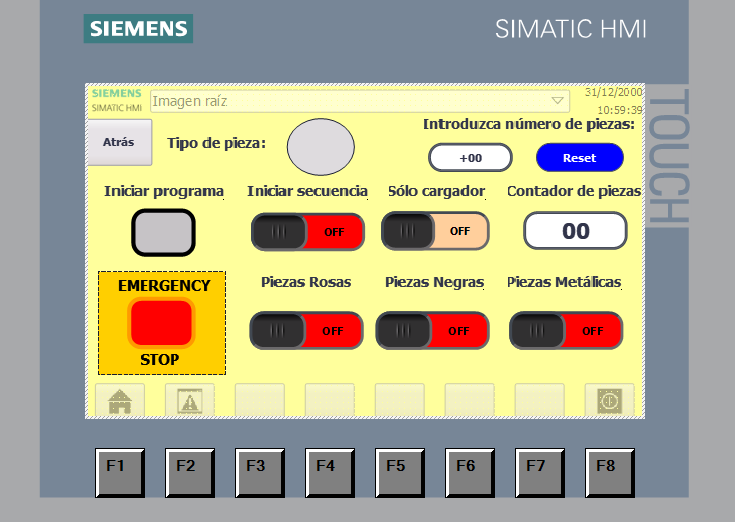
\includegraphics[width=13.5cm]{figs/HMI_funcionamiento}
  \end{center}
  \caption{\centering Pantalla del modo funcionamiento en el HMI.}
  \label{fig:HMI_funcionamiento}
\end{figure} 


En la foto anterior se muestra la pantalla del modo funcionamiento del sistema, en la que cada botón tiene el siguiente funcionamiento:

\begin{itemize}
    \item \textbf{Número de capas:} Introducir el número de capas de paletizado deseado, siendo 1 el mínimo y 4 el máximo de capas debido a la restricción física del espacio de trabajo del cobot.
    
    \item \textbf{Número de piezas:} Introducir el número de piezas que se desean permitir en el proceso. El botón azul ``Reset `` reinicia el contador a 0.
    
    \item \textbf{Iniciar programa:} Inicia el programa después de una parada de emergencia.
    
    \item \textbf{Iniciar secuencia:} Inicia la secuencia global de producción.
    
    \item \textbf{Sólo cargador:} Indica que sólo se quieren utilizar piezas provenientes del cargador. De lo contrario, las piezas serán introducidas al sistema desde el inicio de la cinta transportadora.
    
    \item \textbf{Contador de piezas:} Muestra un contador con el número de piezas producidas hasta el momento.
    
    \item \textbf{Parada de emergencia:} Botón de seguridad que provoca que todos los elementos del proceso se paren instantáneamente.
    
    \item \textbf{Piezas Rosas:} Permite el paso de piezas rosas, de lo contrario se descartan.
    
    \item \textbf{Piezas Negras:} Permite el paso de piezas negras, de lo contrario se descartan.
    
    \item \textbf{Piezas Metálicas:} Permite el paso de piezas metálicas, de lo contrario se descartan.

\end{itemize}

\begin{figure}[h!]
  \begin{center}
  	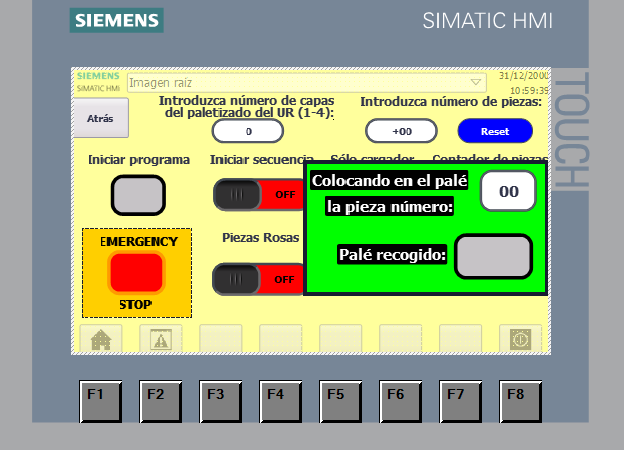
\includegraphics[width=15cm]{figs/HMI_funcionamiento_UR_recoger}
  \end{center}
  \caption{\centering Botón utilizado para la confirmación de que el palé ha sido recogido en la pantalla de funcionamiento del HMI.}
  \label{fig:HMI_funcionamiento_UR_recoger}
\end{figure}

En la figura anterior se presenta una captura de pantalla del HMI en modo de funcionamiento, mostrando un mensaje que indica que el UR está colocando la \textbf{última pieza} del palé, parando el resto del sistema hasta que le botón ``Palé recogido'' sea pulsado. Al pulsar este botón, y siempre que el UR haya finalizado correctamente la colocación de dicha pieza, se envía una señal de confirmación al brazo robótico para verificar que el palé ha sido recogido de forma segura. Esto permite que la producción continúe sin interrupciones, garantizando la coordinación y seguridad en la línea de ensamblaje.

\clearpage

\section{Funcionamiento estación unión}
\label{sec:funcionamiento_union}

La estación de unión es la encargada de ensamblar las diferentes piezas que llegan desde la estación anterior, la cual se encuentra conectada al segundo PLC del sistema y tiene como objetivo principal la unión de una base con una tapa, verificando previamente que ambas piezas estén correctamente posicionadas. El proceso de unión se lleva a cabo mediante un actuador neumático equipado con una ventosa, el cual puede desplazarse entre las dos cintas transportadoras para ascender o descender con el fin de recoger o depositar las tapas. En caso de que alguna de las piezas se encuentre mal posicionada, el sistema detiene el ciclo, notifica el error a través de un mensaje mostrado en la pantalla del HMI y descarta la pieza afectada. Esta estación, al igual que la estación de distribución, dispone de un modo de prueba que permite revisar de forma individual el funcionamiento de cada sensor y actuador, lo cual facilita la identificación de posibles fallos. A continuación, se presentan la tabla \ref{cuadro:union}, en la que se detallan todas las entradas y salidas de la estación, así como su correspondiente conexión con el PLC.

\begin{table}[H]
\begin{center}

% Tabla 1 (Sensores)
\begin{tabular}{|P{6.5cm}|P{4cm}|P{2.5cm}|}
\hline
\multicolumn{1}{|c|}{\textbf{Sensor}} & 
\multicolumn{1}{c|}{\textbf{Entrada al PLC}} & 
\multicolumn{1}{c|}{\makecell{\textbf{Tipo de salida} \\ \textbf{(normalmente)}}} \\
\hline
Láser inicio cinta 1 & \%I0.0 &  abierta \\
Láser medio cinta 1  & \%I0.1 &  abierta \\
Láser final cinta 1  & \%I0.2 &  cerrada \\
Orientación correcta  & \%I0.3 &  abierta \\
Láser final cinta 2 & \%I0.4 &  abierta \\
Láser inicio cinta 2 & \%I0.5 &  cerrada \\
Carro retraído & \%I0.6 &  abierta \\
Carro extendido & \%I0.7 &  abierta \\
Ventosa arriba & \%I1.0 &  abierta \\
Pieza succionada & \%I1.1 &  abierta \\

\hline
\end{tabular}

\vspace{0.2cm}

% Tabla 2 (Actuadores)
\begin{tabular}{|P{6.95cm}|P{6.95cm}|}
\hline
\multicolumn{1}{|c|}{\textbf{Actuador}} & 
\multicolumn{1}{c|}{\textbf{Salida del PLC}} \\
\hline
Avance cinta 1 & \%Q0.0 \\
Retroceso cinta  2 & \%Q0.1 \\
Extender separador & \%Q0.2 \\
Retraer tope & \%Q0.3 \\
Avance cinta 2 & \%Q0.4 \\
Retroceso cinta 2 & \%Q0.5 \\
Retroceso carro & \%Q0.6 \\
Avance carro & \%Q0.7 \\
Bajar ventosa & \%Q1.0 \\
Vacío conectado & \%Q1.1 \\
\hline
\end{tabular}

\caption{Entradas y salidas de la estación unión conectadas al PLC 2}
\label{cuadro:union}
\end{center}
\end{table}

El Grafcet de la estación distribución se muestra en la figura \ref{fig:grafcet_union}, cuyo proceso inicia activando el avance de la cinta 1 al recibir un mensaje del PLC 1 hasta que la pieza proveniente de la estación distribución es detectada por el láser del inicio, luego se envía un mensaje de confirmación de que la pieza llegó al segundo sistema. La cinta continúa moviéndose hasta que la pieza es detectada en el centro de la cinta por el segundo láser y se extiende el retenedor para poder así comprobar correctamente la orientación de la pieza. A continuación se verifica la orientación de la pieza utilizando un sensor capacitivo: si la pieza está correctamente orientada, el sensor no la detecta, mientras que si está invertida, el sensor la activa, indicando una orientación incorrecta. Hay que tener en cuenta que si se trata de una pieza metálica, el sensor tiene el comportamiento opuesto, detectándose en caso de que esté correctamente orientada, por lo que en el Grafcet se han tenido que establecer las condiciones específicas para las piezas de este material. Si se confirma que la orientación es válida, paralelamente se dan dos sucesos: en el primero se vuelve a activar la cinta 1, se extiende el derivador y se espera el tiempo necesario para que la pieza llegue hasta este último y el segundo consiste en que la cinta 2 avanza hasta que en el láser del inicio de esta detecta una tapa. \\

Una vez la pieza está parada y la tapa lista para recogerse, el carro se extiende, desciende la ventosa, succiona la pieza, se eleva y se retrae colocándola encima. Después la ventosa se desactiva, se activa la cinta 1 nuevamente y se retrae el separador permitiendo a la pieza llegar al final de la cinta, que, cuando es detectada por el último láser, manda un mensaje al PLC 1 indicando que la secuencia ha terminado. Si la orientación es incorrecta, se activa un proceso de rechazo y una notificación al operario en el HMI mostrando un mensaje y contador de piezas defectuosas. El sistema esperará hasta que el operario pulse el botón de “descartar pieza” como se ve en la imagen \ref{fig:HMI_descarte}. Una vez pulsado, se activa el retroceso de la cinta y el envío de un mensaje de error al PLC 1 avisando que debe descartar la pieza. El ciclo finaliza tras la confirmación de recepción de la secuencia completada o de pieza defectuosa por parte del PLC 1.

\clearpage
 
 \begin{figure}[h!]
  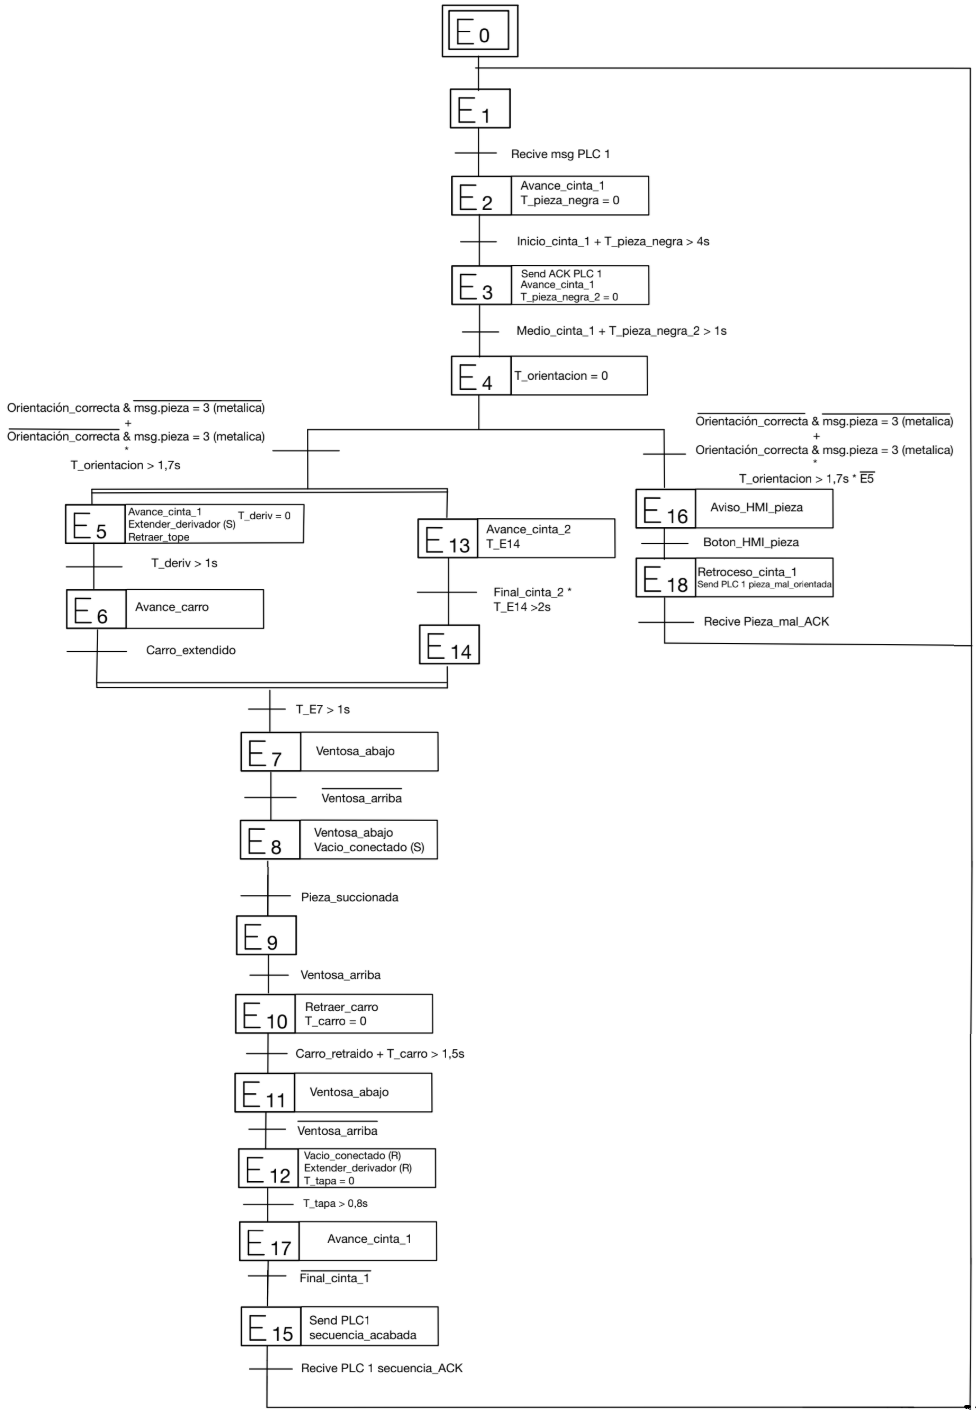
\includegraphics[width=15cm]{figs/grafcet_union}
  \caption{\centering Grafcet de funcionamiento de la estación unión.}
  \label{fig:grafcet_union}
\end{figure}

En el anexo \ref{sec:anexo_union} se detallan las ecuaciones lógicas del Grafcet de la estación distribución.

\clearpage

\begin{figure}[h!]
  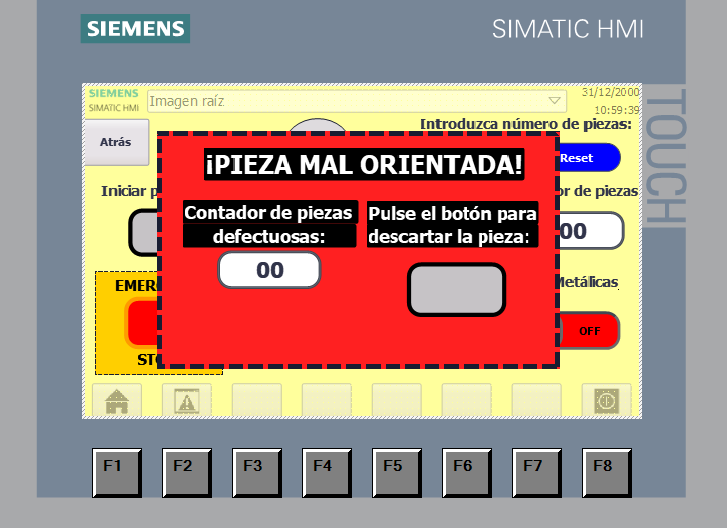
\includegraphics[width=15cm]{figs/HMI_descarte}
  \caption{\centering Aviso de pieza defectuosa en el modo funcionamiento en el HMI.}
  \label{fig:HMI_descarte}
\end{figure}

\section{Aplicación de la Guía GEMMA}
\label{sec:aplicacion_gemma}

La aplicación de la Guía GEMMA, explicada previamente en la sección \ref{sec:terceraseccion}, representa un elemento clave en el desarrollo de sistemas automatizados, especialmente en entornos industriales. En el contexto del proyecto, la Guía GEMMA ha sido de gran utilidad para estructurar de forma lógica y ordenada las distintas acciones que componen el ciclo global de producción. Gracias a su enfoque, ha sido posible identificar de manera precisa las condiciones iniciales, las etapas activas del proceso y las posibles interrupciones. Esta clasificación favorece la implementación de programas más robustos y fácilmente mantenibles, además de mejorar la comprensión del funcionamiento general del sistema por parte de otros desarrolladores o técnicos. Para su correcta aplicación, se han definido y utilizado en el proyecto los siguientes estados operativos:

\begin{table}[H] 
\begin{center}

\renewcommand{\arraystretch}{1.5}
\begin{tabular}{|P{3.5cm}|P{4cm}|P{7cm}|}
\hline
\textbf{Modo} & \textbf{Tipo} & \textbf{Objetivo} \\
\hline

\multirow{2}{=}{Proceso de funcionamiento} 
    & F1: Producción normal & Se realizan las tareas principales del sistema. \\
\cline{2-3}
    & F4: Marchas de verificación sin orden & Se realiza un control manual de los actuadores y la comprobación del funcionamiento de los sensores. \\
\hline

\multirow{3}{=}{Proceso de parada o puesta en marcha} 
    & A1: Parada en el estado inicial & Estado de reposo de la máquina. \\
\cline{2-3}
    & A2: Parada solicitada al final de ciclo & Estado al que se llega  cuando se termina el ciclo y pasa al estado inicial\\
\cline{2-3}
    & A3: Parada solicitada en un estado determinado & Estado al que llega la máquina alternativo el cual no coincide con el final de ciclo. \\
\cline{2-3}
    & A4: Parada obtenida & Estado de reposo diferente al principal. \\
\cline{2-3}
    & A5: Puesta en marcha después de defecto & Estado posterior a un defecto y necesario para restablecer el sistema. \\
\hline

Proceso en defecto & D1: Parada de emergencia & Estado al que llega el sistema tras una parada de emergencia. Se para el funcionamiento de todo el sistema. \\
\hline

\end{tabular}

\caption{Estados de la Guía GEMMA utilizados en el sistema.}
\label{cuadro:union}
\end{center}
\end{table}

\subsubsection{Proceso de funcionamiento}

En el proceso de funcionamiento hay configurados dos estados distintos, El primer estado es el F1 o producción normal, estado en el que el sistema repite constantemente el ciclo de producción que ha sido programado. En este estado y como se puede observar en la figura \ref{fig:HMI_funcionamiento}, se pueden configurar los parámetros del sistema desde el HMI con aspectos clave como: seleccionar el tipo de pieza que se quiere dejar pasar, introducir el número de piezas que se quieren producir,  iniciar o parar la secuencia o decidir si se quiere utilizar el cargador o no. El sistema estará dentro de este estado principal, siempre y cuando no surja algún imprevisto o comportamiento extraño.

En cuanto al estado F4 o marcha de verificación sin orden, tiene como objetivo realizar un control manual de los actuadores y sensores para comprobar su correcto funcionamiento. Para este estado se han creado dos modos de test a cada estación física (distribución y unión, Estos modos de pruebas son seleccionables en el menú principal del HMI antes de entrar en el estado de producción F1 como se aprecia en la imagen \ref{fig:HMI_inicio}. Una vez dentro del modo test, y por lo tanto, dentro del estado F4, se puede acceder a una vista de diagnóstico de errores general o  se puede escoger entre el modo de pruebas de la estación distribución o unión. La estación distribución sólo cuenta con un modo test, en cambio la estación unión cuenta con dos modos debido a que tiene más sensores y actuadores para probar el funcionamiento.

\begin{figure}[H]
  \centering

  \begin{minipage}{0.8\textwidth}
    \centering
    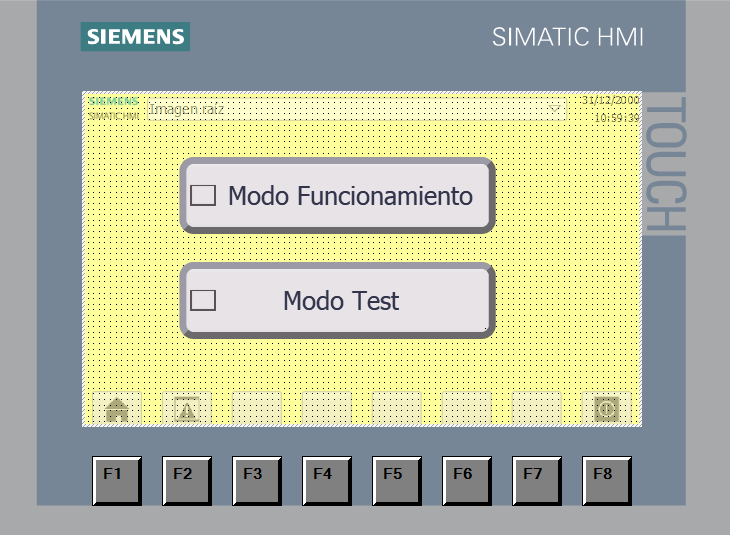
\includegraphics[width=\textwidth]{figs/HMI_inicio}
    \captionof{figure}{\centering Estado inicial del HMI.}
    \label{fig:HMI_inicio}
  \end{minipage}
  \hfill
  \begin{minipage}{0.8\textwidth}
    \centering
    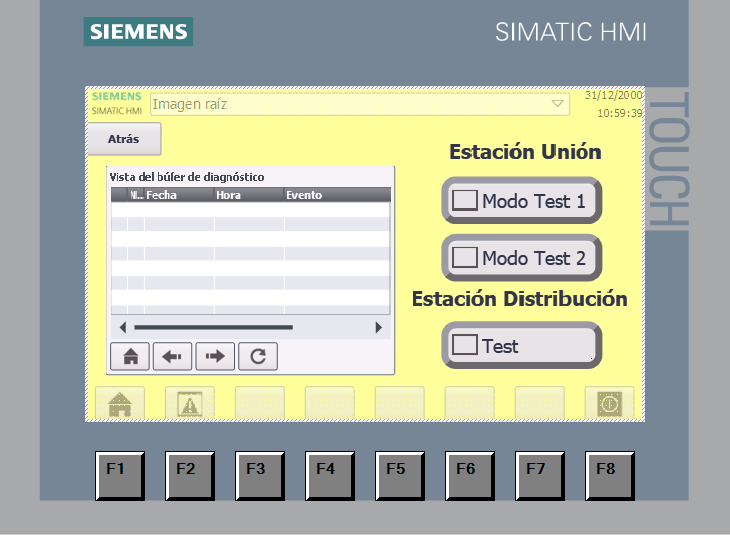
\includegraphics[width=\textwidth]{figs/HMI_test_principal}
    \captionof{figure}{\centering Vista del HMI dentro de la opción Modo Test.}
    \label{fig:HMI_test_principal}
  \end{minipage}

\end{figure}
\clearpage

En la figura \ref{fig:HMI_test_distribucion} se pueden ver todos los test que se le pueden realizar en la estación distribución. Es posible activar y desactivar manualmente los actuadores del sistema, como la cinta transportadora, el separador o el cargador, con el fin de verificar su correcto funcionamiento. Además, se muestran tres columnas y tres filas de círculos que representan visualmente todos los sensores de la estación de distribución, así como el tipo de pieza detectado por el módulo adicional de dicha estación. Cuando un sensor está activo, su indicador aparece en verde; en caso contrario, se muestra en rojo. En cuanto al tipo de pieza, solo se activa el correspondiente al detectado durante el ciclo de trabajo en curso. Esta visualización facilita la comprobación del estado de los sensores y permite monitorizar el proceso para detectar posibles errores como se muestra en la siguiente imagen: 

\begin{figure}[h!]
  \begin{center}
  	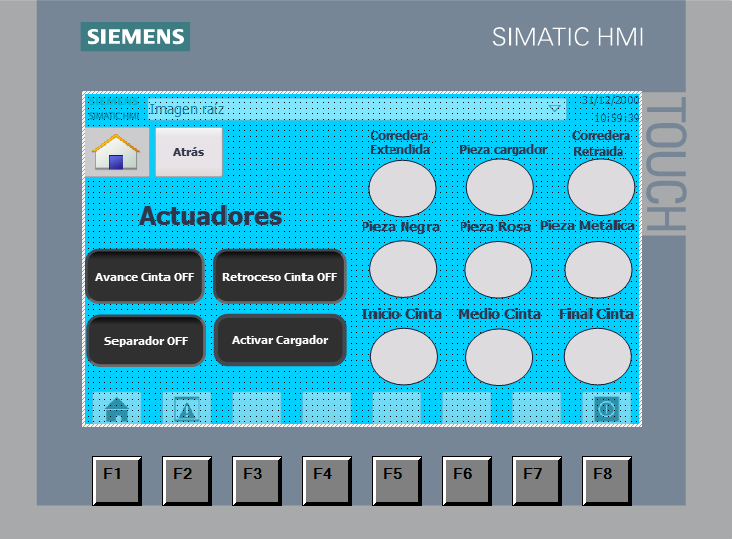
\includegraphics[width=12cm]{figs/HMI_test_distribucion}
  \end{center}
  \caption{\centering Visualización del modo Test de la estación distribución dentro del HMI.}
  \label{fig:HMI_test_distribucion}
\end{figure}

Por otro lado, el modo test de la estación de unión se ha distribuido en dos pantallas distintas, ya que el elevado número de sensores y actuadores impide representarlos todos de forma clara en una sola vista. La estructura de este modo sigue el mismo esquema que en la estación de distribución: se emplean botones para activar o desactivar los actuadores, y se utilizan círculos de colores para indicar visualmente el estado de los sensores. Un círculo verde señala un sensor activo, mientras que el rojo indica que está desactivado y también se cuenta con un botón que al presionarlo el HMI abre la pantalla del otro test programado para esta estación. A continuación se muestra el modo test para la estación unión:

\begin{figure}[H]
  \centering

  \begin{minipage}{0.95\textwidth}
    \centering
    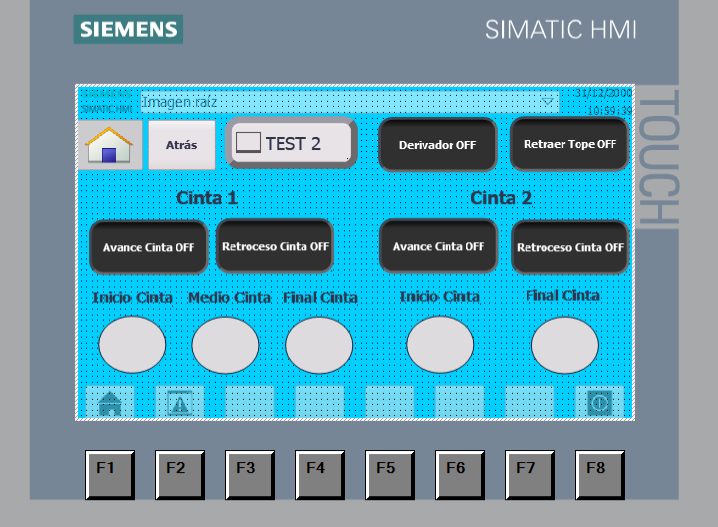
\includegraphics[width=\textwidth]{figs/HMI_test_union_1}
    \captionof{figure}{\centering Vista del HMI dentro de la opción Modo Test 1 de la estación unión.}
    \label{fig:HMI_test_union_1}
  \end{minipage}
  \hfill
  \begin{minipage}{0.95\textwidth}
    \centering
    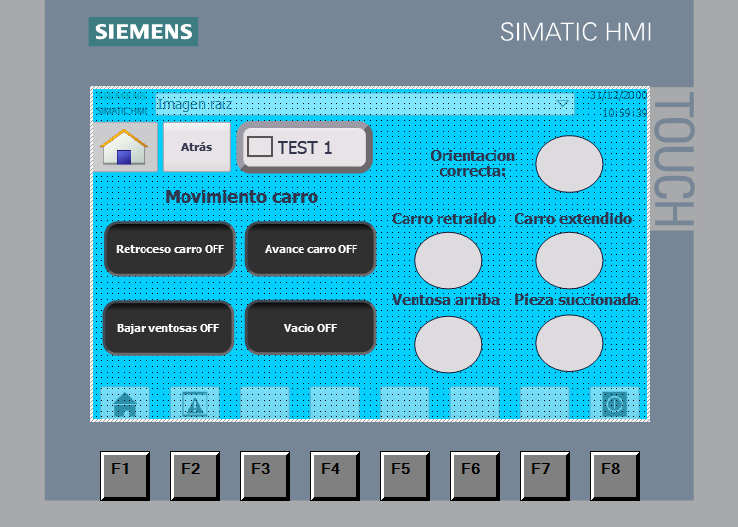
\includegraphics[width=\textwidth]{figs/HMI_test_union_2}
    \captionof{figure}{\centering Vista del HMI dentro de la opción Modo Test 2 de la estación unión.}
    \label{fig:HMI_test_union_2}
  \end{minipage}
\end{figure}


\subsubsection{Proceso de parada o puesta en marcha}

Este conjunto de estados definidos por la Guía GEMMA describe las distintas situaciones en las que una máquina puede encontrarse durante la detención o reactivación del proceso. Son fundamentales para garantizar transiciones seguras y controladas entre ciclos de funcionamiento. A continuación, se explican los cuatro estados que componen este proceso:

\begin{itemize}
    \item \textbf{A1: Parada en el estado inicial} \\
    Representa el estado de reposo principal de la máquina. Es el punto de partida al que se regresa tras completar un ciclo \cite{guia_gemma}. En este estado, no hay procesos activos y la máquina está lista para comenzar un nuevo ciclo de forma segura una vez se pulse dentro de la interfaz del HMI el botón ``Iniciar secuencia''.

    \item \textbf{A2: Parada solicitada al final de ciclo} \\
    Este estado funciona como transición entre la producción normal del sistema a la parada del estado inicial cuando se termina el ciclo principal \cite{guia_gemma}. Cada vez que el sistema termina su ciclo, se queda parado y transiciona al estado A1 de forma automática para volver a empezar la secuencia. Esta parada permite volver al estado inicial de parada una vez ha terminado el ciclo de producción si no está activado el botón ``iniciar secuencia'' en el HMI, permitiendo así parar el ciclo de producción.
    
    \item \textbf{A3: Parada solicitada en un estado determinado} \\
    Corresponde a una parada anticipada, en un punto concreto del ciclo, distinto del final \cite{guia_gemma}. Se emplea cuando es necesario interrumpir el proceso en un estado específico, por razones de control, mantenimiento o condiciones externas \cite{guia_gemma}. Este estado se alcanza cuando le llega a la estación unión una pieza mal orientada, por lo que el estado se queda detenido hasta que el operario descarta la pieza en el HMI, la imagen \ref{fig:HMI_descarte} representa este estado. También existe otra forma de alcanzar este estado, la cual ocurre cuando el UR ha colocado la última pieza del palé y el sistema queda en espera hasta que el operario retire el palé manualmente. Posteriormente, el operario debe pulsar el botón “palé recogido” para que el proceso continúe, tal como se muestra en la figura \ref{fig:HMI_funcionamiento_UR_recoger}. \\

    \item \textbf{A4: Parada obtenida} \\
    Indica que la máquina ha alcanzado un estado de reposo diferente al inicial A1 y proveniente del A3 \cite{guia_gemma}. Este estado alternativo está asociado a situaciones específicas, como pruebas, diagnóstico o pausas no planificadas \cite{guia_gemma}. Esta parada se activa al cumplirse cualquiera de las dos condiciones descritas en el estado A3, ambas necesarias para garantizar un funcionamiento seguro y correcto del sistema.
    
   \item \textbf{A5: Puesta en marcha después de defecto} \\
   En este estado se realizan las acciones necesarias para la reanudación del correcto funcionamiento del sistema después de un defecto \cite{guia_gemma}. \\
   A este estado se llegará después de una parada de emergencia y será necesario pulsar el botón ``iniciar programa'' en la interfaz HMI de modo funcionamiento para transicionar al estado A1.
\end{itemize}

\subsubsection{Proceso en defecto}

Dentro del proceso de defecto sólo se ha programado el estado D1 de parada de emergencia. Este estado representa una situación crítica en la que el sistema se detiene de forma inmediata debido a una emergencia \cite{guia_gemma}. La parada se realiza sin esperar a que finalice el ciclo, con el objetivo de garantizar la seguridad de las personas, del sistema o del entorno \cite{guia_gemma}. Este estado puede ser alcanzado en cualquier momento que se presione el botón ``parada de emergencia'' desde el HMI en el modo de funcionamiento. Una vez pulsado el botón se para el funcionamiento de todo el sistema para ser revisado por un operario, y una vez resuelto el problema, se podrá volver a comenzar con el ciclo de producción desde 0.

\subsubsection{Aplicación de la Guía GEMMA}

Una vez descritos en detalle todos los posibles estados que puede adoptar el sistema a lo largo de su funcionamiento, se presenta a continuación la imagen \ref{fig:guia_gemma_final} muestra gráficamente todas las transiciones entre dichos estados. Esta representación visual resulta especialmente útil para comprender de forma global el comportamiento del sistema automatizado en sus distintas fases operativas. 

\clearpage

\begin{figure}[h!]
  \begin{center}
  	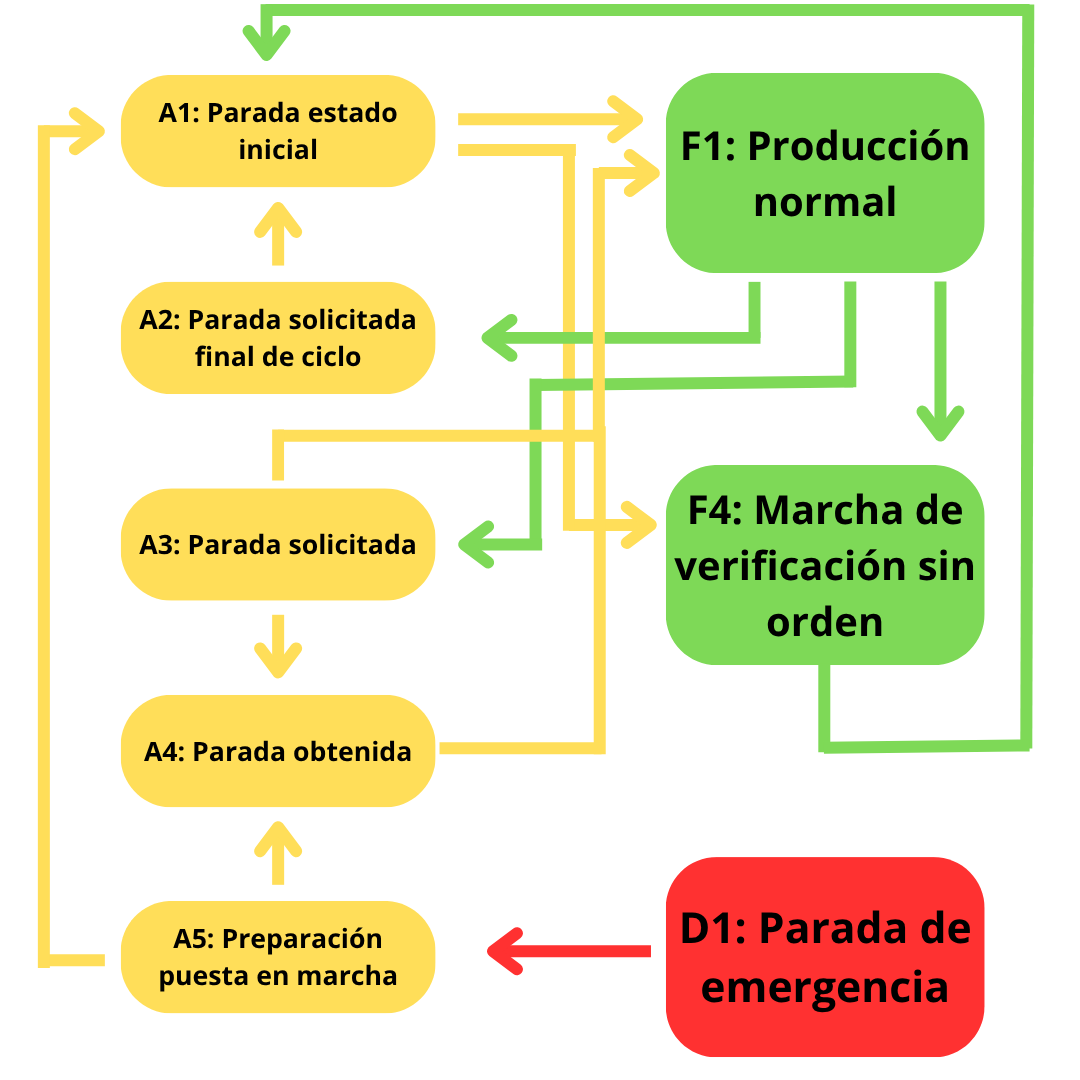
\includegraphics[width=16.5cm]{figs/guia_gemma_final}
  \end{center}
  \caption{\centering Esquema de transiciones de la aplicación de la Guía GEMMA en el sistema.}
  \label{fig:guia_gemma_final}
\end{figure}

En la figura, los elementos de color verde corresponden al proceso de funcionamiento normal, los de color amarillo al proceso de parada o de puesta en marcha, y los de color rojo al proceso de detección de defectos o fallos. La imagen también cuenta con una leyenda explicando las acciones necesarias para transicionar entre estados.

\clearpage

\section{Funcionamiento cobot UR5e}
\label{sec:funcionamiento_ur5e}

El cobot UR5e es un brazo robótico colaborativo diseñado para trabajar de forma segura junto a operarios. En este proyecto, su función principal es comunicarse con los PLCs para ejecutar una secuencia de paletizado en la fase final del ciclo global del sistema. Una vez que la estación de unión completa su ciclo, el PLC 1 envía una señal al UR5e indicándole que inicie su secuencia. Al finalizar la operación de colocación de la pieza en el palé, el cobot notifica al PLC 1 que ha concluido, permitiendo así reiniciar el ciclo completo. El propósito de integrar el brazo en la ejecución del sistema es simular su uso dentro del proceso automático (aunque físicamente no se pudo integrar debido a la distancia entre estaciones) para ordenar las piezas , aportando así mayor realismo y complejidad al resultado final. 

El cobot viene equipado con una pinza neumática como herramienta. Esta pinza permite sujetar, mover y soltar objetos de forma rápida y eficiente. Es ideal para tareas repetitivas como ensamblaje, paletizado, manipulación de piezas o carga de máquinas, especialmente cuando no se requiere un control preciso de la fuerza. Esta pinza se ha utilizado para la secuencia de paletizado, la cual sigue el esquema llamado \textbf{paletizado por capas}. Este tipo de paletizado por capas consiste en organizar productos sobre un palé formando niveles horizontales uniformes agrupando varios elementos alineados o alternos para lograr estabilidad \cite{paletizado_capas}. Es ideal para cargas regulares y facilita la automatización, optimizando espacio, transporte y manipulación en entornos industriales \cite{paletizado_capas}. 

\begin{figure}[h!]
  \begin{center}
  	\includegraphics[width=11.5cm]{figs/brazo_pinza}
  \end{center}
  \caption{\centering UR5e junto con la pinza como herramienta.}
  \label{fig:brazo_pinza}
\end{figure}

Como ya se ha visto en la sección \ref{sec:conectividad_dispositivos}, el PLC 1 le envía un mensaje al UR para iniciar el programa de paletizado. En este programa se ha utilizado la herramienta de paletizado integrada en Polyscope. Esta funcionalidad permite crear un palé de cualquier tipo de elemento indicando únicamente el número de capas deseadas y las coordenadas de la posición de cada uno. Tal como se ha mencionado anteriormente, se ha llevado a cabo un paletizado por capas, utilizando bricks de leche como elementos a colocar, simulando una secuencia real en un entorno industrial. Se han configurado cuatro capas en total: dos con una disposición determinada y las otras dos con una diferente, obteniendo el siguiente resultado:

\begin{figure}[h!]
  \begin{center}
  	\includegraphics[width=14.5cm]{figs/resultado_paletizado}
  \end{center}
  \caption{\centering Resultado final del paletizado de bricks de leche por el UR5e.}
  \label{fig:resultado_paletizado}
\end{figure}

Las coordenadas de la posición de las piezas en el paletizado se han tomado de forma relativa a la coordenada del primer brick de leche. La primera coordenada se definió en la posición que se quería colocar el primer elemento del palé, y a partir de esta y tomándola de referencia, se han definido las 5 coordenadas restantes. Al utilizar el sistema de coordenadas del primer punto se han podido colocar elementos paralelos y perpendiculares al primero, ayudando a aportar gran estabilidad y orden al palé. Esta técnica también ha ayudado mucho a establecer la misma altura de todos los bricks de leche y asegurarse así que no se coloquen de forma uniforme. Adicionalmente, se han establecido algunos puntos de paso también utilizando este sistema de coordenadas para intentar establecer los movimientos lo más rectilíneos posibles. Seguidamente se muestra una tabla que refleja las coordenadas de las posiciones de cada pieza que forman el palé, tomando como referencia la primera posición para definir el resto de ellas:

\begin{table}[H]
\begin{center}

\renewcommand{\arraystretch}{1.5}
\begin{tabular}{|M{2.45cm}|M{2.65cm}|M{1.2cm}|M{1.2cm}|M{1.2cm}|M{1.1cm}|M{1.1cm}|M{1.1cm}|}
\hline
\textbf{Coordenada de la pieza} &
\textbf{Sistema de coordenadas} & 
\textbf{X (mm)} & 
\textbf{Y (mm)} & 
\textbf{Z (mm)} &
\textbf{RX (rad)} &
\textbf{RY (rad)} &
\textbf{RZ (rad)} \\
\hline
Posición 1  & Base UR5e &  -333,6 & 270,9 & 70,0 & 0 & 3,15 & 0 \\
\hline
Posición 2  & Posición 1 &  0 & -128 & 0 & 0 & 0 & 0 \\
\hline
Posición 3  & Posición 1 &  198,3 & -82,3 & 0 & 0 & 0 & 1,57 \\
\hline
Posición 4  & Posición 1 &  -43,3 & -24,8 & 0 & 0 & 0 & 4,71 \\
\hline
Posición 5  & Posición 1 &  90 & 0 & 0 & 0 & 0 & 0 \\
\hline
Posición 6  & Posición 1 &  90 & -128 & 0 & 0 & 0 & 0 \\
\hline
\end{tabular}

\caption{\centering Coordenadas de colocación de las piezas en el palé utilizando el UR5e.}
\label{cuadro:coordenadas}
\end{center}
\end{table}

En cuanto a la comunicación PROFINET entre el UR y el PLC 1 ya explicada en la sección \ref{sec:conectividad_dispositivos}, se han utilizado los siguientes registros de propósito general para el intercambio de información en los mensajes entre ambos:

\begin{table}[H]
\begin{center}

\renewcommand{\arraystretch}{1.5}
\begin{tabular}{|M{3.4cm}|M{2.3cm}|M{3cm}|M{2.5cm}|M{2cm}|}
\hline
\textbf{Nombre variable} &
\textbf{Número de registro} & 
\textbf{Direcci\'on para el UR5e} & 
\textbf{Direcci\'on para el PLC} &
\textbf{Tipo de dato} \\
\hline
Start  & GPbi [0] & Entrada & Salida & Bool \\
\hline
parada\_emergencia  & GPbi [1] & Entrada & Salida & Bool \\
\hline
pale\_recogido  & GPbi [2] & Entrada & Salida & Bool \\
\hline
num\_capas  & GPii [0] & Entrada & Salida & Int \\
\hline
piezas\_paletizadas  & GPio [0] & Salida & Entrada  & Int \\
\hline
ejecutando\_proc  & GPbo [0] & Salida & Entrada & Bool \\
\hline
pale\_completo  & GPbo [1] & Salida & Entrada & Bool \\
\hline
pale\_ACK  & GPbo [2] & Salida & Entrada & Bool \\
\hline

\end{tabular}

\caption{Registros utilizados para la comunicación entre el UR5e y el PLC 1.}
\label{cuadro:registros}
\end{center}
\end{table}

En el cuadro \ref{cuadro:mensajes} ya se ha explicado el objetivo y significado de la utilización de estos registros en el código del UR; sin embargo, en este apartado se va a profundizar aún más en su funcionamiento, describiendo detalladamente la lógica implementada, comentando el código del brazo robótico que se muestra a continuación, y explicando cómo se gestionan las señales de comunicación y sincronización de tareas.

\begin{code}[h]
\begin{lstlisting}[]
# AntesDeIniciar
Ajustar ejecutando_proc= False
capa_controller := 0
contador_piezas := 0
num_capas := numero_capas*3
if num_capas>12
    num_capas:=12

# Programa de robot
Bucle num_capas>contador_piezas:
    Ajustar pale_completo= False
    Ajustar pale_ACK= False
    Moverj
        Punto_inicio
    # Esperar al mensaje de inicio del PLCs
    Esperar: start:=Hi
    if contador_piezas + 1 >= num_capas:
        Ajustar pale_completo= True
    Else:
        Ajustar ejecutando_proc= True
    Ajustar piezas_paletizadas= contador_piezas + 1
    # Coger pieza
    Moverj
        Recogida_alto
        Recogida_leche
        Ajustar_pinza := Encender
        Esperar: 1.5
        Recogida_alto
    # Punto de paso de coordenada 3
    if capa_controller == 2
        Moverj
            base_colocar_3
    # Punto de paso de coordenada 4
    Elseif capa_controller == 3:
        Moverj
            base_colocar_1
            base_colocar_2
    # Punto de paso del resto de coordenadas
    Else:
        Moverj
            base_colocar_1
    # Coordenadas de las posiciones de las piezas
    Pallet
        Irregular Pattern 1
            Item_1
            Item_2
            Item_3
        Irregular Pattern 2
            Item_4
            Item_5
            Item_6
\end{lstlisting}
\caption[Programa de robot en Polyscope]{\centering Programa del UR5e exportado desde Polyscope.}
\label{cod:prog_ur_1}
\end{code}

\clearpage

\begin{code}[h]
\begin{lstlisting}[]
    # Dentro de la capa actual
    Capas
        for articulo in articulos:
            Moverj
                ToolActionPoint
            MoverL
                ToolActionPoint
            # Soltar la pieza
            Tool action
                Ajustar pinza= Apagar
                Esperar: 1.0
            MoverL
                if capa_controller != 3
                    Exit
    # En la coordenada 4 subir de forma manual
    if capa_controller == 3:
        MoverL
            Salida_coord_4
    # Actualizar contadores
    capa_controller += 1
    contador_piezas += 1
    if capa_controller > 5:
        capa_controller := 0
    Ajustar ejecutando_proc= False
# Fin del programa (pale completado)
contador_piezas := 0
capa_controller := 0
Moverj
    Punto_inicio
Esperar: pale_recogido:=Hi
Ajustar pale_ACK= True
Esperar: 1.0

\end{lstlisting}
\caption[Programa de robot en Polyscope]{\centering Programa del UR5e exportado desde Polyscope.}
\label{cod:prog_ur_2}
\end{code} 

\FloatBarrier

El código del UR5e define un programa de control que ejecuta un ciclo de recogida y colocación de piezas en distintas coordenadas de un palé. Al inicio, se inicializan variables de control: \texttt{ejecutando\_proc} se pone en falso, \texttt{capa\_controller} y \texttt{contador\_piezas} se inicializan en cero, y se calcula \texttt{num\_capas} multiplicando \texttt{numero\_capas} (información leída del registro GPii [0] cuyo valor es introducido por el operario en el HMI) por tres debido a que cada capa consta de tres elementos, limitándolo a un máximo de 12.

El programa del robot se repite en bucle constantemente, y dentro de él, el ciclo principal se ejecuta siempre y cuando \texttt{contador\_capas} sea menor que \texttt{num\_capas}. Dentro del bucle, se inicializan los registros \texttt{pale\_completo} y \texttt{pale\_ACK} con el valor cero para indicar al PLC que el robot UR está a la espera de la orden de inicio. A continuación, el robot se desplaza a la posición de inicio para quedar preparado y, cuando el PLC activa el registro \texttt{start}, el programa verifica si la pieza a colocar corresponde a la última del palé o no. En caso afirmativo, se activa el registro \texttt{pale\_completo} para indicar al sistema que, una vez colocada esta pieza, el palé debe ser retirado por estar completo mediante un mensaje en el HMI como se observa en la figura \ref{fig:HMI_funcionamiento_UR}. Si no se trata de la última pieza, se activa el registro \texttt{ejecutando\_proc} para indicar al PLC que el UR ha iniciado su ciclo. Para terminar la comunicación inicial de la secuencia, se le indica al PLC a través del registro \texttt{piezas\_paletizadas} el número de pieza que está siendo colocada en ese momento, mostrándose en la pantalla del HMI como se observa en la siguiente imagen:

\begin{figure}[h!]
  \begin{center}
  	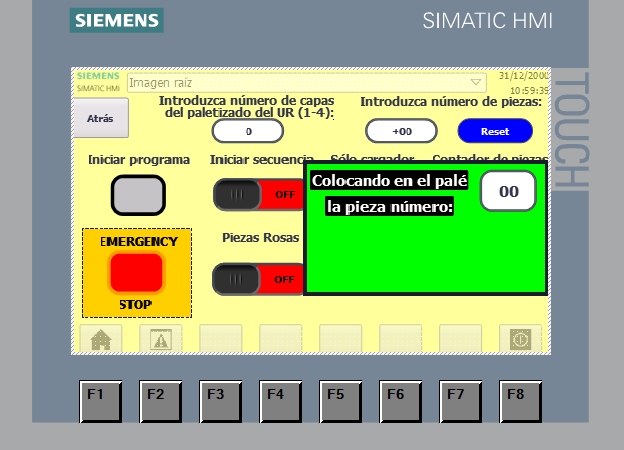
\includegraphics[width=15cm]{figs/HMI_funcionamiento_UR}
  \end{center}
  \caption{\centering Mensaje del número pieza siendo colocada por el UR en la pantalla de funcionamiento del HMI.}
  \label{fig:HMI_funcionamiento_UR}
\end{figure}

Una vez la comunicación con el PLC realizada, el robot se aproxima a la posición de recogida de piezas, baja con cuidado hasta la pieza, activa la pinza para agarrarla, espera 1,5 segundos y la sube ligeramente. Siempre que el brazo lleva la pieza sujeta se mueve más lento que cuando no la tiene, de esta manera, según el valor de \texttt{capa\_controller} (la posición de la pieza actual), el robot ajusta su trayectoria para pasar por distintas coordenadas definidas para optimizar el recorrido. Estos puntos de paso que sigue el UR5e también han sido definidos utilizando la posición de la coordenada 1 de colocación de la pieza como referencia para conseguir trayectorias lo más seguras posibles.

Luego, mediante la estructura de datos del palé previamente definida, el robot coloca las piezas en posiciones específicas dentro de la capa actual. En el momento que el brazo coloca la pieza en su posición, abre la pinza y sube hacia arriba en línea recta para no golpear a las demás piezas ya colocadas. En el caso de la pieza 4, el brazo ejecuta un movimiento programado manualmente para elevarse, ya que, al hacerlo de forma automática, el TCP quedaba demasiado cerca del codo del robot, lo que provocaba la activación del estado de parada de emergencia por razones de seguridad.

Después, se actualizan los contadores de piezas y capa, si se supera el valor a cinco, el controlador de capa se reinicia (ya han sido colocadas todas las piezas en las dos capas). También se desactiva el registro \texttt{ejecutando\_proc} para indicar que la pieza ya ha sido colocada finalizando así el ciclo del UR.

Si el UR ya ha colocado todas las piezas en sus respectivas coordenadas y el palé está completo, se resetean los contadores, se mueve a su posición de inicio y se queda esperando a que el PLC le confirme que el palé ha sido retirado con éxito. En el momento que le llega el mensaje, cuando el operario presione el botón ``Palé recogido'' en el HMI de la figura \ref{fig:HMI_funcionamiento_UR}, le confirma la recepción del mismo a través de la activación del registro \texttt{pale\_ACK} y esperará 1 segundo para asegurarse de que la información le llega correctamente al PLC. El estado de espera del UR cuando el palé ha sido completado ha sido diseñado para aportar seguridad al sistema, asegurándose de que no coloca una nueva pieza cuando todavía no se ha retirado el palé anterior, si se dispusiese de una cinta transportadora se podría retirar el palé automáticamente en vez de forma manual. 

\section{Resultado final}
\label{sec:resultado_final}

En este apartado se presentan los resultados finales obtenidos tras el desarrollo e implementación del proyecto. Se incluyen vídeos demostrativos en los que se puede observar el funcionamiento del sistema automático industrial en condiciones reales de operación. Estos vídeos ilustran el comportamiento del proceso completo, mostrando cómo el sistema responde a las diferentes señales de control, coordina sus componentes y ejecuta de forma autónoma las tareas para las que fue diseñado. 

\clearpage

\subsubsection{Funcionamiento global del sistema}

\textbf{Vídeo:} \url{https://youtu.be/a00Lm__qqNk} \\

Este vídeo muestra el ciclo global del sistema funcionando correctamente, sin presentar ningún imprevisto. En él se integran las dos estaciones junto con el robot UR. Según la configuración establecida, el sistema acepta 10 piezas como máximo, todo tipo de materiales y se quiere formar pales de 2 capas de altura. Las piezas son dispensadas por el cargador, pasan por la estación de unión para la colocación de las tapas y finalmente llegan al extremo de la cinta transportadora. En un momento del vídeo se observa que, cuando la tercera pieza está lista para recibir la tapa pero no hay ninguna disponible, el sistema permanece en espera hasta que una nueva tapa es suministrada para poder continuar con el proceso. 

Cuando la pieza llega al final de la cinta, comienza la secuencia del robot UR, que simula la recogida y  colocación de la pieza en la posición correspondiente para formar el palé. En la pantalla del HMI aparece un mensaje sobre la secuencia en curso. Además, antes de finalizar este ciclo, se inicia un nuevo ciclo global, optimizando el tiempo al permitir que una nueva pieza entre al sistema mientras se coloca la anterior. El ciclo global se ejecuta seis veces hasta completar el paletizado, momento en el que aparece en el HMI el mensaje de "recoger el pale". En el vídeo se muestra cómo se pulsa dicho botón antes de que el UR coloque la última pieza, sin embargo, el sistema no responde hasta que el brazo termina de colocar la pieza. En ese instante, al pulsar el botón y confirmar la retirada del palé, el ciclo comienza nuevamente desde el inicio. \\

En el vídeo se observan dos pequeños problemas de hardware independientes a este proyecto, ya que son debidos a un mal montaje de la estación unión, realizada por terceras personas. El primer error está en el separador (encargado de frenar la pieza para poder colocar la tapa encima suya), ya que no se retrae nunca del todo y provoca que la pieza no pueda alcanzar el último láser de la cinta transportadora. El segundo error está en el brazo que coloca la tapa encima de la pieza, que en algún momento no la suelta en la parte central de la pieza dejándola un poco suelta debido a que no está bien configurado. 

\clearpage



\subsubsection{Funcionamiento estación distribución}

\textbf{Vídeo:} \url{https://youtu.be/nUW7nG6U8uE} \\

En el vídeo se observa el funcionamiento de la estación distribución junto con la interfaz del HMI. El primer paso consiste en pulsar el botón “iniciar programa”, ya que el sistema se encontraba previamente en estado de parada de emergencia, y al hacerlo, se transiciona al estado inicial. El proceso inicia cuando se pulsa el botón ``iniciar secuencia'', pero la pieza rosa no es aceptada por el sistema porque el botón ``Piezas rosas'' está desactivado. Una vez se activa, se observa como la pieza ahora si es aceptada, pero otra de otro material como la metálica se descarta hasta que se activa su respectivo botón ``Piezas metálicas''. Finalmente, se cambia el valor del contador de piezas, pasando de permitir 8 piezas a 0, por lo que aunque se permita el paso de todo tipo de materiales de piezas, no lo harán ya que no cumplen la condición del número máximo de piezas permitido. \\

\subsubsection{Descarte de pieza mal orientada}

\textbf{Vídeo:} \url{https://youtu.be/pbC6FhVJhaw} \\

Este ejemplo se enfoca en el funcionamiento de la detección de la orientación de las piezas en la estación unión. En este caso una pieza rosa llega hasta el sensor capacitivo después de pasar los filtros de la estación distribución, pero al detectar que su orientación no es la correcta (está al revés y la tapa no puede colocarse encima de ella) es descartada. Cuando su orientación incorrecta es detectada por el sensor, salta un mensaje en el HMI mostrando el contador de piezas defectuosas y el botón para descartarla. Hasta que el botón no es pulsado el sistema se queda en espera, y una vez presionado, la pieza es descartada pasando por la estación distribución. Después se ejecuta otra vez la secuencia con la pieza bien orientada y esta vez si es aceptada por el sistema y continúa con su ciclo. 

\clearpage

\subsubsection{Secuencia de paletizado completa}

\textbf{Vídeo:} \url{https://youtu.be/vDtNlI_9-sc} \\

El vídeo muestra la secuencia completa de paletizado realizada por el robot UR. En esta demostración se omite el proceso de las dos estaciones para enfocarse exclusivamente en el paletizado de las piezas, partiendo de la premisa de que estas llegan correctamente posicionadas para que el brazo las recoja. El sistema está configurado para realizar cuatro capas de paletizado, que es el máximo permitido. Se puede observar que las capas 1 y 3 presentan la misma disposición, mientras que las capas 2 y 4 tienen una configuración distinta que complementa a las anteriores, formando una estructura más sólida en comparación con otras configuraciones posibles. \\

\subsubsection{Parada de emergencia}

\textbf{Vídeo:} \url{https://youtu.be/WvFtP7whsRg} \\

Este último ejemplo ilustra una situación de parada de emergencia. En le vídeo se observa que, una vez iniciado el ciclo global, el sistema opera con normalidad hasta que se activa el botón “parada de emergencia”, lo que provoca la detención inmediata de todo el proceso y de todos los actuadores. En este estado, todos los elementos del sistema quedan bloqueados para permitir la identificación y resolución del fallo que originó la parada. Una vez solucionada la incidencia, se debe pulsar nuevamente el botón “iniciar programa” para retornar al estado inicial de parada.

En el vídeo se muestra una repetición de la secuencia, esta vez interrumpida mediante una parada de emergencia justo en el momento en que el robot UR se encuentra ejecutando su secuencia de paletizado. Tal como se observa, al pulsar el botón “parada de emergencia” desde el HMI, el UR recibe la orden de abortar el programa a través del registro \texttt{GPbi[1]}, finalizando inmediatamente su operación.




\chapter{Conclusiones}
\label{cap:capitulo5}

\begin{flushright}
\begin{minipage}[]{10cm}
\emph{La robótica industrial convierte lo imposible en rutinario}\\
\end{minipage}\\

Anónimo\\
\end{flushright}

\vspace{1cm}

En este último capítulo se presenta una síntesis de todo el trabajo realizado a lo largo de este proyecto. Se repasan los principales problemas abordados, las soluciones propuestas para cada uno de ellos y los experimentos desarrollados para validar dichas soluciones. Este capítulo ofrece una visión global de los retos enfrentados, los resultados obtenidos y las conclusiones derivadas del proceso de diseño, implementación y evaluación de la automatización industrial estudiada.


\section{Conclusiones}

Durante el desarrollo de este trabajo se ha logrado cumplir con todos objetivos propuestos: se ha llevado a cabo el montaje, conexionado y validación del sistema completo en condiciones reales, comprobando su funcionamiento y fiabilidad. Se ha automatizado el funcionamiento de las estaciones didácticas mediante la programación en TIA Portal, implementando una lógica de control robusta. Se ha diseñado y configurado una interfaz HMI que permite al operario controlar el sistema y supervisar sus estados en tiempo real, facilitando su trabajo y proporcionando una abstracción de bajo nivel que simplifica la interacción con los procesos automatizados. Se ha integrado con éxito el robot colaborativo UR5e en el flujo de trabajo, realizando operaciones de paletizado coordinadas. Además, se ha creado una red de comunicaciones PROFINET entre PLCs, HMI y el cobot, asegurando un intercambio de datos fiable y continuo. Por último, la lógica de control secuencial se ha desarrollado utilizando Grafcet y la guía GEMMA como referencia metodológica, integrándose de manera coherente con el resto de la programación y contribuyendo a garantizar un funcionamiento ordenado y seguro del sistema. \\

A lo largo de este trabajo, se ha conseguido desarrollar un sistema de automatización integral que reúne control, comunicación y robótica colaborativa, lo que representa un avance significativo respecto al estado inicial, donde los procesos estaban fragmentados y carecían de integración eficiente. La implementación de una red PROFINET y la utilización de metodologías estructuradas como Grafcet y GEMMA han permitido mejorar la coordinación y fiabilidad del sistema, facilitando su escalabilidad y mantenimiento. Además, se ha logrado programar y dejar preparadas las estaciones físicas en el laboratorio para que puedan servir como plataforma de pruebas y aprendizaje para futuras generaciones de estudiantes que cursen asignaturas relacionadas con este ámbito, facilitando su comprensión de la materia y ofreciéndoles un entorno práctico para desarrollar sus competencias. 

No obstante, el sistema presenta ciertas limitaciones, como la separación física entre las estaciones y el robot colaborativo, lo que impide una integración completa del brazo robótico en el proceso de producción y limita su capacidad para recoger las piezas utilizadas en las estaciones durante la secuencia de paletizado. Además, la complejidad de la integración entre diferentes dispositivos obliga a un conocimiento especializado para su operación y mantenimiento. A nivel personal, este proyecto ha sido una oportunidad valiosa para profundizar en la programación industrial de PLCs y del brazo robótico, protocolos de comunicación y diseño de interfaces, consolidando habilidades prácticas y teóricas que serán fundamentales en mi desarrollo profesional.

De cara al futuro, este trabajo podría ampliarse integrando nuevas estaciones de producción o adaptando el sistema para entornos industriales reales con mayor variabilidad y exigencia de seguridad tanto física como virtual. También sería posible profundizar en la optimización de las secuencias de paletizado y en la comunicación entre dispositivos para obtener ciclos de producción más cortos y eficientes. Por otro lado, se podrían explorar técnicas de inteligencia artificial aplicadas al control del sistema y al reconocimiento de objetos como las piezas utilizadas, abriendo así nuevas líneas de investigación que conectan la automatización industrial con los desarrollos más recientes en Industria 4.0.


\clearpage
\thispagestyle{empty}

\printindex \nocite{*}
\appendix
\bibliographystyle{apalike} \bibliography{bibliografia}

\chapter{Anexo}
\label{cap:anexo}

\section{Ecuaciones lógicas estación distribución}
\label{sec:anexo_distribucion}

\subsubsection{Ecuaciones de transición de etapas}

\begin{table}[H]
\begin{center}

\renewcommand{\arraystretch}{1.5}
\begin{tabular}{|M{1.5cm}|M{6cm}|M{6cm}|}
\hline
\textbf{Etapa} & 
\textbf{Set} & 
\textbf{Reset} \\
\hline
E0  &  FSM + Iniciar\_programa & E1 + Parada\_emergencia \\
\hline
E1  &  Inicio\_HMI * (E0 + (t\_inicio  * (E17 + E20+ E22 + E23)) & E2 + E4 + Parada\_emergencia  \\
\hline
E2  &  E1 * Inicio\_cinta * Cargador\_HMI & E3 + Parada\_emergencia \\
\hline
E3  &  E2 * Tiempo\_separador & E7 + Parada\_emergencia \\
\hline
E4  &  E1 * Pieza\_cragador * $\overline{\text{Cargador\_HMI}}$ & E5 + Parada\_emergencia \\
\hline
E5  &  E4 + (Corredera\_extendida * Medio\_cinta) & E6 + Parada\_emergencia \\
\hline
E6  &  E5 * Corredera\_retraida & E7 + Parada\_emergencia \\
\hline
E7  &  (E3 + E6) * Identificador\_piezas & E8 + Parada\_emergencia \\
\hline
E8  &  E7 * Tiempo\_sensor\_piezas & E9 + E12 + Parada\_emergencia \\
\hline
E9 & 
E8 * espera\_sensor\_piezas * Contador\_pieza * 
( (Pieza\_metalica\_HMI * Pieza\_metalica * Pieza\_rosa) + 
(Pieza\_rosa\_HMI * $\overline{\text{Pieza\_metalica}}$ * Pieza\_rosa) + 
(Pieza\_negra\_HMI * $\overline{\text{Pieza\_metalica}}$ * $\overline{\text{Pieza\_rosa}}$) )
 & E10 + Parada\_emergencia \\
\hline
E10  &  E9 * $\overline{\text{Final\_cinta}}$ & E11 + Parada\_emergencia \\
\hline
E11  &  E10 * Comunicacion\_PLC\_1.Recive\_fase\_1 & E14 + E18 + Parada\_emergencia \\
\hline

\end{tabular}

\caption{Ecuaciones de transición de estados de la estación distribución.}
\label{cuadro:transiciones_distribucion_1}
\end{center}
\end{table}

\begin{table}[H]
\begin{center}

\renewcommand{\arraystretch}{1.5}
\begin{tabular}{|M{1.5cm}|M{6cm}|M{6cm}|}
\hline
\textbf{Etapa} & 
\textbf{Set} & 
\textbf{Reset} \\
\hline
E12  &  E8 * $\overline{\text{E9}}$ * espera\_sensor\_piezas\_2 & E13 + Parada\_emergencia \\
\hline
E13  &  E12 * tiempo\_separador\_ret & E23 + Parada\_emergencia \\
\hline
E14  &  E11 *  Comunicacion\_PLC\_1.Pieza\_mal\_orientada & E15 + Parada\_emergencia \\
\hline
E15  &  E14 * $\overline{\text{Final\_cinta}}$ & E16 + Parada\_emergencia \\
\hline
E16  &  E15 * T\_sep\_2 & E17 + Parada\_emergencia \\
\hline
E17  &  E16 * Inicio\_cinta & E1 + Parada\_emergencia \\
\hline
E18  &  E11 *  Comunicacion\_PLC\_1.Secuencia\_acabada & E19 + Parada\_emergencia \\
\hline
E19  &  E18 * $\overline{\text{UR\_IN.Bits.Register[0]}}$  * t\_espera & E20 + E21 + Parada\_emergencia \\
\hline
E20  &  E19 * UR\_IN.Bits.Register[0] & E1 + Parada\_emergencia \\
\hline
E21  &  E19 * UR\_IN.Bits.Register[1] & E22 + Parada\_emergencia \\
\hline
E22  &  E21 * UR\_IN.Bits.Register[2] & E1 + Parada\_emergencia \\
\hline
E23  &  E13 * Inicio\_cinta & E1 + Parada\_emergencia \\
\hline

\end{tabular}

\caption{Ecuaciones de transición de estados de la estación distribución.}
\label{cuadro:transiciones_distribucion_2}
\end{center}
\end{table}

\subsubsection{Ecuaciones de ejecución de acciones}

\begin{table}[H]
\begin{center}

\renewcommand{\arraystretch}{1.5}
\begin{tabular}{|M{5cm}|M{8.5cm}|}
\hline
\textbf{Acción} & 
\textbf{Lógica de activación} \\ 
\hline
Avance\_cinta &  E2 + E3 + E6 + E7 + E9 + E10 \\
\hline
Retroceso\_cinta &  E12 + E13 * E14 + E15 + E16 \\
\hline
Separador &  E2 + E13 + E16 \\
\hline
Avance\_corredera &  E4 \\
\hline

\end{tabular}

\caption{Ecuaciones lógicas de las acciones de la estación distribución.}
\label{cuadro:acciones_distribucion}
\end{center}
\end{table}

\section{Ecuaciones lógicas estación unión}
\label{sec:anexo_union}

\subsubsection{Ecuaciones de transición de etapas}

\begin{table}[H]
\begin{center}

\renewcommand{\arraystretch}{1.5}
\begin{tabular}{|M{1.5cm}|M{6cm}|M{6cm}|}
\hline
\textbf{Etapa} & 
\textbf{Set} & 
\textbf{Reset} \\
\hline
E0  &  FSM + Iniciar\_programa\_2 & E1 + Parada\_emergencia\_2  \\
\hline
E1  &  E0 + (Comunicacion\_PLC\_2.Secuencia\_ACK * E15) + (Comunicacion\_PLC\_2.Pieza\_mal\_ACK * E18) & E2 + Parada\_emergencia\_2  \\
\hline
E2  &  E1 * Comunicacion\_PLC\_2.Recive\_fase\_1 & E3 + Parada\_emergencia\_2  \\
\hline
E3  &  E2 * (Inicio\_cinta\_1 + T\_pieza\_negra) & E4 + Parada\_emergencia\_2  \\
\hline
E4  &  E3 * ((Medio\_cinta\_1 * T\_espera) + (T\_pieza\_negra\_2)) & (E5 * E13) + E16 +  Parada\_emergencia\_2  \\
\hline
E5  &  E4 * T\_orientacion\_2 ( (Comunicacion\_PLC\_2.Tipo\_de\_pieza $\leq$ 2 * Orientacion\_correcta) + (Comunicacion\_PLC\_2.Tipo\_de\_pieza == 3 * $\overline{\text{Orientacion\_correcta}}$) ) & E6 + Parada\_emergencia\_2  \\
\hline
E6  &  E5 * T\_derivador & E7 + Parada\_emergencia\_2  \\
\hline
E7  &  E6 * E14 * Carro\_extendido * T\_E7 & E8 + Parada\_emergencia\_2  \\
\hline
E8  &  E7 * $\overline{\text{Ventosa\_arriba}}$ & E9 + Parada\_emergencia\_2  \\
\hline
E9 & E8 * Pieza\_succionada & E10 + Parada\_emergencia\_2  \\
\hline
E10  &  E9 * Ventosa\_arriba & E11 + Parada\_emergencia\_2  \\
\hline
E11  &  E10 * (Carro\_retraido + T\_carro) & E12 + Parada\_emergencia\_2  \\
\hline
E12  &  E11 * $\overline{\text{Ventosa\_arriba}}$ & E17 + Parada\_emergencia\_2 \\
\hline
E13  &  E4 * ( (Comunicacion\_PLC\_2.Tipo\_de\_pieza $\leq$ 2 * Orientacion\_correcta) + (Comunicacion\_PLC\_2.Tipo\_de\_pieza == 3 * $\overline{\text{Orientacion\_correcta}}$) ) & E14 + Parada\_emergencia\_2 \\
\hline
\end{tabular}

\caption{Ecuaciones de transición de estados de la estación unión.}
\label{cuadro:transiciones_union_1}
\end{center}
\end{table}

\begin{table}[H]
\begin{center}

\renewcommand{\arraystretch}{1.5}
\begin{tabular}{|M{1.5cm}|M{6cm}|M{6cm}|}
\hline
\textbf{Etapa} & 
\textbf{Set} & 
\textbf{Reset} \\
\hline
E14  &  E13 *  Final\_cinta\_2 * T\_E14 & E7 + Parada\_emergencia\_2 \\
\hline
E15  &  E17 * $\overline{\text{Final\_cinta\_1}}$ & E1 + Parada\_emergencia\_2 \\
\hline
E16  &  E4 * $\overline{\text{E5}}$ * T\_orientacion * ( (Comunicacion\_PLC\_2.Tipo\_de\_pieza $\leq$ 2 * Orientacion\_correcta) + (Comunicacion\_PLC\_2.Tipo\_de\_pieza == 3 * $\overline{\text{Orientacion\_correcta}}$) ) & E18 + Parada\_emergencia\_2 \\
\hline
E17  &  E12 * T\_tapa & E15 + Parada\_emergencia\_2 \\
\hline
E18  &  E16 *  Boton\_HMI\_pieza & E1 + Parada\_emergencia\_2 \\
\hline

\end{tabular}

\caption{Ecuaciones de transición de estados de la estación unión.}
\label{cuadro:transiciones_union_2}
\end{center}
\end{table}

\subsubsection{Ecuaciones de ejecución de acciones}

\begin{table}[H]
\begin{center}

\renewcommand{\arraystretch}{1.5}
\begin{tabular}{|M{5cm}|M{8.5cm}|}
\hline
\textbf{Acción} & 
\textbf{Lógica de activación} \\ 
\hline
Avance\_cinta\_1 &  E2 + E3 + E5 + E17 \\
\hline
Avance\_cinta\_2 &  E13 \\
\hline
Retroceso\_cinta\_1 & E18 \\
\hline
Extender\_separador &  E5 + E6 + E7 + E8 + E9 + E10 + E11 \\
\hline
Retraer\_tope &  E5 \\
\hline
Avance\_carro &  E6 \\
\hline
Retroceso\_carro &  E10 \\
\hline
Ventosa\_abajo &  E7 + E8 + E10 \\
\hline
Vacío\_conectado & E8 + E9 + E10 + E11 \\
\hline


\end{tabular}

\caption{Ecuaciones lógicas de las acciones de la estación distribución.}
\label{cuadro:acciones_distribucion}
\end{center}
\end{table}




\end{document}
